%%% The~main file. It contains definitions of~basic parameters and~includes all other parts.

\begin{filecontents}{\jobname .xmpdata}
	\Title{\ThesisTitle}
	\Author{\ThesisAuthor}
	\Keywords{dark energy\sep modified gravity\sep N-body simulations\sep cosmology\sep approximate methods}
	\Subject{The~accelerated expansion of~the~Universe poses a~major theoretical puzzle. Although the~assumption of~a~non-zero cosmological constant provides a~minimal extension of~general relativity that is consistent with~observational data, many theories of~modified gravity have been suggested as possible alternatives. Predictions of~structure formation for~these models in~the~fully non-linear regime are very expensive and~it is difficult, if not impossible, to~explore such a~huge space of~models and~parameters using high-resolution N-body simulations. Even in~the~mildly nonlinear regime, perturbative methods can become extremely complex. We explore whether simplified dynamical approximations, applicable for~a~certain set of~cosmological probes, can be used to~investigate models of~modified gravity with~acceptable accuracy in~the~latter instance. For~the~case of~chameleon gravity, we found that it is screened away on~scales smaller than that of~galaxy clusters. On~large cosmological scales, we found that approximate methods can be used to~explore the~region around the~baryon acoustic oscillation scale, k~0.1 h/Mpc but not much further.}
	\Publisher{Charles University}
\end{filecontents}

%% Settings for~single-side (simplex) printing
% Margins: left 40mm, right 25mm, top and~bottom 25mm
% (but beware, LaTeX adds 1in implicitly)
\documentclass[12pt,a4paper]{report}
\setlength\textwidth{145mm}
\setlength\textheight{242mm} % 247mm originally
\setlength\oddsidemargin{15mm}
\setlength\evensidemargin{15mm}
\setlength\topmargin{0mm}
\setlength\headsep{0mm}
\setlength\headheight{0mm}
% \setlength{\footskip}{10mm}
% \openright makes the~following text appear on~a~right-hand page
\let\openright=\clearpage

% set bigger padding in~tables
\renewcommand{\arraystretch}{1.5}

%% Settings for~two-sided (duplex) printing
% \documentclass[12pt,a4paper,twoside,openright]{report}
% \setlength\textwidth{145mm}
% \setlength\textheight{247mm}
% \setlength\oddsidemargin{14.2mm}
% \setlength\evensidemargin{0mm}
% \setlength\topmargin{0mm}
% \setlength\headsep{0mm}
% \setlength\headheight{0mm}
% \let\openright=\cleardoublepage

%% Character encoding: usually latin2, cp1250 or utf8:
\usepackage[utf8]{inputenc}
\usepackage[english]{babel}
\usepackage{csquotes}

%% Prefer Latin Modern fonts
\usepackage{lmodern}

%% Further useful packages (included in~most LaTeX distributions)
\usepackage{amsmath}        % extensions for~typesetting of~math
\usepackage{amssymb}
\usepackage{amsfonts}       % math fonts
\usepackage{amsthm}         % theorems, definitions, etc.
\usepackage{bm}             % boldface symbols (\bm)
\usepackage{graphicx}       % embedding of~pictures
\usepackage{fancyvrb}       % improved verbatim environment

%%% Bibliography
\usepackage[
backend=biber,
style=authoryear,
citestyle=authoryear
]{biblatex}

\addbibresource{bibliography/cosmo_surveys.bib}
\addbibresource{bibliography/overview.bib}
\addbibresource{bibliography/cosmo_evol.bib}
\addbibresource{bibliography/modif_grav.bib}
\addbibresource{bibliography/approx_schemes.bib}
\addbibresource{bibliography/cosmo_sim.bib}
\addbibresource{bibliography/simulations_approx.bib}
\addbibresource{bibliography/outlook.bib}

\usepackage[nottoc,numbib]{tocbibind} % makes sure that bibliography and~the~lists
			    % of~figures/tables are included in~the~table
			    % of~contents
\usepackage{dcolumn}        % improved alignment of~table columns
\usepackage{booktabs}       % improved horizontal lines in~tables
\usepackage{paralist}       % improved enumerate and~itemize
\usepackage{textcomp}

% Definitions of~ADS journal macros
\usepackage{preamble/journals}

\usepackage{subcaption} % group figures
\usepackage[export]{adjustbox} % adjust figures
\usepackage{multirow}
\usepackage{changepage} % adjustwidth
% \usepackage{afterpage}
\usepackage{floatpag}
\usepackage{lscape}
\usepackage{multicol}
\usepackage{xspace}

\usepackage{sectsty}
\allsectionsfont{\boldmath}
\usepackage[stable]{footmisc}

% subcaption issues an~error
\captionsetup{compatibility=false,font=small,labelfont=bf}

% setup include paths
\graphicspath{{img/}}

% Definitions of~macros (see description inside)
%%% This file contains definitions of various useful macros and environments %%%
%%% Please add more macros here instead of cluttering other files with them. %%%

%%% Minor tweaks of style

% These macros employ a little dirty trick to convince LaTeX to typeset
% chapter headings sanely, without lots of empty space above them.
% Feel free to ignore.
\makeatletter
\def\@makechapterhead#1{
  {\parindent \z@ \raggedright \normalfont
   \Huge\bfseries \thechapter. #1
   \par\nobreak
   \vskip 20\p@
}}
\def\@makeschapterhead#1{
  {\parindent \z@ \raggedright \normalfont
   \Huge\bfseries #1
   \par\nobreak
   \vskip 20\p@
}}
\makeatother

% This macro defines a chapter, which is not numbered, but is included
% in the table of contents.
\def\chapwithtoc#1{
\chapter*{#1}
\addcontentsline{toc}{chapter}{#1}
}

% Draw black "slugs" whenever a line overflows, so that we can spot it easily.
\overfullrule=1mm

%%% Macros for definitions, theorems, claims, examples, ... (requires amsthm package)

\theoremstyle{plain}
\newtheorem{thm}{Theorem}
\newtheorem{lemma}[thm]{Lemma}
\newtheorem{claim}[thm]{Claim}

\theoremstyle{plain}
\newtheorem{defn}{Definition}

\theoremstyle{remark}
\newtheorem*{cor}{Corollary}
\newtheorem*{rem}{Remark}
\newtheorem*{example}{Example}

%%% An environment for proofs

%%% FIXME %%% \newenvironment{proof}{
%%% FIXME %%%   \par\medskip\noindent
%%% FIXME %%%   \textit{Proof}.
%%% FIXME %%% }{
%%% FIXME %%% \newline
%%% FIXME %%% \rightline{$\square$}  % or \SquareCastShadowBottomRight from bbding package
%%% FIXME %%% }

%%% An environment for typesetting of program code and input/output
%%% of programs. (Requires the fancyvrb package -- fancy verbatim.)

\DefineVerbatimEnvironment{code}{Verbatim}{fontsize=\small, frame=single}

%%% Useful operators for statistics and probability
\DeclareMathOperator{\pr}{\textsf{P}}
\DeclareMathOperator{\E}{\textsf{E}\,}
\DeclareMathOperator{\var}{\textrm{var}}
\DeclareMathOperator{\sd}{\textrm{sd}}

%%% Transposition of a vector/matrix
\newcommand{\T}[1]{#1^\top}

%%% Various math goodies
\newcommand{\goto}{\rightarrow}
\newcommand{\gotop}{\stackrel{P}{\longrightarrow}}
\newcommand{\maon}[1]{o(n^{#1})}
\newcommand{\abs}[1]{\left|{#1}\right|}
\newcommand{\dint}{\int_0^\tau\!\!\int_0^\tau}
\newcommand{\isqr}[1]{\frac{1}{\sqrt{#1}}}

%%% Various table goodies
\newcommand{\pulrad}[1]{\raisebox{1.5ex}[0pt]{#1}}
\newcommand{\mc}[1]{\multicolumn{1}{c}{#1}}

%% my macros
\newcommand{\um}{$\mu$m\ }
\newcommand{\unith}{km$\cdot$ s$^{-1}$ Mpc$^{-1}$}

\newcommand{\mins}{^{-1}}
\newcommand{\sq}{$^2$}

\newcommand{\eq}[1]{\begin{align}#1\end{align}}
\newcommand{\eqq}[1]{\begin{equation}\begin{aligned}#1\end{aligned}\end{equation}}
\newcommand{\seq}[1]{\begin{subequations}\eq{#1}\end{subequations}}
\newcommand{\mb}{\mathbf}


\newcommand{\dd}{\mbox{d}}  
\newcommand{\partpart}[2]{\frac{\partial #1}{\partial #2}}
\newcommand{\dddd}[2]{\frac{\dd #1}{\dd #2}}

\newcommand{\nbody}{\textit{N}-body}
\newcommand{\ZA}{_\textsc{\tiny ZA}}
\newcommand{\FFA}{_\textsc{\tiny FFA}}
\newcommand{\FPA}{_\textsc{\tiny FPA}}
\newcommand{\eff}{_\text{\tiny eff}}
\newcommand{\lin}{_\text{\tiny lin}}
\newcommand{\vel}{_\text{\tiny vel}}

\newcommand{\LCDM}{$\Lambda$CDM}
\newcommand{\Mpl}{M_{\text{\scriptsize pl}}}
\newcommand{\mpl}{m_{\text{\scriptsize pl}}}
\newcommand{\dg}{\sqrt{-g}}
\newcommand{\dgt}{\sqrt{-\tilde{g}}}
\newcommand{\uv}{{\mu\nu}}
\newcommand{\R}{_{,R}}
\newcommand{\RR}{_{,RR}}
\newcommand{\tR}{{\tilde{R}}}
\newcommand{\fR}{$f(R)$}
\newcommand{\GB}{\mathcal{G}}
\newcommand{\Phiscr}{\Phi_{\text{\scriptsize scr}}}
\newcommand{\Phiscrz}{\Phi_{0,\text{\scriptsize scr}}}
\newcommand{\Phiscra}{\Phi_{a,\text{\scriptsize scr}}}
\newcommand{\hMpc}{h\text{Mpc}^{-1}}
\newcommand{\Mpch}{h^{-1}\text{Mpc}}
\newcommand{\HH}{\mathcal{H}}

\newcommand{\todo}[1]{{\leavevmode\color{red}{{\bfseries #1}}}}

% redefine equation autoref
\def\equationautorefname~#1\null{%
  Eq.~(#1)\null
}


%%% Basic information on~the~thesis

% Thesis title in~English (exactly as in~the~formal assignment)
\def\ThesisTitle{Study of~dark energy and~modified gravity and~their influence on~the~cosmological parameters of~the~universe}

% Author of~the~thesis
\def\ThesisAuthor{Michal Vra\v{s}til}

% Year when the~thesis is submitted
\def\YearSubmitted{2020}

% Name of~the~department or institute, where the~work was officially assigned
% (according to~the~Organizational Structure of~MFF UK in~English,
% or a~full name of~a~department outside MFF)
\def\Department{Institute of~Physics of~the~Czech Academy of~Sciences}

% Is it a~department (katedra), or an~institute (ústav)?
\def\DeptType{Institute}

% Thesis supervisor: name, surname and~titles
\def\Supervisor{RNDr. Michael Prouza, Ph.D.}

% Supervisor's department (again according to~Organizational structure of~MFF)
\def\SupervisorsDepartment{Institute of~Physics of~the~Czech Academy of~Sciences}

% Study programme and~specialization
\def\StudyProgramme{Theoretical Physics, Astronomy\\&and~Astrophysics}
\def\StudyBranch{Theoretical Physics, Astronomy\\&and~Astrophysics}

% An~optional dedication: you can thank whomever you wish (your supervisor,
% consultant, a~person who lent the~software, etc.)
\def\Dedication{%
I would like to~thank my supervisor Michael Prouza for~his support during my whole studies. My thanks belong to~many great people in~the~Argonne National Laboratory who helped me made this project possible and~my visits there wonderful. In~particular, I would like to~mention Salman Habib who stood at~the~beginning of~our project and~who introduced me to~the~exciting field of~the~chameleon gravity. And~last but not least I would like to~thank my wife, family and~friends for~their support during the~time of~the~writing.
}

% Abstract (recommended length around 80-200 words; this is not a~copy of~your thesis assignment!)
\def\Abstract{%
Discovery of~the~accelerated expansion of~the~Universe poses a~major theoretical puzzle. Although the~assumption of~a~non-zero cosmological constant provides a~minimal extension of~general relativity that is consistent with~observational data, many theories of~modified gravity have been suggested as possible alternatives due to the serious problem connected with~the~cosmological constant. Numerical predictions of~structure formation for~these models in~the~fully non-linear regime are very expensive and~it is difficult, if not impossible, to~explore such a~huge space of~models and~parameters using high-resolution \textit{N}-body simulations. Even in~the~mildly nonlinear regime, perturbative methods can become extremely complex. We explore whether simplified dynamical approximations, applicable for~a~certain set of~cosmological probes, can be used to~investigate models of~modified gravity with~acceptable accuracy in~the~latter instance. For~the~case of~chameleon gravity, we found that it is screened away on~scales smaller than that of~galaxy clusters. On~large cosmological scales, we found that approximate methods can be used to~explore the~region around the~baryon acoustic oscillation scale, $k\sim 0.1~h\text{Mpc}^{-1}$ but not much further.}

% 3 to~5 keywords (recommended), each enclosed in~curly braces
\def\Keywords{%
{dark energy}, {modified gravity}, {\textit{N}-body simulations}, {cosmology}, {approximate methods}
}

%% Generate PDF/A-2u
\usepackage[a-2u]{pdfx}

%% The~hyperref package for~clickable links in~PDF and~also for~storing
%% metadata to~PDF (including the~table of~contents).
%% Most settings are pre-set by the~pdfx package.
\hypersetup{unicode}
\hypersetup{breaklinks=true}
% \hypersetup{colorlinks=true}

\usepackage{cleveref}
\crefformat{footnote}{\footnotemark[#1]}

% \includeonly{}
\widowpenalties=4 10000 10000 10000 150
\clubpenalty=10000
\pretolerance=10000
\begin{document}

% remoe black box at~the~end of~over-full lines
\overfullrule=0pt

% Title page and~various mandatory informational pages
%%% Title page of~the~thesis and~other mandatory pages

%%% Title page of~the~thesis

\pagestyle{empty}
\hypersetup{pageanchor=false}
\begin{center}

\centerline{\mbox{\includegraphics[width=166mm]{logo-en-converted-to.pdf}}}

\vspace{-8mm}
\vfill

{\bf\Large ABSTRACT OF DOCTORAL THESIS}

\vfill

{\LARGE\ThesisAuthor}

\vspace{15mm}

{\LARGE\bfseries\ThesisTitle}

\vfill

\Department

\vfill

\begin{tabular}{rl}

Supervisor of~the~doctoral thesis: & \Supervisor \\
\noalign{\vspace{2mm}}
Study programme: & \StudyProgramme \\
\end{tabular}

\vfill

% Zde doplňte rok
Prague \YearSubmitted

\end{center}

\newpage

%%% Mandatory information page of~the~thesis
\noindent
The doctoral thesis was prepared on the basis of the results obtained during the doctoral study, which the applicant completed at the Institute of Physics of the Czech Academy of Sciences in Prague in 2015--2020.

\vspace{1cm}
\noindent
\begin{tabularx}{\textwidth}{@{}ll}
{\bf Applicant:} & \ThesisAuthor \\
 & \Department \\
 & Na Slovance 1999/2, 182 00 Praha 8 \\ & \\

 {\bf Supervisor:} & \Supervisor \\
 & \SupervisorsDepartment \\
 & Na Slovance 1999/2, 182 00 Praha 8 \\ & \\

 {\bf Opponents:} & prof. Katrin Heitmann \\
 & High Energy Physics Division at Argonne National Laboratory \\
 & 9700 S. Cass Avenue, Lemont, IL 60439 \\ & \\
 
 & Mgr. David Heyrovský, Ph.D. \\
 & Faculty of Mathematics and Physics at Charles University \\
 & V Holešovičkách 747/2, 180 00, Praha 8 \\ & \\
\end{tabularx}
\noindent
The abstract was distributed on August 31, 2020.

\vspace{1cm}
\noindent
Defense of the thesis takes place on September 30, 2020, from XX:YY before the committee of Faculty of Mathematics and Physics, Charles University, at Ke Karlovu 3, Praha 2 in~room M252.
\vspace{1cm}

\noindent
The doctoral thesis is publicly available at the study departement of Faculty of Mathematics and Physics, Ke Karlovu 3, Praha 2.

\vspace{1cm}
\noindent
\begin{tabularx}{\textwidth}{@{}ll}
    {\bf Chairman of board of P4F1:} & prof. RNDr. Pavel Krtouš, Ph.D. \\
    & Faculty of Mathematics and Physics at Charles University \\
    & V Holešovičkách 747/2, Praha 8 \\
\end{tabularx}
\newpage

\openright
\pagestyle{plain}
\pagenumbering{arabic}
\setcounter{page}{1}


%%% A~page with~automatically generated table of~contents of~the~doctoral thesis

\tableofcontents

%%% Abbreviations used in~the~thesis, if any, including their explanation
%%% In~mathematical theses, it could be better to~move the~list of~abbreviations to~the~beginning of~the~thesis.
\chapwithtoc{List of Abbreviations}

\begin{tabular}{ll}
\hline\hline
Symbol & Definition \\
\hline
$G$ & gravitational constant; $G=6.67\times10^{-11}\rm{m}^{-3}\rm{kg}^{-1}\rm{s}^{-2}$ \\
$\mpl$ & Planck mass; $\mpl\equiv\sqrt{\hbar c/G}=1.22\times10^{19}\rm{GeV}/c^2=2.18\times10^{-8}\rm{kg}$\\
$\Mpl$ & reduced Planck mass; $\Mpl\equiv\sqrt{\hbar c/4\pi G}$\\
$\kappa$ & \\
$a$ & cosmic scale factor \\
$t$ & cosmic time \\
$z$ & redshift \\
$H$ & Hubble parameter; $H_0$ denotes Hubble constant (present value) \\
$h$ & Hubble constant; $H_0\equiv100 h \rm{\ km\ s}^{-1}\rm{Mpc}^{-1}$ \\
\hline\hline
\end{tabular}

%%% Each chapter is kept in~a~separate file
\chapter*{Introduction}
\addcontentsline{toc}{chapter}{Introduction}
Since the twentieth century, astronomers have accumulated conclusive evidence that the content of the Universe is mostly of unknown origin and that the ordinary matter, baryonic matter, constitutes a tiny fraction of the energy density of the Universe -- only 5\%. The remaining bulk of the Universe is composed of 70\% of dark energy causing the accelerated expansion of the Universe, whereas 25\% is in a form of a dark matter causing the formation of the structures in the Universe. Dark energy ranks as one of the most important discoveries in cosmology, with profound implications for astronomy and fundamental physics.

With the measurement of an accelerated rate of expansion of the Universe, various alternatives to standard Einstein's theory of gravity have been suggested to explain the acceleration, attempting to bypass problems connected to the cosmological constant. These theories usually add some new degrees of freedom, either in a form of new fields or by modifying existing fields.

There are many different ways how to study the dark energy (or modified gravity), e.g. through a growth of structures on large scales and consequent formation of cluster and galaxies on smaller scales, bending of light in the Universe, or baryonic oscillations in the early Universe.

Predictions of structure formation and other observables cannot be obtained analytically even for the standard theory of gravity, let alone for highly non--linear equations of modified gravity. One must employ numerical methods such as \nbodysim s or perturbative methods. What is possible to study numerically in the fully non--linear regime for standard gravity can be very expensive for modified gravity, and it is difficult, if not impossible, to explore such a huge space of models and parameters using high-resolution \nbodysim s. Even in the mildly non--linear regime, perturbative methods can become extremely complex.

Due to the numerical difficulties connected with highly non--linear equations of modified gravities, one must often look for new ways how to address these problems. We explore whether simplified dynamical approximations, applicable for a certain set of cosmological probes, can be used to investigate models of modified gravity with acceptable accuracy in the latter instance.

For our purposes, from many different models of modified gravity, we chose to explore and test these simplified methods on the Hu-Sawicki \fR\ model. \fR\ gravity represents a broad class of theories. It can be considered as the simplest example of an extended theory of gravity. \fR\ gravity can be also studied from a different point of view than a modification of gravity. We can see this extra degree of freedom as a new scalar field, chameleon field, with strong non-standard gravitation coupling to other fields. The chameleon field has a mass--dependent on surrounding density and can, therefore, escape standard Solar system tests through this so-called chameleon mechanism. We will study this mechanism on galaxy scales, cluster scales, and mainly on large cosmological scales.

All theoretical predictions which can be obtained analytically or numerically through simulations need to verify by real--life experiments. Present-day experiments such as DES, BOSS, or Planck place constraints on modified gravities and so far no extension of Einstein`s gravity has been confirmed but many alternatives remain viable. But a new era of next--generation experiments is coming in the next decade, such as the Vera C. Rubin Observatory, Euclid, or W-FIRST.

The Vera C. Rubin Observatory, previously referred to as the Large Synoptic Survey Telescope (LSST), is a ground-based telescope being built in northern Chile. Thanks to a large aperture, wide--field survey telescope, and 3200 Megapixel camera it will image faint astronomical objects across the sky. The LSST will rapidly scan the sky, charting objects that change or move: from exploding supernovae to potentially hazardous near-Earth asteroids. The LSST will produce a very deep survey and its images will trace billions of remote galaxies, providing multiple probes of the dark matter and dark energy.

The thesis is organized as follows: in \autoref{chpt:cosmo_evol} we review basics of the evolution of the Universe; in \autoref{chpt:de_mg} we describe various theories of dark energy and modified gravity while focusing on the chameleon theory. We study the non--linear behavior of the chameleon field numerically in systems exhibiting spherical symmetry in \autoref{sec_cham}, which is something not studied previously. In \autoref{chpt:cosmo_sim} we describe different techniques when dealing with large cosmological simulations, how we adapted them in our own code for \nbodysim s, and our contributions to a publicly available software \code{CCL} which compute basic cosmological observables. In \autoref{chpt:app_schemes} we introduce different approximations, those we use in our simulations, and also approximations that are used by other codes or have been studied in the past. Unlike previously studied cases of Einstein--de Sitter universes we adapted these approximations to general \LCDM\ cosmologies. In \autoref{chpt:app_sims} we describe original results of our cosmological \nbodysim s using approximate schemes. In this chapter, we also study the chameleon gravity behavior on cosmological scales. In \autoref{chpt:outlook} we discuss possible future applications of implemented techniques and ways to further improve them. In the end, in \autoref{chpt:cosmo_surveys} we review present-day and future experiments designed to study our Universe.

\section*{Units and conventions}
Throughout this work, we use units such that $c=\hbar=k_B=1$, where $c$ is the speed of light, $\hbar$ is reduced Planck`s constant, and $k_B$ is Boltzmann`s constant. We list frequently used symbols after the Table of Contents. We adopt the metric signature $(-, +, +, +)$. The Greek indices such as $\mu$ and $\nu$ run from 0 to 3 whereas the Latin indices such as $i$ and $j$ run from 1 to 3. When referring to present values of quantities we use subscript $0$, e.g. $H_0$ to denote the present value of the Hubble parameter.
\chapter{Cosmological Evolution}
In this chapter we briefly describe the evolution of the Universe. For more comprehensive lectures see e.g. \cite{Ref:Weinberg}, \cite{2002col.luc..cosmology} or \cite{2010deto.book.....A}. We begin with basic equations for the evolution and apply them to cosmological scales. We describe different epoch in history of the Universe and also introduce number of cosmic distances often used to put observational constraints on dark energy. We show some fundamental issues with the simplest models -- horizon problem, missing (dark) matter and accelerated expansion of the Universe -- and arrive to concordance \LCDM\ model. We describe background evolution and formation of structures in \LCDM\ model and introduce some basic observables. At the end of the chapter we outline some issues with the cosmological constant and offer some basic alternative in modified gravity models.

\section{Background evolution}
Standard cosmological model is based on the \textit{cosmological principle}. The cosmological principle states that the Universe is homogeneous and isotropic on sufficiently large scales (beyond those traced by the large-scale structure of the distribution of galaxies). The cosmic microwave background (CMB) observations strongly support this statement as photons from different parts of the Universe are coming with almost identical temperatures. This isotropy, however, does not imply homogeneity. The \textit{Copernican Principle} states that the observer is not in a special place or time. With the observed isotropy the Copernican Principle implies the Cosmological Principle. The observed inhomogeneities and irregularities on local scales come from gravitational instability.
%%%%%%%%%%%%%%%%%%%%%%%
% Friedmann equations
%%%%%%%%%%%%%%%%%%%%%%%
\subsection{Friedmann equations}
The homogeneous and isotropic space-time is described by Friedmann-Lema\^{i}tre-Robertson-Walker (FLRW) metric given by
\eq{
    \label{eq:flrw}
    \dd s^2=g_\uv\dd x^\mu \dd x^\nu=-\dd t^2+a^2(t)\left[\frac{\dd r^2}{1-Kr^2} + r^2\left(\dd\theta^2+\sin^2\theta\dd\phi^2 \right) \right]\,,
}
where $g_{\mu\nu}$ is a metric tensor, $a(t)$ is a scale factor with cosmic time $t$ and $K=+1,-1,0$ is a curvature that corresponds to closed, open, and flat geometries. The scale factor can be arbitrary rescaled and we adopt the common normalization $a_0=1$. We can also transform \autoref{eq:flrw} to a more convenient form by setting $r=\sin\chi\ (K=+1),r=\chi\ (K=0)$, and $r=\sinh\chi\ (K=-1)$. The FLRW metric is then given by
\eq{
    \label{eq:flrw_chi}
    \dd s^2=-\dd t^2+a^2(t)\left[\dd \chi^2 + f_K^2(\chi)\left(\dd\theta^2+\sin^2\theta\dd\phi^2 \right)\right]\,,
}
where
\eq{
    f_K(\chi)=
    \begin{cases}
        \sin\chi & (K=+1)\,, \\
        \chi & (K=0)\,, \\
        \sinh\chi & (K=-1)\,.
    \end{cases}
}
By allowing taking the limit $K\to0$ we can rewrite $f_K(\chi)$ in a unified way
\eq{
    \label{eq:f_K}
    f_K(\chi)=\frac{1}{\sqrt{-K}}\sinh{(\sqrt{-K})\chi}\,.
}
In addition to the cosmic time $t$, we also introduce the conformal time $\eta$ defined by
\eq{
    \eta\equiv\int{a^{-1}\dd t}\,.
}
The dynamical equations of motion in the expanding Universe can be derived from the Einstein equations resulting in the Friedmann equations
\eq{
    \label{eq:Friedmann}
    H^2 &= \frac{8\pi G}{3}\rho - \frac{K}{a^2}+\frac{\Lambda}{3}\,, \\
    \frac{\ddot a}{a} &= -\frac{4\pi G}{3}(\rho + 3p)+\frac{\Lambda}{3}\,,\\
    \dot\rho &= -3H(\rho+p)\,,
}
where $H\equiv\dot a/a$ is the Hubble parameter, $\Lambda$ the cosmological constant, $\rho(t)$ is energy-density and $p$ pressure. We will be also using the conformal Hubble quantity
\eq{
    \mathcal{H}\equiv\frac{1}{a}\frac{\dd a}{\dd\eta}=Ha\,.
}
These three equations are not independent and we need to also specify the equation of state, $\rho=\rho(p,t)$. The first equation is usually also written in the form
\eq{
    \Omega_m+\Omega_\gamma+\Omega_K+\Omega_\Lambda=1\,,
}
where
\eq{
    \Omega_m\equiv\frac{8\pi G\rho_m}{3H^2}\,,\hspace{3pt}
    \Omega_\gamma\equiv\frac{8\pi G\rho_\gamma}{3H^2}\,,\hspace{3pt}
    \Omega_K\equiv-\frac{K}{a^2H^2}\,,\hspace{3pt}
    \Omega_\Lambda\equiv\frac{\Lambda}{3H^2}
}

Most matter species in the Universe can be described by a simple equation of state
\eq{
    p=\omega\rho\,,
}
where $\omega$ is constant. This lead to the following solutions in flat universe
\eq{
    \rho\propto a^{-3(1+\omega)}\,,\hspace{6pt}a\propto (t-t_i)^{2/(3(1+\omega)))}\,,
}
where $t_i$ is an integration constant. Relativistic matter has the equation of state $\omega=1/3$ and the cosmic evolution during the radiation-dominated epoch is given by $\omega\propto a^{-4}$ and $a\propto(t-t_i)^{1/2}$. Non-relativistic matter has negligible pressure $(\omega=0)$ and the evolution during the matter- dominated era is given by $\omega\propto a^{-3}$ and $a\propto(t-t_i)^{2/3}$.

The accelerated expansion of the Universe $(\ddot a>0)$ is possible only for $\omega<-1/3$ (see \autoref{eq:Friedmann}), i.e. negative pressure. Note that in Newtonian gravity there is no such equivalent. The pressure is related to a force associated with a local potential that depends on the position in space but in homogeneous and isotropic universe there is no such potential.

When $\omega=-1$, the energy-density $\rho$ is constant and corresponds to the cosmological constant. This energy-density connected to the cosmological constant is
\eq{
    \rho_\Lambda=\frac{\Lambda}{8\pi G}\,.
}
With constant energy-density the Friedmann equations lead to an exponential expansion $a\propto\exp{Ht}$.

%%%%%%%%%%%%%%%%%%%%%%%
% Hubble`s law
%%%%%%%%%%%%%%%%%%%%%%%
\subsection{Hubble`s law}
During the 1920s astronomers Slipher and Hubble found that the observed wavelength $\lambda_o$ of absorption lines of distant galaxies is larger than the wavelength $\lambda$ in the rest frame \cite{1929PNAS...15..168H}. This is due to the fact that the wavelength is stretched in proportion to the scale factor in an expanding Universe. The redshift $z$ is defined as
\eq{
    z\equiv\frac{\lambda_0}{\lambda} - 1=a^{-1}-1\,.
}
In an expanding Universe a physical distance $r$ from an observer (at the origin) to an object is given by $r=a(t)x$, where $x$ denotes the comoving distance. For objects which are motionless with respect to the Hubble flow the comoving distance remains constant. Taking the time derivative of $r$ we obtain
\eq{
    v_H\equiv\dot r=Hr+a\dot x
}
Because of the cosmic expansion, more distant objects are moving faster from us with velocity $v_H$. On the other hand, the peculiar velocity $v_p\equiv a\dot x$ describes the movement of an object with respect to the local Hubble flow. For small peculiar velocities and near objects $(z\ll1)$ we obtain
\eq{
    v\sim H_0r\,,
}
which is the law Hubble reported in 1929 by plotting the recessional velocity $v$ versus the distance $r$. His measurements were noisy but the current measurements give the Hubble constant the value \cite{collaboration2018planck}.
\eq{
    H_0=(67.4\pm0.5)\rm{\ km\ s}^{-1}\rm{Mpc}^{-1}
}

%%%%%%%%%%%%%%%%%%%%%%%
% Cosmic distances
%%%%%%%%%%%%%%%%%%%%%%%
\subsection{Cosmic distances}
In the expanding Universe there are many ways to specify the distance between two points due to the constantly changing distances and the fact that observers look back in time as they look out in distance.
\subsubsection{Comoving distance}
The light traveling along the $\chi$ direction satisfies the geodesic equation $\dd s^2=-\dd t^2+a^2(t)\dd \chi^2=0$. The light emitted at the time $t=t_1$ with $\chi=\chi_1$ (redshift $z$) reaches an observer at time$t=t_0$ with $\chi=0$ (redshift $z=0$). Integrating the geodesic equation
\eq{
    \label{eq:d_c}
    d_c\equiv\chi_1=\int_0^{\chi_1}\dd\chi=-\int_{t_0}^{t_1}\frac{\dd t}{a(t)}=\frac{1}{H_0}\int_0^z\frac{\dd\tilde z}{E(\tilde z)}\,,
}
where
\eq{
    E(z)\equiv H(z)/H_0=\sqrt{\Omega_{\gamma,0}(z+1)^4+\Omega_{m,0}(z+1)^3+\Omega_{K,0}(z+1)^2+\Omega_{\Lambda,0}}\,.
}
If we expand $E(z)$ around $z=0$ we can write the cosmic distance as
\eq{
    d_c=\frac{1}{H_0}z-\frac{E'(0)}{2H_0}z^2+\frac{2E'(0)^2-E''(0)}{6H_0}z^3+\mathcal{O}(z^4)\,,
}
where a prime represents a derivative with respect to $z$.
\subsubsection{Luminosity distance}
The luminosity distance $d_L$ is used in supernovae observations in order to link the supernova luminosity with the expansion rate of the Universe. It is defined by
\eq{
    d_L^2\equiv\frac{L_s}{4\pi F}\,,
}
where $L_s$ is the absolute bolometric (i.e., integrated over all frequencies) luminosity of a source and $F$ is the observed bolometric flux. The flux is defined by $F=L_0/S$, where $L_0$ is the observed luminosity and $S=4\pi f_K^2(\chi)$ is the area of a sphere at $z=0$.

The absolute luminosity is defined as energy emitted per unit time interval, $L=\Delta E/\Delta t$. The energy of a photon is inversely proportional to its wavelength, $E\propto\lambda^{-1}\propto 1+z$, which is stretching in an expanding universe. Also the time between arrival of two photons is proportional to the wavelength, $\Delta t\propto\lambda\propto(1+z)^{-1}$. The ratio $L_s/L_0$ is then
\eq{
    \frac{L_s}{L_0}=\frac{\Delta E_1}{\Delta E_0}\frac{\Delta t_0}{\Delta t_1}=(1+z)^2\,,
}
and the luminosity distance is
\eq{
    d_L=f_K(\chi)(1+z)\,.
}
Using \autoref{eq:f_K} and \autoref{eq:d_c} we can express $d_L$ as
\eq{
    \label{eq:luminosity}
    d_L=\frac{1+z}{H_0\sqrt{\Omega_{K,0}}}\sinh{\left(\sqrt{\Omega_{K,0}}\int_0^z{\frac{\dd\tilde z}{E(\tilde z)}}\right)}\,.
}
For small $z$ we can once again expand the expression and get
\eq{
    d_L=\frac{1}{H_0}z-\frac{E'(0)-2}{2H_0}z^2+\frac{2E'(0)^2-3E'(0)-E''(0)+\Omega_{K,0}}{6H_0}z^3+\mathcal{O}(z^4)\,.
}
\subsubsection{Angular diameter distance}
The angular diameter distance $d_A$ is defined as
\eq{
    d_A\equiv\frac{\Delta x}{\Delta\theta}\,,
}
where $\Delta\theta$ is the angle that subtends an object of actual size$\Delta x$ orthogonal to the line of sight. Whenever we look at objects of known size such as CMB anisotropies or BAO scale we use this distance.

The observer measures the size $\Delta x$ along the surface of a sphere with radius $\chi$ and from \autoref{eq:flrw_chi} follows
\eq{
    \Delta x=a(t)f_K(\chi)\Delta\theta\,.
}
The angular diameter distance is then
\eq{
    \label{eq:angular}
    d_A=a(t)f_K(\chi)=\frac{1}{1+z}\frac{1}{H_0\sqrt{\Omega_{K,0}}}\sinh{\left(\sqrt{\Omega_{K,0}}\int_0^z{\frac{\dd\tilde z}{E(\tilde z)}}\right)}\,.
}
Comparing \autoref{eq:angular} and \autoref{eq:luminosity} we can see that luminosity distance and the angular diameter distance have following relation
\eq{
    d_A=\frac{d_L}{(1+z)^2}\,.
}
\subsubsection{Degeneracy of the distance measurements}
We can se that up to the first order all the distances are the same and reduce to the Euclidean distance and that the Hubble`s law holds. With the increasing redshift the Hubble`s law dos not hold exactly and also different distances behave differently. This can be used to measure different properties of the Universe.

As the distances depend on the cosmological parameters through the integral $\int_0^z{\dd\tilde z/E(\tilde z)}$ and through $\Omega_K$ we can measure only those parameters contained in $E(z)$. Moreover, if we had distance measurements only around one particular redshift $z$ any combination of parameters that would produce similar $E(z)$ would be equally acceptable. This degeneracy can be broken by combination of measurements across different redshifts or by using other cosmological probes.

% \subsection{Very early universe}

% \subsubsection{Horizon problem}


%%%%%%%%%%%%%%%%%%%%%%%
% Formation and evolution of LSS
%%%%%%%%%%%%%%%%%%%%%%%
\section{Formation and evolution of LSS}
So far we have considered only equations for smooth, homogeneous and isotropic background. In order to describe the real Universe with its rich structures we must employ perturbation theory for cosmological equations.
\subsection{Newtonian gauge}
We will consider first order (linear) perturbations of the metric:
\eq{
    g_{\mu\nu}=g_{\mu\nu}^{(0)}+\delta g_{\mu\nu}\,,
}
where $g_{\mu\nu}^{(0)}$ is the FLRW metric \autoref{eq:flrw} and all the entries in the perturbed metric $\delta g_{\mu\nu}$ have to be small with respect to the background metric. The general perturbed metric can be written as
\eq{
    \delta g_{\mu\nu}=a^2(\eta)
    \begin{pmatrix}
        -2\Psi & w_i \\
        w_i & 2\Phi\delta_{ij}+h_{ij} \\
    \end{pmatrix}\,,
}
where $\Psi(t,x)$ and $\Phi(t,x)$ are spatial scalars, $w_i(t,x)$ is 3-vector, and $h_{ij}(t,x)$ is a traceless 3-tensor. We have a freedom to choose coordinates in which we will describe the equations of motion -- we can choose our \textit{gauge}. We wish to keep our background metric $g_{\mu\nu}^{(0)}$ the same (i.e. FLRW) and only change $\delta g_{\mu\nu}$. Note that unlike ordinary coordinate transformations a gauge transformation (although expressed as a change of coordinates) does not link different observers in the same spacetime but it links two different spacetimes seen by the same observer. For a detailed discussion of gauge choices, see e.g. \cite{PhysRevD.40.1804,10.1143/PTPS.78.1,PhysRevD.22.1882}.

We will choose to attach the observers to the points in the unperturbed frame, the so called \textit{Newtonian} or \textit{longitudinal} or \textit{shear-free} gauge. In this case the observer will detect a velocity field of particles falling into the clumps of matter and will measure a gravitational potential. We can impose up to four conditions on the metric, which corresponds to the four gauge coordinate transformations. The final perturbed metric is:
\eq{
    \label{eq:flrw_pert}
    \dd s^2=a^2(\eta)\left[-(1+2\Psi)\dd\eta^2+(1+2\Phi)\delta_{ij}\dd x^i\dd x^j\right]\,.
}
\subsection{Linear perturbations}
We now decompose the Einstein tensor and the energy-momentum tensor into background and perturbed parts. The background cosmological evolution is obtained by solving the zero-th order Einstein equations and is given by the Friedmann equations. The first order equations are given by the perturbation of the Einstein tensor, i.e. by perturbing the metric \autoref{eq:flrw_pert}, and by the perturbed energy-momentum tensor. The four-velocity $u^\mu$ is up to the first order
\eq{
    u^\mu\equiv\dddd{x^\mu}{\tau}=\left[\frac{1}{a}(1-\Psi),\frac{v^i}{a} \right]\,,
}
where $\tau$ is the proper time and $v^i=\dd x^i/\dd\eta$ is the matter peculiar velocity with respect to the general expansion.

The first order equations are (for details, see e.g. \cite{2002col.luc..cosmology,10.1143/PTPS.78.1}).
%%%%%%%%%%%%%%%%%%%%%%%
% Cosmological observables
%%%%%%%%%%%%%%%%%%%%%%%
\section{Cosmological observables}
Here we present a brief description of cosmological probes which will be used when constraining dark energy. For more details see e.g. \cite{DE_probes} or \cite{DE_probes2}.
%In shear-shear tomography, the shear of background galaxies, binned in redshift, is cross correlated. 
%\ssec{Introduction}
%http://terapix.phys.cmu.edu/misc/desc\_feb\_2015\_de\_school\_ShirleyHo.pdf \\
%https://sites.google.com/site/cmucosmos13/lecture-notes \\
%http://arxiv.org/pdf/1201.2434v2.pdf \\
\subsection{Supernovae}
Supernovae (SNe) are the most straightforward tool for studying cosmic acceleration, as they directly discovered the acceleration in the first place \cite{riess}. Type Ia supernovae (SNe Ia) are exploding stars defined by the lack of hydrogen and the presence of silicon in their early-time spectra \cite{SN}, and are a product of a thermonuclear explosion of a C/O white dwarf. Observations show that SNe Ia have a luminosity peak that is tightly correlated with the shape of their light curves -- supernovae that rise and fall more slowly have higher peak luminosity (first quantified by \cite{SN_lum}). From observations of (multiband) light curve shapes and colors the luminosity at a brightness peak can be predicted.

To measure cosmic expansion with Type Ia SNe, the observed flux and predicted luminosity are compared. From that the supernova's luminosity distance can be measured. An accurate redshift is obtained by measuring the host galaxy (calibrator). Since the distances to the local calibrators are usually determined from the Hubble expansion, this method gives the luminosity distance $D_L$ in units of $h\mins$ Mpc. Measured relation is used to constraint dark energy parameters.

Long-term task of the SN working group within DESC is \textit{Develop theoretical/numerical/empirical SN models to better describe or
improve the distance indicator}.
\subsection{Baryonic acoustic oscillations}
Baryonic acoustic oscillations (BAO) provide an entirely independent way of measuring cosmic distance. Sound waves propagating before recombination imprint a characteristic scale on matter clustering. The acoustic length scale can be computed as
\eq{
r_s=\int_0^{t_\ast}{\frac{c_s(t)}{a(t)}\dd t}=\int_{z_\ast}^{\infty}{\frac{c_s(z)}{H(z)}\dd z},
}
where asterisk denotes time (redshift) at recombination and $c_s$ is the sound speed. The behavior of $H(z)$ depends on the ratio of the matter density to radiation density and the sound speed depends on the ratio of radiation pressure to the energy density of the baryon-photon fluid, determined by the baryon-to-photon ratio. Both the matter-to-radiation ratio and the baryon-to-photon ratio can be measured from the CMB anisotropy power spectrum. This gives $r_s\sim150$ Mpc. The scale of the acoustic feature is stable to better than 1\% accuracy, making it an excellent standard ruler.

This effect can be detected in the angular clustering of galaxies in bins of photometric redshift, yielding the angular diameter distance. Furthermore, measuring the BAO scale in a velocity separation allows a direct determination of $H(z)$. The BAO method measures $D(z)$ in absolute units -- Mpc not $h\mins$ Mpc like SNe measurements, and thus BAO measurements to the same redshift carry different information. At low redshift $(z\lesssim0.5)$, the BAO method strongly complements SN measurements, while at higher redshift $(z\gtrsim0.5)$ the BAO method is an powerful probe of dark energy and cosmic geometry.
\subsection{Weak lensing}
Gravitational lensing is the deflection of light from distant sources due to the bending of space-time by baryonic and dark matter (lenses) along the line of sight (more about lensing in \autoref{appen-lens}). It is a very useful cosmological probe because it is sensitive to all matter regardless of its nature. In the limit of very small deflection angles it is called weak lensing (WL). WL causes tiny distortions ($\sim0.5\%$), or ``shear'', in galaxy sizes and shapes -- see \autoref{fig_WL_Abell}. Intrinsic size or shape of a given galaxy are unknown, but normally, galaxy orientations are assumed to be random ($\sim30\%$ dispersion), so they should not exhibit statistically significant and coherent alignments. In the presence of lensing, small but coherent shears in background galaxy images are induced. This means that WL is statistically detectable by averaging shapes over many lensed galaxies. In principle either the shearing of galaxies (shape distortion) or their magnification (size distortion) can be measured. However, in practice the shape distortions is used much more widely, since the scatter in shapes of galaxies is less than the scatter in their sizes.

Weak lensing provides a direct measure of the distribution of matter, independent of any assumptions about galaxy biasing\footnote{Galaxy bias is the difference in the distribution of galaxies and that of the underlying dark matter. The biasing factor $b$ is defined such that the relative fluctuations in the spatial number density of galaxies are $b$ times the relative density fluctuations.}. Since this distribution can be predicted theoretically, and its amplitude can be directly used to constrain cosmology, weak lensing has great potential as a cosmological probe. The correlation of the density field of nearby galaxies with the lensing shear measured on more distant galaxies is called \textit{galaxy-galaxy lensing}. Most lens systems involve sources (and lenses) at moderate or high redshift, and thus can lensing probe the geometry of the Universe -- the measurement of the shear correlation function as a function of the redshifts of observed galaxies is called \textit{tomography}. The scaling of the galaxy-galaxy lensing signal as a function of the source redshift, known as \textit{cosmography}, depends purely on geometric factors and hence can be used to construct a distance-redshift relation.

Long-term tasks of the WL working group within DESC are \textit{Develop non-canonical WL statistics that have the potential to improve
dark energy constraints} and \textit{Extend WL data analysis methods from Stage III surveys to LSST}.
%%%%%%%%%%%%%%%%%%%
% TODO
%%%%%%%%%%%%%%%%%%%
% \begin{figure}
% 	\centering
% 		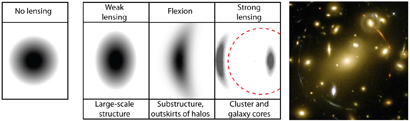
\includegraphics[scale=1.00]{img/WL_abel.jpg}
% 	\caption{(Left) Illustrations of the effect of a lensing mass on a circularly symmetric image. Weak lensing elliptically distorts the image, flexion provides an arc-ness and strong lensing creates large arcs and multiple images. (Right) Galaxy cluster Abell 2218, strongly lensed arcs can be seen in around the cluster. Every background galaxy is weakly lensed. From NASA, ESA, and Johan Richard (Caltech, USA).}
% 	\label{fig_WL_Abell}
% \end{figure}
\subsection{Large-scale structure}
Studying the large-scale structures (LSS) of the Universe is of a great importance for the cosmology. Since the clustering of matter on scales from galaxies to superclusters came from quantum fluctuations in the very early Universe with important modification by radiation and baryons, the LSS encode critical information about the contents of the Universe, the origin of the fluctuations, and the cosmic expansion background in which the structures evolved.

Measurements of large-scale power spectrum for the spatial distribution of matter as a function of redshift constrain the cosmic expansion history, the cosmological distance scale, the growth rate of structures, the mass of the neutrinos and the abundance of dark matter. This includes BAO measurement of the distance-redshift relation (as a standard ruler). The BAO with the growth of the LSS in the Universe form two robust probes of dark energy, and a potential discriminator between dark energy and modified gravity models. Beyond the dark energy, the large scale power spectrum is a probe of both neutrino mass and primordial non-gaussianity.

Long-term task of the LSS working group within DESC is \textit{Scalable optimal LSS analysis software development}.
\subsection{Galaxy clusters}
The observed number density and clustering of galaxy clusters as a function of mass and redshift provides a powerful toolset to constraining cosmology.  Galaxy clusters provided the first line of evidence for the existence of dark matter \cite{zwicky} and cluster mass-to-light ratio measurements suggested that the matter density in the universe was sub-critical \cite{Gott}. Galaxy clusters measurements are sensitive to both the expansion history and the growth of structure in the Universe enabling to distinguish between dark energy and modified gravity models for cosmic acceleration. Additional probes are measurements of the baryonic mass fraction in clusters, and of the tomographic lensing signatures through clusters.

The basic idea of cluster abundance studies is to compare the predicted space density of massive halos to the observed space density of clusters. The basic observables are the richness, the number of galaxies in a specified luminosity and color range. Halo abundance is sensitive to the amplitude of the matter power-spectrum $\sigma_8$\footnote{$\sigma_8$ is a linear fluctuation in the mass distribution on scales of $8h\mins$ Mpc} and the matter density $\Omega_m$, more precisely a combination of a form $\sigma_8\Omega_m^q$, with $q\approx0.4$ \cite{white}. The degeneracy between $\sigma_8$ and $\Omega_m$ can be broken by measuring abundances at a variety of masses.

Long-term task of the Cl working group within DESC is \textit{Optimizing magnification-based cluster mass calibration}.
\subsection{Strong lensing}
Strong gravitational lensing (SL) refers to the multiple imaging of a background object due to a massive foreground object (typically clusters of galaxies) -- see \autoref{fig_WL_Abell}. The resulting angular displacement, morphological distortion, and time delay can be used to measure dark energy parameters. Strong gravitational lensing time delays measure a combination of distances that combining with other dark energy probes can further constraint cosmological parameters. The time delays is also expected to test gravity on scales where the screening mechanisms is becoming active (more about screening mechanisms of modified gravities in \autoref{screen}).

Another independent way to measure dark energy parameters with SL is the analysis of systems with multiple sets of multiple images \cite{SL_in_CLGs}. The positions of these multiple images depend strongly on the detailed properties of the lens mass distribution and on the angular diameter distance ratios between the lens, source and observer, they encapsulate information about the underlying cosmology. This dependence on the geometry can be used to derive constraints on the cosmological parameters.

Long-term task of the SN working group within DESC is \textit{Explore multiple source plane cosmography as a competitive DE probe}.
\subsection{Redshift-space distortions}
%(and thus an apparent distance)
When we observe distant galaxies, two features determine their redshifts -- the Hubble expansion and their peculiar velocities. The peculiar velocities of galaxies thus cause them to appear displaced along the line of sight in redshift space. These displacements lead to redshift distortions in the pattern of clustering of galaxies in redshift space and make large scale galaxy clustering anisotropic. Redshift-space distortions (RSD) have the tremendous advantage of bearing information about the dynamics of galaxies. The strength of the anisotropy is governed by distortion parameter $\beta = f(z)/b(z)$, where $f(z)$ is the logarithmic growth rate of fluctuations. By modeling the full redshift-space galaxy power spectrum one can obtain combination of the product of the matter clustering amplitude and the growth rate.

Anisotropy of galaxy clustering offers an alternative to weak lensing and cluster abundances as a tool for measuring the growth of structures. RSD directly measure the rate at which structure is growing at the redshift of observation unlike WL and galaxy cluster measurements  which measure the rate of growth at multiple redshifts. RSD measurements can improve constraints on dark energy models and they can be used to constrain departures from GR by testing consistency of the growth and expansion histories. The key challenge in modeling RSD is accounting for nonlinear effects, including nonlinear or scale-dependent bias between galaxies and matter, at the level of accuracy demanded by the LSST`s precision.
\chapter{Dark Energy and~Modified Gravity}
\label{chpt:de_mg}
% In~this chapter, we describe one particular model of~modified gravity in~more detail -- the~$f(R)$ theory and~chameleon gravity. We will study the~behavior of~the~chameleon field in~spherical systems using numerical techniques. We also briefly introduce the~cosmological constant problem.
% Some review parts of this chapter has already been studied and described in author`s work \textcite{mastersthesis_vrastil}. In this work, we deal with the~same topic of the $f(R)$ gravity. We also use various notations and equations we already defined in~the~former work and we need them here, such as the~chameleon field $\chi$ and related equations. As we further develop the original study of the chameleon, we also took over some parts of the text (written in italics). We use the text in sections \hyperref[sec:fR]{\fR\ gravity}, \hyperref[sec_cham]{Chameleon Gravity}, and \hyperref[sec:other]{Other theories}, where a general overview of~other~interesting theories is presented. In section \hyperref[sec_cham]{Chameleon Gravity} we also extended our previous analysis of chameleon field on cosmological scales and we also extended the study of the chameleon in spherical systems on the scales of galaxy clusters.

% %%%%%%%%%%%%%%%%%%%%%%%
% % Standard LCDM model
% %%%%%%%%%%%%%%%%%%%%%%%
\section{Standard \LCDM\ model -- successes and issues}
Standard cosmological model, the \LCDM\ model or the concordance model, assumes that the Universe was created in the Big Bang from infinitely hot and dense energy and now is the Universe composed of about 5\% ordinary matter, 27\% dark matter, and 68\% dark energy \parencite{redefineLCDM}. The \LCDM\ model is based upon two theoretical models -- the Standard Model of Particle Physics and  the General Theory of Relativity. The model also assumes that the universe is homogeneous and isotropic on sufficiently large (cosmic) scales. The model is mathematically described above in \autoref{chpt:cosmo_evol}.

The \LCDM\ model represents general relativity with a cosmological constant \(\Lambda\) which is associated with dark energy and a universe containing sufficiently massive dark matter particles, i.e., cold dark matter. However, the nature of both dark energy and dark matter is unknown.

In 1948, \textcite{PhysRev.74.505.2} suggested that the elements could have been made during the early hot matter-energy phase associated with the Big Bang and predicted their representation -- hydrogen about 75\%, helium about 25\% and small amounts of deuterium, lithium, and other light elements.

The other great success of the Big bang model is prediction of the Cosmic Microwave Background (CMB) radiation and its temperature. In 1948, \textcite{1948Natur.162..774A} calculated the present temperature of the CMB to be about 5 K, remarkably close to the modern value of about 2.73 K, determined by the COBE satellite. In addition, the COBE results showed an extremely isotropic and homogeneous CMB. This led to the need for an inflationary phase \parencite{1981PhRvD..23..347G} of strongly accelerated expansion prior to the decoupling of photons from ordinary matter.

The \LCDM\ model has an additional major assumption about existence of dark matter. The notion of dark matter arose from observations of large astronomical objects such as galaxies and clusters of galaxies, which displayed gravitational effects that could not be accounted for by the visible matter. In particular, the observations of \textcite{1980ApJ...238..471R}, who measured the rotation curves for the luminous matter of many spiral galaxies together with the observations of \textcite{1978PhDT.......195B}, who compiled 21 cm rotation curves for neutral hydrogen gas that extended far beyond the luminous matter of each galaxy, showed that the composite rotation curves were essentially flat out to the edge of the 21 cm data. This implied that considerably more mass was required to be present in each galaxy. This invisible matter was called dark matter and since to date no dark matter has been definitely detected and the nature of dark matter remains unknown.

The notion of dark energy arose from two sets of observations of supernovae of Type Ia by \textcite{riess} and \textcite{1999ApJ...517..565P} that suggested that the expansion of the universe is accelerating. The conclusion from these observations was that the universe had to contain enough energy to overcome gravity. This energy was named “dark energy.”

\subsection{Cosmological constant problem}
\label{ssec:lambda}
Standard cosmological \LCDM\ model described above is in a good agreement with all measurements of CMB \parencite{planck_cosm}, type Ia supernovae \parencite{Abbott_2019}, or BAO \parencite{BAO_results}. However, this concordance model, and namely the cosmological constant, has some significant fundamental problems. Usually, the fine-tuning of the cosmological constant is presented as the main issue but the real issue with the cosmological constant is radiative instability, and the need to \textbf{repeatedly} fine tune whenever the higher loop corrections are included. We will describe here only the main idea behind these problems, for more detailed overview see e.g. \textcite{2015arXiv150205296P,2012CRPhy..13..566M}.

The action of the general relativity, together with the action describing matter, is
\eq{
	\label{eq:S_GR}
	S=\frac{\Mpl^2}{2}\int\dd^4x\dg\left(R-2\Lambda_B\right)+S_m[\psi_m;g_\uv]\,,
}
where $\Mpl\equiv(\sqrt{8\pi G})^{-1}$ is the reduced Planck mass, $R$ is the Ricci scalar (curvature), $\Lambda_B$ the bare cosmological constant and $S_m[\psi_m;g_\uv]$ represents the action of matter fields. The first term $(R)$ is the standard Einstein-Hilbert action. The \textit{bare} cosmological constant appears in the second term of the above expression and it is merely a new parameter of the total action. As it is compatible with general covariance this term appears to be totally natural from the relativistic point of view. The third term in the above equation denotes the generic matter action. Variation of the total action with respect to the metric tensor leads to the Einstein equations of motion
\eq{
    R_\uv-\frac12Rg_\uv+\Lambda_Bg_\uv=\frac{1}{\Mpl^2}T_\uv\,,
}
where the stress-energy tensor is defined by
\eq{
    T_\uv=-\frac{2}{\dg}\frac{\delta S_m}{\delta g^\uv}\,.
}
As shown by \textcite{1968SPhD...12.1040S}, when one takes into an account quantum field theory the picture is changed. The stress energy tensor of a field placed in the vacuum state is given by
\eq{
    \left\langle0\left|T_\uv\right|0\right\rangle=-\rho\vac g_\uv\,,
}
where $\rho\vac$ is the constant energy density of the vacuum. The vacuum fluctuations are just a specific type of energy and, in general relativity, all forms of energy gravitate. Therefore, the Einstein equations when quantum field theory is taken into account are
\eq{
    R_\uv-\frac12Rg_\uv+\Lambda\eff g_\uv=\frac{1}{\Mpl^2}T_\uv\,,
}
where
\eq{
    \Lambda\eff=\Lambda_B+\frac{1}{\Mpl^2}\rho\vac\,.
}
Therefore, we conclude that the effective cosmological constant is the sum of the bare cosmological constant and of a contribution originating from the vacuum fluctuations. The effective cosmological constant $\Lambda\eff$ is the quantity that one can observe and constrain when tests of the Einstein equations are carried out. The problem is that $\rho\vac$ is made of several terms which are all huge in comparison with the observed value of $\Lambda\eff$ and need to be fine-tunned.
\subsubsection{Phase Transitions}
\begin{sloppypar}
Another problem with fine-tuning of the cosmological constant comes from changes in the vacuum energy during phase transitions such as was the electro-weak phase transition. The contribution to the vacuum energy coming from the minimum of a potential of some field, in this case the Higgs field, changes as the field takes its new position after the transition. One can calculate this contribution \parencite{2012CRPhy..13..566M} and for the the mass of the Higgs boson $m_H=125$ GeV arrives at
\end{sloppypar}
\eq{
    \rho\vac^{EW}\simeq -10^{55}\rho\crit\,.
}
For the quantum chromo-dynamics transition, one can compute
\eq{
    \rho\vac^{EW}\simeq10^{45}\rho\crit\,.
}
If we fine-tune the vacuum energy to be zero today it had to be non-zero (and huge) before each of these transitions.
\subsubsection{Zero-Point Energy Density}
When we consider a simple real free scalar field with the potential $V(\Phi)=2m^2\Phi^2/2)$ we will arrive at the vacuum energy
\eq{
    \left\langle \rho \right\rangle = \left\langle0\left|T_{00}\right|0\right\rangle=\frac{1}{2\pi^3}\frac12\int\dd^3k\sqrt{k^2+m^2}\,.
}
This contribution to the cosmological constant blows up in the ultra-violet regime and is infinite. But this is nothing new in the quantum field theory. If we apply the dimensional regularization \parencite{tHooft:1972tcz} and subtract the pole as usual, one is left with finite energy density of the vacuum
\eq{
    \left\langle \rho \right\rangle = \frac{m^4}{64\pi^2}\ln{\left(\frac{m^2}{\mu^2}\right)}\,,
}
where $\mu$ is a regularization scale. We see that the contribution is proportional to the fourth power of the mass of the particle and therefore, e.g., the photon does not contribute to the vacuum energy density. The equation was derived for free scalar field but similar contributions with different pre-factors can be computed for all other fields. The overal vacuum energy density is then
\eq{
    \label{eq:vac_all}
    \rho\vac=\sum_in_i\frac{m_i^4}{64\pi^4}\ln{\left(\frac{m_i^2}{\mu^2}\right)} + \rho_B + \rho\vac^{EW} + \rho\vac^{QCD}\,,
}
where $n_H=1$ for the Higgs boson, $n_f=4$ for fermions and $n_V=3$ for massive vector fields. For the renormalization scale $\mu\simeq3\times10^{-25}$, as discussed in \textcite{2011arXiv1105.6296K}, one calculates the contribution from the zero-point energy of particles to be  $\rho\vac\simeq-2\times10^8$ GeV$^4$
\subsubsection{Radiative instability}
The one loop contributions \eqref{eq:vac_all} to the vacuum energy can be fine-tunned via the bare cosmological constant and associated $\rho_B$. Even though the cancellation has to be very precise (one part in $\sim10^{60}$) we can be fine with this solution. Problems come with two-loops correction which is not significantly suppressed with respect to the one loop contribution \todo{CITE}. Therefore, the cancellation imposed at one loop is completely spoilt, and one must retune the finite contributions in the counterterm to more or less the same degree of accuracy. If we go further, to the three loops, four loops, and so on, we are required to fine tune each time to an extreme accuracy. This is radiative instability and main cosmological constant problem.



% %%%%%%%%%%%%%%%%%%%%%%%
% % f(R)-gravity
% %%%%%%%%%%%%%%%%%%%%%%%
% \section{$f(R)$-gravity}
One of~the~simplest modified gravity models is the~so-called $f(R)$ gravity in~which we consider general functions of~the~Ricci scalar $R$ in~the~action
\eq{
	\label{eq:S_fr}
	S=\frac{\Mpl^2}{2}\int\dd^4x\dg\left[F(R)\right]+S_m[\psi_m;g_\uv]\,,
}
where $F(R)=R+f(R)$ and~$S_m$ is the~matter action with~matter fields $\psi_m$ which are minimally coupled to~gravity, i.e. they interact with~gravity only through the~determinant of~the~metric $\dg$ and~the~canonical kinetic term $-\frac12g^\uv\partial_\mu\psi\partial_\nu\psi$. The~matter fields $\psi_m$ obey standard conservation equations and~therefore the~metric $g_\uv$ corresponds to~the~Jordan frame.

Variation with~respect to~the~metric $g^\uv$ gives us the~equation of~motion
\eq{
	\label{eq:fR}
	F\R R_\uv-\frac{1}{2}F g_\uv+g_\uv\Box F\R-\nabla_\mu\nabla_\nu F\R=\frac{1}{\Mpl^2}T_\uv\,.
}
For~$f(R)=-2\Lambda$ the~standard Einstein gravity is reconstructed. Taking the~trace of~\eqref{eq:fR} we get
\eq{
	\label{eq:fR_tr}
	3\Box F\R+F\R R-2F=\frac{1}{\Mpl^2}T\,.
}
We see that there is a~propagating scalar degree of~freedom, so-called \textit{scalaron} $F\R$ with~mass $m^2=F\R/(3F\RR)$, which corresponds to~the~scalar field conformally coupled to~matter in~the~Einstein frame.

To~get the~inflation we need a~solution that approaches the~de Sitter solution characterized by vacuum space with~constant positive curvature. Thus $\Box F\R=0$ and~\eqref{eq:fR_tr} becomes
\eq{
	F\R R-2F=0.
}
For~example, the~model $F(R)=\alpha R^2$ gives rise to~an~asymptotically exact de Sitter solution and~can be responsible for~the~inflation in~the~early Universe. In~the~model $f(R) = R + \alpha R^2$, the~inflation ends when the~quadratic term becomes smaller than the~linear term. As at~the~present epoch is the~curvature very small this model is not suitable to~realize the~present cosmic acceleration. Models like $f(R)=-\alpha/R^n$ with~$\alpha>0,\ n>0$ could in~principle give rise to~the~present acceleration. However, these models do not satisfy local gravity constraints because of~the~instability associated with~negative values of~$f\RR$. Moreover, the~standard matter epoch is not present because of~a~large coupling between the~Ricci scalar and~the~non-relativistic matter.

There are four conditions for~the~viability of~\fR\ models \parencite{Amendola_2007}
\begin{itemize}
	\item $F\R>0\ (\rm{for\ } R>R_0)$, where $R_0$ is the~Ricci scalar at~the~present epoch,\\
	-- required to~avoid anti-gravity \parencite{2010deto.book.....A}\\
	\item $F\RR>0\ (\rm{for\ } R>R_0)$,\\
	-- required for~consistency with~local gravity tests \parencite{2005gr.qc.....5136O}, for~the~presence of~the~matter-dominated epoch \parencite{2007PhRvL..98m1302A} and~the~stability of~cosmological perturbations \parencite{2007PhRvD..75d4004S}\\
	\item $F(R)\rightarrow R-2\Lambda\ (\rm{for\ } R\gg R_0)$,\\
	-- required for~consistency with~local gravity tests \parencite{2008PhRvD..77b3507T} and~for~the~presence of~the~matter-dominated epoch \parencite{Amendola_2007}\\
	\item $0<\frac{RF\RR}{F\R}<1\ (\rm{for\ } F\R R-2F=0)$.\\
	-- required for~the~stability of~the~late-time de Sitter solution \parencite{1988PhLB..202..198M}
\end{itemize}
Some examples of~\fR\ models that satisfy these conditions:
\eq{
	f(R)&=-\mu R_c(R/R_c)^p	&\mbox{for\ }&0<p<1;\ \mu,R_c>0\,,\\
	f(R)&=-\mu R_c\frac{(R/R_c)^{2n}}{(R/R_c)^{2n}+1} 	&\mbox{for\ }&n,\mu,R_c>0\,,\\
	f(R)&=-\mu R_c\left[1-(1+R^2/R^2_c)^{-n}\right] 	&\mbox{for\ }&n,\mu,R_c>0\,,\\
	f(R)&=-\mu R_c\tanh(R/R_c)	&\mbox{for\ }&\mu,R_c>0\,.
}
One of~the~main predictions of~\fR\ gravity is a~different structure formation history than in~\LCDM. For~the~large-scale structure formation on~subhorizon scales \mbox{$k\gg H$} in~quasi-static approximation one gets the~modified equation for~matter density perturbation \parencite{2011RSPTA.369.4947B}
\eq{
	\ddot{\delta}_m+2H\dot{\delta}_m-4\pi G\eff \rho_m\delta_m\approx0\,,
}
where the~effective gravitational constant is defined by
\eq{
	G\eff \equiv\frac{G}{1+f\R}\frac{4k^2+3a^2m^2}{3k^2+3a^2m^2}\,.
}
On~scales much larger than the~scalaron Compton wavelength $m\mins$, gravity is unmodified aside from the~overall reduction factor $f\R$. However, on~smaller scales the~gravitational coupling increases by the~factor $4/3$. As the~scalaron mass $m$ and~the~factor $f\R$ depend on~curvature (local density), the~chameleon mechanism discussed earlier can prevent the~detection of~this effect in~the~Solar System.

%%%%%%%%%%%%%%%%%%%%%%%%%%%%%%
% Jordan vs. Einstein Frame
%%%%%%%%%%%%%%%%%%%%%%%%%%%%%%
\subsection{Jordan vs. Einstein Frame}
The~action \eqref{eq:S_fr} is described in~the~so-called Jordan frame, where the~matter fields are minimally coupled to~the~metric and~follow geodesics. We can also describe the~action in~the~so-called Einstein frame, where ``standard'' gravity is restored. Using the~conformal transformations
\eq{
\label{eins_trans}
\begin{split}
\tilde{g}_\uv &\equiv F\R g_\uv \,, \\
\phi &\equiv\Mpl\sqrt\frac32\ln F\R \,, \\
A(\phi) &\equiv F\R^{-1/2}\,, \\
V(\phi) &\equiv\frac{\Mpl^2}{2} \frac{F\R R - F}{F\R^2}\,,
\end{split}
}
we can rewrite the~action \eqref{eq:S_fr}
\eq{
\label{eq:S_ein_fr}
S=\int\dd^4x\dgt\left[\frac{\Mpl^2}{2}\tilde{R} - \frac12(\partial\phi)^2-V(\phi)\right]+S_m[\psi_m;A^2(\phi)\tilde{g}_\uv],
}
where tildes denote quantities in~the~Einstein frame. This action looks like the~Einstein-Hilbert action with~minimally coupled scalar but now the~matter fields are also coupled with~the~scalar field via factor $A(\phi)$. %Also from the~second row of~\eqref{eins_trans} can be seen why is the~Brans-Dicke parameter restricted to~be $\omega>-3/2$.

There is a~difference between whether one takes action \eqref{eq:S_fr} or \eqref{eq:S_ein_fr} to~be the~fundamental action defining the~modified gravity. In~the~former one, there is only one coupling constant $\beta$, defined by $A(\phi)=\exp(\beta\phi/\Mpl)$, for~all matter fields. If one takes the~action in~the~Einstein frame to~be the~fundamental one the~matter action is replaced by $S_m[\psi_m;A^2(\phi)\tilde{g}_\uv]\rightarrow S_i[\psi_i;A_i^2(\phi)\tilde{g}_\uv]$ where one can define the~coupling strengths $\beta_i$ to~the~different matter components to~be different. This is very important for~tests of~modified gravity. For~instance, if there is minimal coupling to~the~baryonic matter, $\beta_b=0$, Solar System or astrophysical tests do not constraint coupling strength to~the~cold matter $\beta_c$ whereas the~cosmological observations do.

Note that the~coupling constant for~\fR\ is $\beta=\sqrt{1/6}$ but for~other more general theories this coupling can vary. Even for~\fR\ theories, one expects that loop corrections can change the~coupling strength. Also, other theories such as the~Jordan--Brans--Dicke theory, Kaluza--Klein theories, and~higher derivative theories of~gravity, can be formulated in~two different ways \parencite{Faraoni:1998qx}.

These two conformally related frames are physically equivalent, i.e. physical observations are frame independent, but the~frame dependence of~cosmological perturbations has led to~confusion in~the~past. There have been many debates about the~(in)equivalence of~these frames \parencite{Postma:2014vaa} and~whether which one is the~physical \parencite{Faraoni:1999hp}. Many contradictory arguments (sometimes incorrect) of~both sides result in~confusion and~ambiguous viewpoints.

It has been shown in~\textcite{Magnano:1993bd} that these two frames are \textit{mathematically} equivalent, i.e. every solution in~one frame implies an~existence of~a~solution in~the~other frame and~can be mapped into this frame. The~confusion about their physical equivalence comes from interpretations of~experiment results. For~example, \textit{ordinary} cosmology described by Einstein’s theory leads to~an~expanding universe solution. Coming to~the~Jordan frame we can interpret the~scale factor as a~scalar field which is coupled to~matter. In~this case, the~redshift of~spectral lines is no longer interpreted as an~effect due to~the~expansion of~the~Universe, but due to~growth of~coupling constants such that the~present transition energies are higher than those in~the~past. Hence the~Jordan frame physicist does not see an~expanding Universe, but growing coupling constants. Nevertheless, the~measured redshift of~spectral lines is the~same for~both frames.

Both frames have some issues with~fundamental principles. In~the~Jordan frame, the~weak energy condition can be violated and~hence states with~the~negative energy are possible. Moreover, there is no guarantee of~stability of~the~ground state. All \textit{classical} fields are believed to~satisfy the~energy condition but no so in~quantum theories. On~the~other hand in~the~Einstein frame, the~weak energy condition is satisfied but due to~the~non-universal coupling of~the~matter fields, the~equivalence principle is violated. However, this violation is only weak and~can pass the~Solar system tests.

%%%%%%%%%%%%%%%%%%%%%%%%%%%%%%
% Screening Mechanisms
%%%%%%%%%%%%%%%%%%%%%%%%%%%%%%
\subsection{Screening Mechanisms}
We know that general relativity with~the~cosmological constant and~assumptions about the~cold dark matter can describe our universe very well. That means that any modified cosmology must be able to~recover \LCDM\ cosmology to~high accuracy. This is not normally an~issue. However, since modifications of~GR typically involve an~extra scalar degree of~freedom there are interactions with~matter that are unavoidable -- no symmetry can prevent all couplings to~the~standard model. This coupling to~matter means that there should be a~fifth force. Because we do not see any fifth forces or modifications of~gravity in~the~laboratory or in~the~Solar System we need to~suppress these fifth forces -- we need some sort of~a~\textit{screening mechanism}.

The~nature of~the~screening mechanisms can be different. Let us start from \eqref{eq:S_ein_fr} with~the~generalized kinetic term $-\frac12 Z(\phi,\partial\phi,...)(\partial\phi)^2$. We can solve the~equations of~motion for~the~background in~a~minimum of~a~potential $V(\phi)$ and~write $\phi=\phi_0+\delta\phi$, where $\phi_0$ is a~background solution and~$\delta\phi$ is a~fluctuation. The~Lagrangian density for~the~fluctuations to~the~second order (first order vanishes) is
\eq{
\LL\propto-\frac12 Z(\phi_0)(\partial\delta\phi)^2+\frac12 m^2(\phi_0)\delta\phi^2+\frac{\beta(\phi_0)}{M_p}\delta\phi\delta T,
}
where $m^2(\phi)\equiv V_{,\phi\phi}(\phi)$. Now, any of~these three terms can serve as a~screening term:
\begin{itemize}
	\item  \textit{Large inertia} -- a~large $Z$ makes it hard for~the~scalar to~propagate and~leads to~the~kinetic type of~the~screening, where first or second derivatives being important; e.g. Galileons \parencite{2009PhRvD..79f4036N}, massive gravity \parencite{2012RvMP...84..671H} or Vainshtein mechanism \parencite{2013CQGra..30r4001B};
	\item \textit{Large mass} --  a~large $m$ means the~scalar propagates only over short distances and~leads to~the~chameleon type of~the~screening, where in~regions of~high-density, such as on~the~Earth, the~field acquires a~large mass -- the~Chameleon mechanism \parencite{Waterhouse:2006wv};
	\item \textit{Weak coupling} -- a~small $\beta$ in~regions of~high density makes the~interaction with~matter fields weaker and~leads to~symmetron \parencite{2010PhRvL.104w1301H}) or varying dilaton \parencite{Damour:1994zq,2011PhRvD..83j4026B} theories.
\end{itemize}

% %%%%%%%%%%%%%%%%%%%%%%%%%%%%
% % {Chameleon Gravity
% %%%%%%%%%%%%%%%%%%%%%%%%%%%%
\section[Chameleon Gravity]{Hu-Sawicki \texorpdfstring{\textit{\lowercase{f}(R)}}{fR} Model and Chameleon Gravity}
\label{sec_cham}
One of~the~simplest modified gravity models is the~so-called $f(R)$ gravity in~which we consider general functions of~the~Ricci scalar $R$ in~the~action. We wish to~study a~class of~$f(R)$ models that accelerate cosmic expansion at~late times, without the~cosmological constant, while satisfying both cosmological and~Solar System tests. We consider the~family of~Hu-Sawicki $f(R)$ models \parencite{Hu-Saw}. The~action of~these models in~the~Jordan frame is given by 
\eq{
	\label{eq:S_fr}
	S=\frac{\Mpl^2}{2}\int\dd^4x\dg\left[R+f(R)\right]+S_m[\psi_m;g_\uv]\,,
}
where~$f(R)$ has a~broken power-law form
\eq{
	f(R)=-M^2\frac{c_1(R/M^2)^m}{c_2(R/M^2)^m+1}\,,
}
where the~mass scale $M^2\equiv\bar\rho_0/3\Mpl^2$, $m>0$, and~$c_1$ and~$c_2$ are dimensionless parameters such that at~high redshifts \LCDM\ cosmology is restored. This \fR\ gravity exhibits the~so-called chameleon mechanism. This mechanism uses the~large mass of~the~chameleon field in~high-density regions and~chameleon gravity can satisfy tests of~the~equivalence principle in~the~Solar System.

In~the~Jordan frame the~matter fields are minimally coupled to~the~metric and~follow geodesics. We can also describe the~action in~the~Einstein frame, where ``standard'' gravity is restored. Using the~conformal transformations of the metric, we can rewrite the~action \eqref{eq:S_fr} as
\eq{
\label{eq:S_ein_fr}
S=\int\dd^4x\dgt\left[\frac{\Mpl^2}{2}\tilde{R} - \frac12(\partial\chi)^2-V(\chi)\right]+S_m[\psi_m;A^2(\chi)\tilde{g}_\uv],
}
where tildes denote quantities in~the~Einstein frame. This action looks like the~Einstein-Hilbert action with~minimally coupled scalar but now the~matter fields are also coupled with~the~scalar field via factor $A(\chi)$. Varying the~action with~respect to~the~field $\chi$ one can obtain the~equation of~motion
\eq{
	\label{eom:cham}
	\Box\chi=V_{,\chi}-\sum_i\frac{\beta_i}{\Mpl}e^{4\beta_i\chi/\Mpl}g^\uv_{(i)}T^{(i)}_\uv,
}
where $T^{(i)}_\uv$ is the~stress-energy tensor for~the~$i$-th matter component.% For~a~perfect isotropic fluid the~equation of~motion is
% \eq{
% 	\Box\chi=V_{,\chi}+\sum_i(1-3w_i)\frac{\beta_i}{\Mpl}\rho_i e^{(1-3w_i)\beta_i\chi/\Mpl}.
% }
% This equation could be read as
% \eq{
% 	\Box\chi=V_{\eff,\chi}\left(\chi\right),
% }
% where the~effective potential $V_{\eff}$ is defined by
% \eq{
% 	V_{\eff}\left(\chi\right)\equiv V(\chi)+\sum_i\rho_i e^{(1-3w_i)\beta_i\chi/\Mpl}.
% }
% The~action of~a~chameleon scalar field $\chi$ in~the~Einstein frame is given by the~action \eqref{eq:S_ein_fr}. Varying the~action with~respect to~the~field $\chi$ one can obtain the~equation of~motion
% \eq{
% 	\label{eom:cham}
% 	\Box\chi=V_{,\chi}-\sum_i\frac{\beta_i}{\Mpl}e^{4\beta_i\chi/\Mpl}g^\uv_{(i)}T^{(i)}_\uv,
% }
% where $T^{(i)}_\uv$ is the~stress-energy tensor for~the~$i$-th matter component. For~a~perfect isotropic fluid the~equation of~motion is
% \eq{
% 	\Box\chi=V_{,\chi}+\sum_i(1-3w_i)\frac{\beta_i}{\Mpl}\rho_i e^{(1-3w_i)\beta_i\chi/\Mpl}.
% }
% This equation could be read as
% \eq{
% 	\Box\chi=V_{\eff,\chi}\left(\chi\right),
% }
% where the~effective potential $V_{\eff}$ is defined by
% \eq{
% 	V_{\eff}\left(\chi\right)\equiv V(\chi)+\sum_i\rho_i e^{(1-3w_i)\beta_i\chi/\Mpl}.
% }
% {\itshape
% If the~couplings $\beta_i$ are the~same for~each matter component with~the~same $w$ (we can omit the~radiation in~the~sum) and~the~overall density is $\rho=\sum_i\rho_i$, then the~effective potential reads
% \eq{
% 	V_{\eff}\left(\chi\right)\equiv V(\chi)+\rho e^{(1-3w)\beta\chi/\Mpl}.
% }
% For~the~quasi-static and~weak $(\beta\chi/\Mpl\ll1)$ field in~a~weak gravity background (the~Minkowski background) with~the~non-relativistic matter, the~equation further simplifies as
% \eq{
% 	\label{eq:cham}
% 	\Delta \chi=\frac{\beta}{\Mpl}\rho+V_{,\chi},
% }
% which looks like the~normal Poisson equation but with~an~extra non-linear term.
% }
% \subsection{Chameleon Force}
% {\itshape
% The~interaction of~the~chameleon field with~matter is described by the~conformal coupling \eqref{eins_trans}. Free matter fields $\psi_m^{(i)}$ follow geodesics of~the~Jordan frame metric. In~the~Einstein frame, they follow modified trajectories affected by the~chameleon field \parencite{Waterhouse:2006wv}
% \eq{
% \frac{\dd^2x^\mu}{\dd\tau^2}+\Gamma^\mu_{\alpha\beta}\dddd{x^\alpha}{\tau}\dddd{x^\beta}{\tau}=-\frac{\beta_i}{\Mpl}\left(2\chi_{,\alpha}\dddd{x^\alpha}{\tau}\dddd{x^\mu}{\tau}+g^{\beta\mu}\chi_{,\beta}\right).
% }
% Note that the~chameleon force violates the~weak Equivalence Principle only if there exist two matter species with~differing values of~$\beta_i$. In~the~non-relativistic limit, a~test particle of~mass $m$ of~species $i$ in~a~static chameleon field $\chi$ is moving under a~force $\mb{F}_\chi$ given by
% \eq{
% \label{cham_force}
% \frac{\mb{F}_\chi}{m}=-\frac{\beta_i}{\Mpl}\mb{\nabla}\chi
% }
% }
% \subsection{Chameleon mechanism}
% {\itshape
% As discussed previously, we need some sort of~a~screening mechanism to~avoid Solar System tests of~GR. It means as seen from \eqref{cham_force} that the~chameleon potential needs to~approach some constant value in~dense regions or at~least have a~marginally suppressed amplitude.

% Suppose we have a~background solution $\chi_0$ which minimizes the~effective potential with~$\rho=\rho_0$. For~small fluctuations $\chi=\chi_0+\delta\chi$ and~$\rho=\rho_0+\delta\rho$ we can linearize \eqref{eq:cham} to~obtain
% \eq{
% \label{eq:cham_lin}
% \Delta \delta\chi=\frac{\beta}{\Mpl}\delta\rho+m^2_0\delta\chi,
% }
% where
% \eq{
% m^2_0\equiv V_{,\chi\chi}(\chi_0).
% }
% Except for~the~screening term, the~equation \eqref{eq:cham_lin} has the~same behavior as the~Poisson equation for~the~Newtonian potential $\Phi_G$. For~a~spherically symmetric density profile, this gives solution
% \eq{
% \chi=\chi_0+2\beta\Mpl\Phi_G\left(r\right)e^{-m_0 r}.
% }
% As the~objects in~the~background become more massive (larger and/or denser) the~Newtonian potential grows larger (in~magnitude) and~so the~deviation of~$\chi$ from background solution $\chi_0$. At~some point, this deviation is no longer small and~the~potential term in~\eqref{eq:cham} cannot be treated perturbatively. It starts canceling the~first source term and~eventually the~field $\chi$ posses a~new value which minimizes the~effective potential inside an~object.

% This is the~essence of~the~chameleon mechanism. Let us derive the~mechanism more properly and~exactly.
% } %% itshape
% \subsection{Chameleon Profile}
% {\itshape
% \label{cham_prof}
% To~obtain the~chameleon behavior described above we need to~choose a~chameleon potential $V(\chi)$ with~the~right properties. To~have a~screening mechanism in~\eqref{eq:cham} we need $V_{,\chi}<0$ to~cancel the~source term and~$V_{,\chi\chi}>0$ to~have a~real mass of~the~field and~stable behavior of~perturbations.

% We wish to~find a~solution for~spherically symmetric matter distributions of~a~single species of~pressureless matter such that
% \begin{equation*}
% \rho(r)=
% \begin{cases}
% \rho_c & r<R_s \\
% \rho_0 & r>R_s,
% \end{cases}
% \end{equation*}
% where $\rho_c>\rho_0$. Further, we define $\chi_c$ and~$\chi_0$ with~their masses $m_c$ and~$m_0$ (the~masses of~small fluctuations about $\chi_c$ and~$\chi_0$) such as
% \begin{align*}
% V_{\eff,\chi}\left(\chi_c\right)_{|\rho=\rho_c}&\equiv0	&	m^2_c&\equiv V_{\eff,\chi\chi}\left(\chi_c\right) \\
% V_{\eff,\chi}\left(\chi_0\right)_{|\rho=\rho_0}&\equiv0	&	m^2_0&\equiv V_{\eff,\chi\chi}\left(\chi_0\right).
% \end{align*}
% In~the~background with~low density, the~curvature of~the~potential is much shallower, corresponding to~a~light scalar that mediates a~long-range force. Inside the~object of~high density, the~scalar acquires a~large mass, and~the~force shuts off.

% In~spherical coordinates assuming spherical symmetry, equation \eqref{eq:cham} becomes
% \eq{
% \label{eq_cham_r}
% \frac{\dd^2\chi}{\dd r^2}+\frac{2}{r}\dddd{\chi}{r}=\frac{1}{r}\frac{\dd^2\left(r\chi\right)}{\dd r^2}=V_{,\chi}\left(\chi(r)\right)+\frac{\beta}{\Mpl}\rho(r).
% }
% We must impose two boundary conditions which are
% \begin{align*}
% \dddd{\chi}{r}(r=0)&=0 \\
% \chi(r\rightarrow\infty)&=\chi_0.
% \end{align*}
% The~first one corresponds to~a~non-singularity of~the~solution at~the~origin while the~later one ensures that the~chameleon force vanishes at~the~infinity (as $\dd\chi/\dd r\rightarrow0$).

% The~equation \eqref{eq_cham_r} drives the~field $\chi$ toward the~$\chi_0$ outside the~object and~toward $\chi_c$ inside the~object. To~solve \eqref{eq_cham_r}, we must do several approximations. Outside the~object, we assume that the~field sits near the~extreme $\chi_0$ and~we can linearize our equation
% \eq{
% \frac{1}{r}\frac{\dd^2\left(r\chi\right)}{\dd r^2}=m^2_0(\chi-\chi_0),
% }
% with~the~decaying solution
% \eq{
% \chi(r)=-\frac{\beta}{4\pi\Mpl}\frac{\tilde{M}}{r}e^{-m_0 r}+\chi_0.
% }
% Note that the~integration constant $\tilde{M}$ is not generally the~mass of~the~object $M_c$ as in~the~case of~the~Newtonian potential because it is determined by the~field inside the~object which has different behavior than the~Newtonian potential. As we will see later, for~small Newtonian potentials (in~magnitude) this effective mass $\tilde{M}\approx M_c$ but as the~potential grows larger part of~the~object's mass is screened away $\tilde{M}< M_c$.

% Inside the~object, we use one of~the~two approximations based on~the~initial value of~$\chi_i\equiv\chi(0)$ -- either $\chi_i\approx\chi_c$ or $\chi_i\gg\chi_c$ .
% \subsubsection{Thin-shell regime}
% In~the~\textit{thin-shell} regime, the~field initially sits very close the~minimum $\chi_c$, i.e. we require
% \eq{
% (\chi_i-\chi_c)/\chi_c\ll1.
% }
% The~field is frozen near this value until the~friction term is sufficiently small to~allow the~field to~roll. This ``moment'' is denoted by $R_{roll}$. As soon as $\chi$ is displaced significantly from $\chi_c$ we may neglect the~potential term in~\eqref{eq_cham_r}. This gives us the~solution
% \eq{
% \chi(r)=
% \begin{cases}
% \chi_c & 0<r<R_{roll} \\
% \frac{\beta}{6\Mpl}\rho_cr^2+\frac{A}{r}+D & R_{roll}<r<R_s.
% \end{cases}
% }
% We have boundary conditions coming from the~requirement on~matching $\chi$ and $\dd\chi/\dd r$ at~$R_{roll}$, namely: $\chi=\chi_c$ and~$\dd\chi/\dd r=0$ at~$r=r_{roll}$. This fixes our constants and~the~solution is
% \eq{
% \label{eq_thin}
% \chi(r)=
% \begin{cases}
% \chi_c & 0<r<R_{roll} \\
% \frac{\beta\rho_c}{3\Mpl}\left(\frac{r^2}{2}+\frac{R^3_{roll}}{r}\right)-\frac{\beta\rho_cR^2_{roll}}{2\Mpl}+\chi_c & R_{roll}<r<R_s.
% \end{cases}
% }
% The~approximation of~separating the~solution into the~two regions only makes sense if $(R_s-R_{roll})/R_s\ll1$. Otherwise, there is no clear separation between the~two regions, and~one needs a~solution valid over the~entire range $0<r<R_s$. In~\autoref{sec:num_cham} we solve equation \eqref{eq_cham_r} numerically and~we will check these approximations against numerical solutions.

% With~approximation $(R_s-R_{roll})/R_s\ll1$, we can determine the~effective mass of~the~object $\tilde{M}$ from the~requirement $\chi(R_s^-)=\chi(R_s^+)$ and~$\dd\chi/\dd r(R_s^-)=\dd\chi/\dd r(R_s^+)$.
% \eq{
% \tilde{M}=\frac{3\Delta R_s}{R_s}M_c,
% }
% where
% \eq{
% \frac{\Delta R_s}{R_s}\equiv\frac{\chi_0-\chi_c}{6\beta\Mpl|\Phi_G(R_s)|}\approx\frac{R_s-R_{roll}}{R_s}\ll1.
% }
% This qualitative derivation of~the~thin-shell regime is using too much assumptions and~can be done more precisely without ignoring some of~the~terms but then it is harder to~see the~principle of~the~thin-shell effect. For~more details see e.g. \textcite{Tamaki:2008mf,2007PhRvD..75f3501M,Waterhouse:2006wv}.
% \subsubsection{Thick-shell regime}
% In~the~\textit{thick-shell} regime, the~field is initially sufficiently displaced from the~minimum -- $\chi_i\gg\chi_c$ that it begins to~roll almost immediately (no friction term). Hence the~interior solution is most easily obtained by taking the~$R_{roll}=0$ in~\eqref{eq_thin} and~replacing $\chi_c$ by $\chi_i$
% \eq{
% \label{eq_thick}
% \chi(r)=\frac{\beta\rho_cr^2}{6\Mpl}+\chi_i\ \ \ 0<r<R_s.
% }
% By matching the~interior and~exterior solutions, we obtain
% \eq{
% \begin{split}
% \chi_i &=\chi_0-3\beta\Mpl\Phi_G(R_s)\\
% \tilde{M} &=M_c,
% \end{split}
% }
% which is the~linear regime with~no screening. From the~definition of~$\Delta R_s/R_s$ we also obtain
% \eq{
% \frac{\Delta R_s}{R_s}\equiv\frac{\chi_0-\chi_c}{6\beta\Mpl|\Phi_G(R_s)|}>1.
% }
% \subsubsection{Thin-shell suppression factor}
% The~chameleon force outside the~object (where experiments take place) comparing to~the~Newtonian force is
% \eq{
% \begin{split}
% \label{eq_cham_suppression}
% \frac{F_{thick}}{F_N}&=2\beta^2 \\
% \frac{F_{thin}}{F_N}&=2\beta^2\frac{3\Mpl\left(\chi_0-\chi_c\right)}{\beta\rho_cR^2_c},
% \end{split}
% }
% where we ignore the~term $m_0 r\ll1$. Therefore for~the~coupling $\beta$ of~order unity, the~chameleon force is as strong as gravity unless it is screened away by the~thin-shell effect.
% } %% itshape
%%%%%%%%%%%%%%%%%%%%%%%%%%%%%%
% HU-SAWICKI
%%%%%%%%%%%%%%%%%%%%%%%%%%%%%%
% \subsection{Hu-Sawicki \texorpdfstring{\textit{\lowercase{f}(R)}}{fR} Model}
The~Hu-Sawicki models correspond to~chameleon gravity with~the~potential
\eq{
	V(\chi) &= \Mpl^2\Lambda-\frac{\beta\bar\rho_0}{n\Mpl}\left(2\beta\Mpl\Phiscrz\right)^{1-n}\chi^n\,, \\
    V_{,\chi}(\chi) &= -\frac{\beta}{\Mpl}\bar\rho_0\left(\frac{2\beta\Mpl\Phiscrz}{\chi}\right)^{1-n}\,,
}
where $\beta=\sqrt{1/6}$ and~the~power-law exponent $n$ and~screening potential $\Phiscrz$ are now the~free parameters of~the~theory.% The~screening potential has the~following relation to~the~present scalaron value in~$f(R)$-gravity:
% \eq{
%     \Phiscrz=\frac{3}{2}\ln{(1+f_{R0})}\approx\frac{3}{2}f_{R0}.
% }
The~chameleon obeys the~equation of~motion \eqref{eom:cham} which reduces for~our study case (non-relativistic pressureless matter) to
\eq{
\label{eq:cham_husa}
	\Delta \chi = \frac{\beta}{\Mpl}\rho - \frac{\beta}{\Mpl}\bar\rho_0\left(\frac{2\beta\Mpl\Phiscrz}{\chi}\right)^{1-n}
}
% We rescale the~equations to~units in~which we can clearly see the~role of~the~screening potential $\Phiscr$ and~its relation to~the~gravitational potential $\Phi_G$. We start by defining a~few special values of~the~chameleon potential -- the~current background value
% \eq{
% 	\chi_0\equiv2\beta\Mpl\Phiscrz\,,
% }
% the~background value at~a~given time (for~a~matter-dominated universe)
% \eq{
% 	\chi_a(a)\equiv \chi_0 a^{3/(1-n)}
% }
% and~the~value of~the~screening potential at~a~given time
% \eq{
% 	\Phiscra\equiv\Phiscrz a^{\frac{5-2n}{1-n}}\,.
% }
% With~these definitions, we rewrite equation \eqref{eq:cham} as
% \eq{
% \label{eq:cham_u}
% 	\Delta\left(\chi/\chi_a\right)= C_\chi(a)\left[1+\delta-\left(\frac{\chi_a}{\chi}\right)^{1-n}\right]\,,
% }
% where the~pre-factor $C_\chi(a)$ is defined by
% \eq{
% 	C_\chi(a)\equiv\frac{3H_0^2\Omega_m}{2\Phiscrz}a^{-3\frac{2-n}{1-n}}=\left(a\mu\Phiscra\right)^{-1}\,.
% }
% \subsubsection{Linear prediction}
% Equation \eqref{eq:cham_u} is similar to~the~Poisson equation for~the~gravitational potential and~gives meaning to~the~screening potential $\Phiscra$. If we assume $\chi\approx\chi_a$, then
% \eq{
% 	\label{eq:chi__scr_mean}
% 	\Delta\left(\chi/\chi_a\right) \approx \left(\mu\Phiscra\right)^{-1}\frac{\delta}{a} = \Delta\left(\Phi_G/\Phiscra\right)
% }
% and~we can write down a~linear solution as
% \eq{
% \label{eq:chi_lin_x}
% 	\chi(\mb x, a) = \chi_a(a)\left(1 + \frac{\Phi_G(\mb x, a)}{\Phiscra(a)} \right)\,.
% }
% Here we can clearly see the~role of~the~(time-dependent) screening potential $\Phiscra$ -- as long as $|\Phi_G| < \Phiscra$ we have a~valid solution but once the~gravitational potential is large enough (in~its negative values) the~linear solution breaks down, as the~chameleon field would become negative.

% We may derive a~more accurate solution in~Fourier space. If the~chameleon field sits near its background value, i.e. $\chi=\chi_a\left(1 + \delta\tilde\chi \right)$, where $\delta\tilde\chi \ll 1$, we can rewrite \eqref{eq:cham_u} as
% \eq{
% 	\Delta\delta\tilde\chi=\frac{m^2}{1-n}\delta + m^2\delta\tilde\chi\,,
% }
% where the~mass of~the~chameleon field is
% \eq{
%     \label{eq:chi_m}
% 	m^2(a)\equiv\frac{1-n}{a\mu\Phiscra}\,.
% }
% This equation has a~solution in~$k-$space of~the~form
% \eq
% {
% \label{eq:chi_lin_k}
% 	\hat{\chi}(k)=-\frac{\chi_a}{1-n}\frac{m^2}{m^2+k^2}\hat{\delta}(k) = -\frac{\beta\bar\rho}{\Mpl}\frac{\hat{\delta}(k)}{k^2+m^2}\,.
% }

% The~other regime, which can be solved approximately, is the~screened regime inside massive objects. When the~solution \eqref{eq:chi_lin_x} breaks down, and~if $\delta(x)$ is approximately constant, the~solution of~equation \eqref{eq:cham_u} is
% \eq{
% 	\chi=\frac{\chi_a}{\left(1+\delta\right)^{1/(1-n)}}\,.
% 	\label{eq:chi_bulk}
% }
% Because $\chi_a$ is constant in~space the~chameleon force \eqref{cham_force} vanishes in~this screened regime.

% In~\autoref{fig:chi_evol} we show the~evolution of~background parameters of~the~chameleon field -- Compton wavelength $\lambda_c=m^{-1}$, background value of~the~chameleon field $\chi_a$ and~the~screening potential $\Phiscra$ -- for~different values of~the~power-law exponent $n$ and~the~screening potential $\Phiscrz$.

% \begin{figure}[hbt]
% \centering
% 	\begin{subfigure}{1.0\textwidth}
%         \includegraphicscustomlegend{simulations_approx/chi/chi_evol}
% 	\end{subfigure}
% 	\begin{subfigure}{1.0\textwidth}
% 		\includegraphicscustom{simulations_approx/chi/chi_evol}
% 	\end{subfigure}
%     \caption{Evolution of~background parameters of~the~chameleon field. From top to~bottom: Compton wavelength $\lambda_c$, chameleon field $\chi_a$ and~screening potential $\Phiscra$.}
%     \label{fig:chi_evol}
% \end{figure}

% The~background value of~the~Compton wavelength informs us about the~global behavior of~the~chameleon field whereas the~screening potential describes its behavior locally. At~high redshifts, the~chameleon's Compton wavelength is too short to~have any effects -- on~large scales, due to~its low background value, and~on~small scales due to~a~low value of~the~screening potential. At~lower redshifts, the~chameleon field starts to~affect matter, initially only on~small scales but with~the~passage of~time also on~large scales. We thus expect the~strongest effects to~be on~small scales.
\subsection{Numerical solutions}
\label{sec:num_cham}
In~this section, we will show the~results of~numerical solutions of~the~chameleon profile. We will solve the~equations for~the~Hu-Sawicki \fR\ model, \eqref{eq:cham_husa}. In~this section we will focus only on~systems with~spherical symmetry, i.e. we will solve the~following equation
\eq{
	\label{eq:cham_husa_r}
	\frac{\dd^2\chi}{\dd r^2}+\frac{2}{r}\dddd{\chi}{r} = \frac{\beta}{\Mpl}\rho - \frac{\beta}{\Mpl}\bar\rho_0\left(\frac{\chi_0}{\chi}\right)^{1-n}
}
Our algorithm for~finding solutions to~\eqref{eq:cham_husa_r} uses the~shooting method \parencite{10.5555/42249} and~is based on~the~original algorithm of~\textcite{mastersthesis_vrastil}. We further improved the~code applicability, readability, and~its parametrization. The~code is publicly available at~\code{\url{https://github.com/vrastil/chi_r_solver}}. We will denote $\Req$ the~\textit{equivalence radius} -- radius at~which the~Newtonian potential equals the~screening potential $|\Phi_G(\Req)|=\Phi_s$. By letting the~equivalence radius posses also negative values such as $(1+|\Req|/R_s)|\Phi_G(0)|=\Phi_s$ we can clearly distinguish between the~linear $(\Req<0)$ and~the~screening $(\Req>0)$ regime.

% \subsubsection{Stars}
% {\itshape
% We will first consider a~case where some approximate solutions exist -- a~compact spherical object of~constant density $\rho_c$ surrounded by the~background of~density $\rho_0$ as discuss in~\autoref{cham_prof}. We expect that for~low-mass objects the~chameleon field will track the~Newtonian potential while for~massive objects the~chameleon field will be frozen inside the~sphere and~outside it will be following the~Newtonian behavior but with~decreased amplitude.
% }

% In~\autoref{fig:starlike} we show results for~the~chameleon profile. We used the~notation $\tilde\chi\equiv(\chi-\chi_0)/2\beta\Mpl$ for~better comparison with~the~Newtonian potential. We see that for~$\Phiscr>\Phi_G$ we have an~unscreened solution as expected. For~lower values of~$\Phiscr$ the~field is frozen inside the~object and~have lower amplitude outside the~object as expected from analytical solutions.
% \begin{figure}
% 	\centering
% 	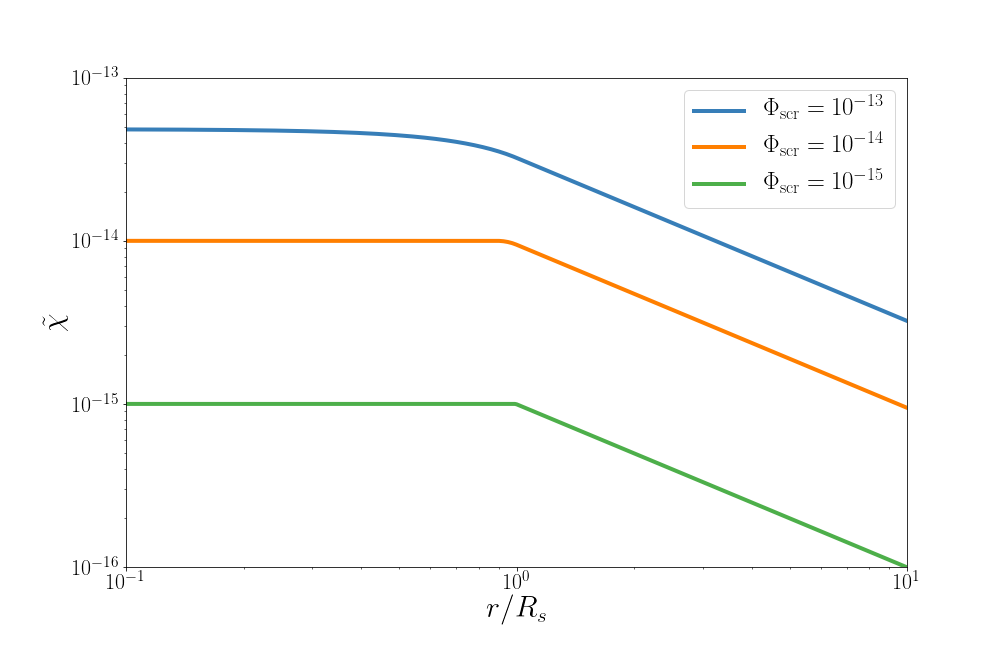
\includegraphics[width=1.0\linewidth]{{spherical_cham/starlike}.png}
% 	\caption{Chameleon profile for~several screening potentials. The~top solution is in~the~linear regime and~is identical to~the~gravitational potential. The~other two solutions are in~the~screened regime and~the~amplitude of~the~field is suppressed.}
% 	\label{fig:starlike}
% \end{figure}

% {\itshape
% Let us focus on~the~regime which cannot be treated analytical, i.e. regime between thin-shell and~thick-shell solutions. This regime corresponds to~the~situation when the~linear approximation (thick-shell) breaks down inside the~object, i.e. the~gravitational potential cancels screening potential somewhere inside the~object. We will denote $\Req$ the~\textit{equivalence radius} -- radius at~which the~Newtonian potential equals the~screening potential $|\Phi_G(\Req)|=\Phi_s$. By letting the~equivalence radius posses also negative values such as $(1+|\Req|/R_s)|\Phi_G(0)|=\Phi_s$ we can clearly distinguish between the~linear $(\Req<0)$ and~the~screening $(\Req>0)$ regime.}

% In~\autoref{fig:starlike_forces} we show the~behavior of~the~chameleon fifth force in~this regime. We see that for~the~linear regime the~fifth force is as strong as standard gravity (up to~the~factor $2\beta^2$). For~$\Req\ll R_s$ the~chameleon field manages to~catch up with~the~linear solution inside the~object and~there is no screening outside. As the~$\Req$ grows the~field is not able to~catch up with~the~linear solution while inside the~object and~the~force outside is screened.
% \begin{figure}
% 	\centering
% 	
\includegraphics[width=1.0\linewidth]{{spherical_cham/starlike_forces}.png}
% 	\caption{Chameleon force relative to~the~standard gravitational force for~several screening potentials (given through the~equivalence radius). For~$\Req\ll R_S$ there is no screening outside the~object. As the~$\Req$ grows the~chameleon enters the~screened regime.}
% 	\label{fig:starlike_forces}
% \end{figure}

\subsubsection{NFW Halo}
The~Navarro-Frenk-White (NFW) profile proposed by \textcite{1996ApJ...462..563N} describes the~distribution of~cold dark matter. The~NFW profile of~matter overdensity is given by
\eq{
	\label{NFW_rho}
	\delta\rho_{\rm NFW}(r)=\frac{\rho_c}{r/r_s\left(1+r/r_s\right)^2},
}
where $\rho_c$ is the~density scale and~$r_s$ is the~scale radius. We will also be using the~dimensionless radius $x\equiv r/r_s$. The~total mass of~the~halo is divergent (logarithmically) so we take a~cut-off at~the~radius $r_{200}$, which is defined as the~radius at~which the~density is 200 times the~critical density. Then the~mass of~the~halo is
\eq{
	M_{200}=\int_0^{r_{200}}4\pi r^2\rho(r)\dd r=4\pi\rho_cr_s^3\left(\ln(1+c)-\frac{c}{c+1}\right),
}
where $c\equiv r_{200}/r_s$ is the~concentration of~the~halo. For~a~given mass the~halo is fully characterized by the~concentration.

% For~NFW halo the~density is not constant as in~the~case of~compact spherical objects (stars). The~chameleon mass and~the~screened solution are therefore also not constant and~one does not have analytical solutions as in~the~case of~stars. However, for~realistic halo, the~density varies on~scales much larger than the~Compton wavelength of~the~chameleon. In~such cases, we can treat the~field as frozen in~the~same sense as in~the~case of~stars. Therefore we expect the~chameleon field to~behave in~a~similar way as in~the~case of~stars, i.e. to~follow the~Newtonian potential in~the~linear case and~to~have screened behavior for~more massive halos.

In~\autoref{fig:nfwlike_forces} we show the~chameleon fifth force. We see that the~behavior is indeed similar to~stars although the~field catches up much later. This is because there is no sudden drop in~density (and~mass of~the~field) where the~chameleon can start to~behave as free but rather the~mass is slowly dropping. This indicates that it will be much harder to~detect the~chameleon fifth force on~scales of~galaxies than for~star-like objects. This is of~course true only assuming the~screening potential is the~same on~all scales.
\begin{figure}
	\centering
	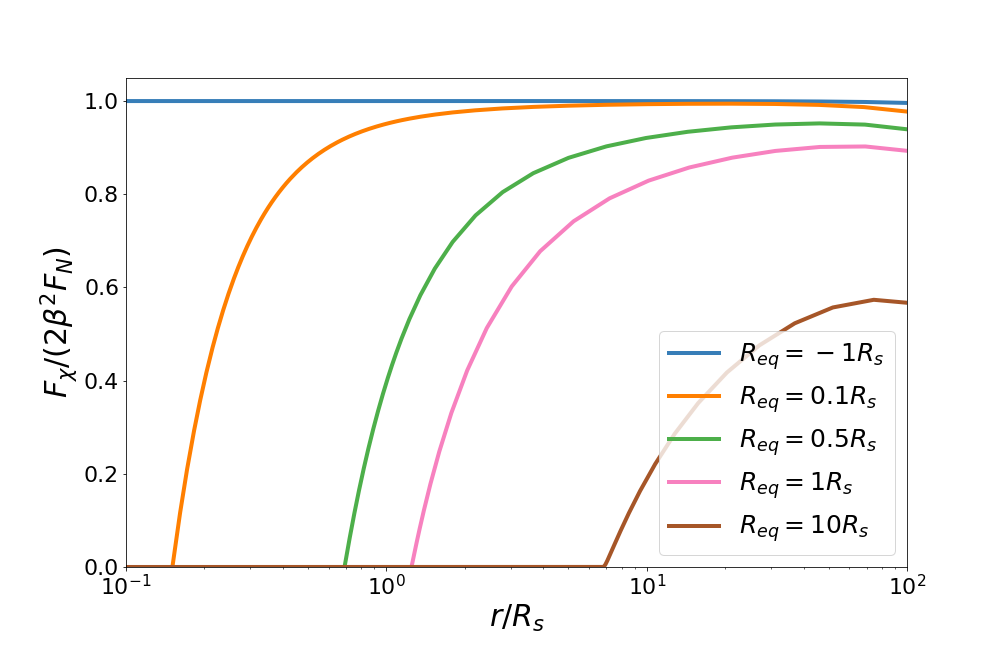
\includegraphics[width=1.0\linewidth]{{spherical_cham/nfwlike_forces}.png}
	\caption{Chameleon force relative to~the~standard gravitational force for~several screening potentials (given through the~equivalence radius). For~$\Req\ll R_S$ there is no screening outside the~object. As the~$\Req$ grows the~chameleon enters the~screened regime.}
	\label{fig:nfwlike_forces}
\end{figure}

The~meaning of~the~screening potential and~its connection to~the~Newtonian potential in~\eqref{eq:chi__scr_mean} is given by the~value of~the~field at~the~background, i.e. value that minimizes right side of~\eqref{eq:cham_u}. However, objects like stars or galaxy halos do not sit directly in~the~overall average density of~the~universe but rather in~galaxy halo or halo of~the~cluster of~galaxies. Therefore the~value of~the~effective screening potential is given by the~density of~the~background object we can consider as being in~infinity relative to~the~scale of~the~studied object. In~\autoref{fig:nfwlike_pot_eff} we show the~value of~this effective screening potential for~a~cluster of~galaxies of~a~typical size -- $M=10^{14} M_\odot, c=4$. We see that the~screening potential is greatly reduced in~inner parts of~the~galaxy cluster halo. For~this reason, we do not think it much likely to~observe the~effects of~the~chameleon field on~scales smaller than Mpc.

\begin{figure*}
	\centering
		\begin{subfigure}{1.0\linewidth}
			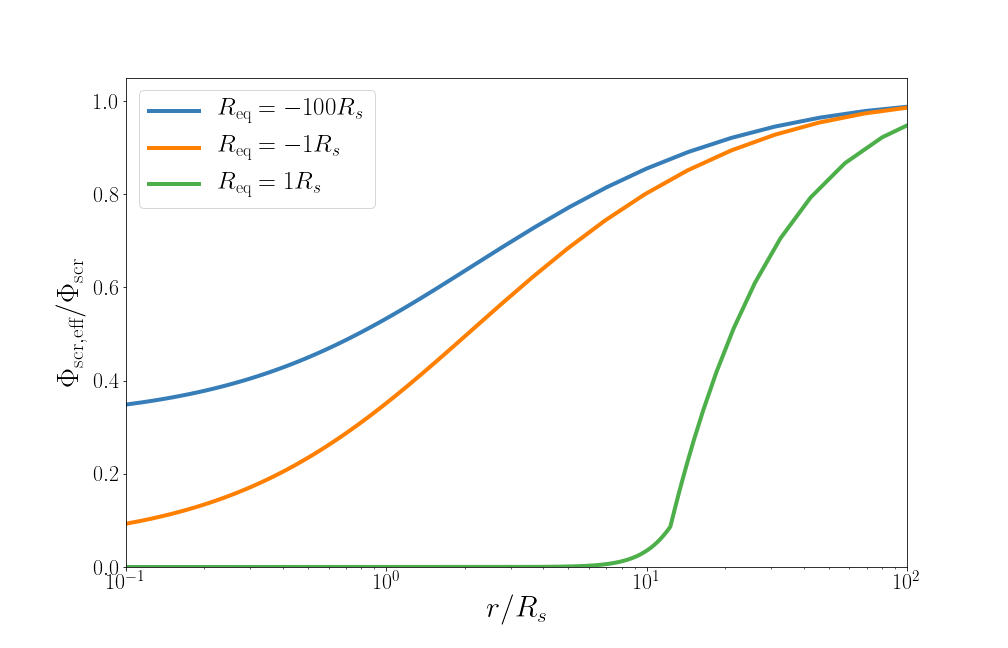
\includegraphics[width=1.0\linewidth]{{spherical_cham/nfwlike_pot_eff}.png}
		\end{subfigure}
		\begin{subfigure}{1.0\linewidth}
			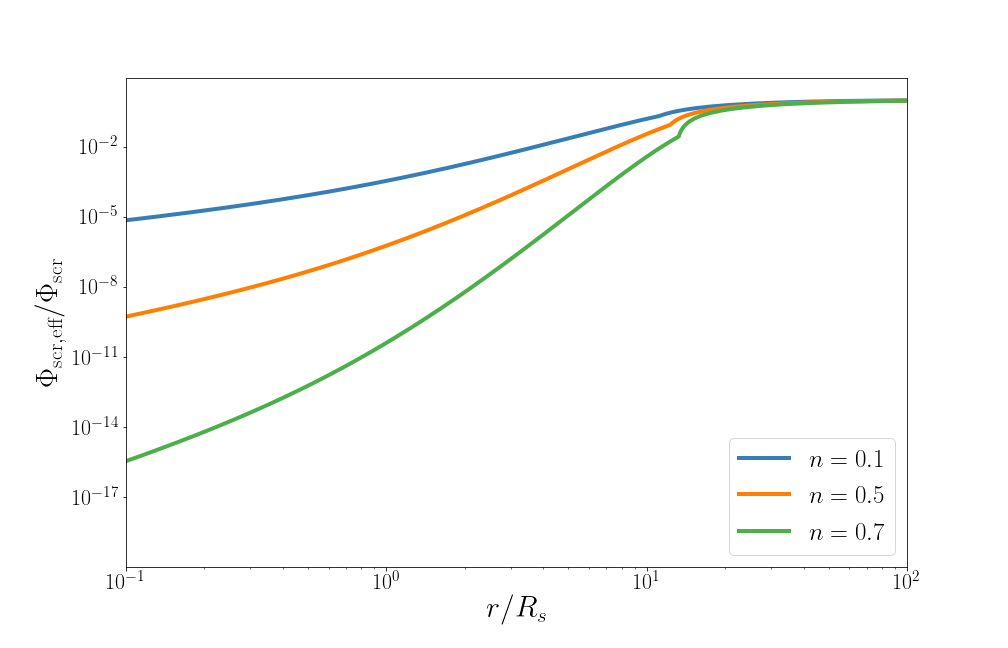
\includegraphics[width=1.0\linewidth]{{spherical_cham/nfwlike_pot_eff_n}.png}
		\end{subfigure}
		\caption{Effective screening potential relative to~the~screening potential for~a~cluster of~galaxies, $M=10^{14} M_\odot, c=4$. The~top Figure is shown for~several screening potentials (given through the~equivalence radius) while the~bottom for~different chameleon parameter $n$.}
		\label{fig:nfwlike_pot_eff}
\end{figure*}

As the~chameleon affects only non-relativistic matter it can be detected using a~combination of~dynamical measurements and~lensing measurements. Therefore, we considered what would be the~difference between the~mass distribution of~a~galaxy cluster measured via lensing (true mass) and~via dynamics of~enclosed galaxies. In~\autoref{fig:clustersYs} we plot this ratio for~five real clusters (simulated as having ideal NFW profile), see their parameters in~\autoref{tab:clusters}, and~for~four different values of~the~screening potential. We see that except for~the~case $\Phiscr=1$ one would need very precise (and~nowadays unrealistic) measurements of~the~mass distribution. We are therefore left with~only cosmological scales of~tens of~Mpc and~larger to~study the~chameleon. We will study this case in~\autoref{chpt:app_sims}.
\begin{table}[hbt]
	\centering
	\begin{tabular}{lcc|lcc}
		\hline \hline
		Cluster & $c$ & $M$ & Cluster & $c$ & $M$ \\
		\hline
		ClG 0054-27 & $1.2$ & $0.42\cdot10^{14}$ &
		Cl 0016+1609 & $2.1$ & $1.12\cdot10^{14}$ \\
		MS 2137.3-2353 & $13$ & $2.9\cdot10^{14}$ &
		ClG 2244-02 & $4.3$ & $4.5\cdot10^{14}$ \\
		MS 0451.6-0305 & $5.5$ & $18\cdot10^{14}$ & & & \\
		\hline \hline
	\end{tabular}
	\caption{Properties of~clusters simulated as perfect NFW halos: concentration $c$ and~mass $M [M_\odot]$. Parameters are taken from \textcite{2007MNRAS.379..190C}}
	\label{tab:clusters}
\end{table}

\begin{figure*}[!hbt]
\begin{adjustwidth}{-1cm}{-1cm}
	\centering
		\begin{subfigure}{0.5\linewidth}
			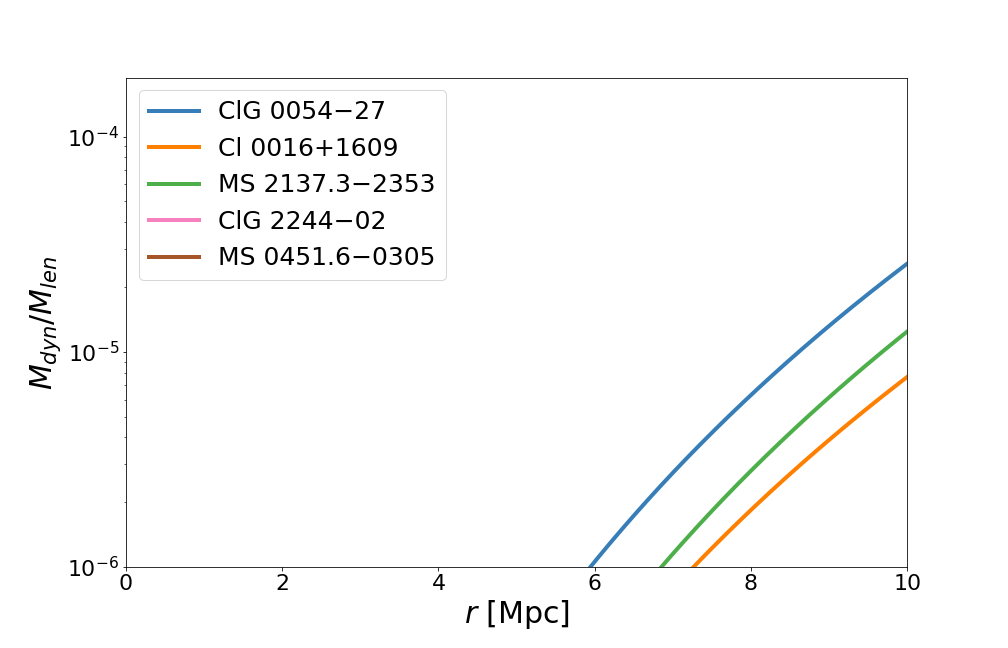
\includegraphics[width=1.0\linewidth]{{spherical_cham/clustersYs_-6}.png}
			\caption{$\Phiscr=10^{-6}$}
		\end{subfigure}%
		\begin{subfigure}{0.5\linewidth}
			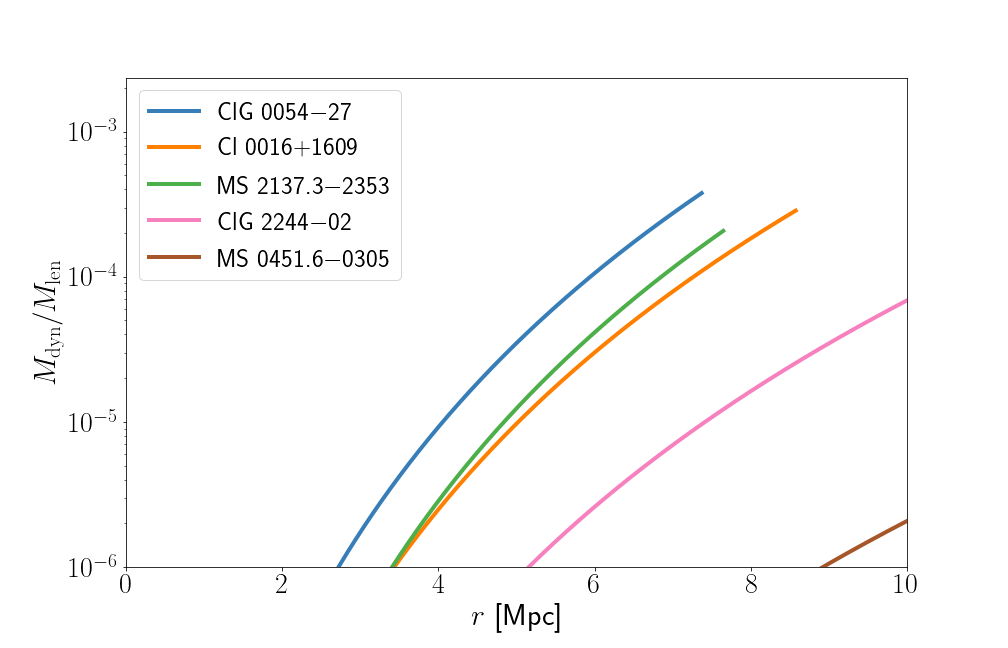
\includegraphics[width=1.0\linewidth]{{spherical_cham/clustersYs_-4}.png}
			\caption{$\Phiscr=10^{-4}$}
		\end{subfigure}
		\begin{subfigure}{0.5\linewidth}
			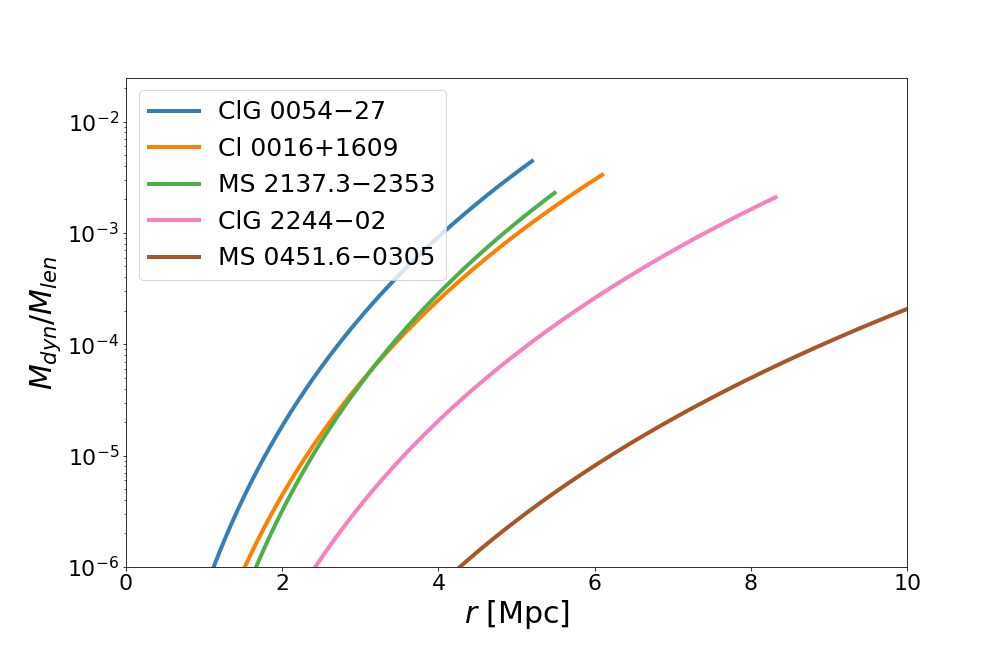
\includegraphics[width=1.0\linewidth]{{spherical_cham/clustersYs_-2}.png}
			\caption{$\Phiscr=10^{-2}$}
		\end{subfigure}%
		\begin{subfigure}{0.5\linewidth}
			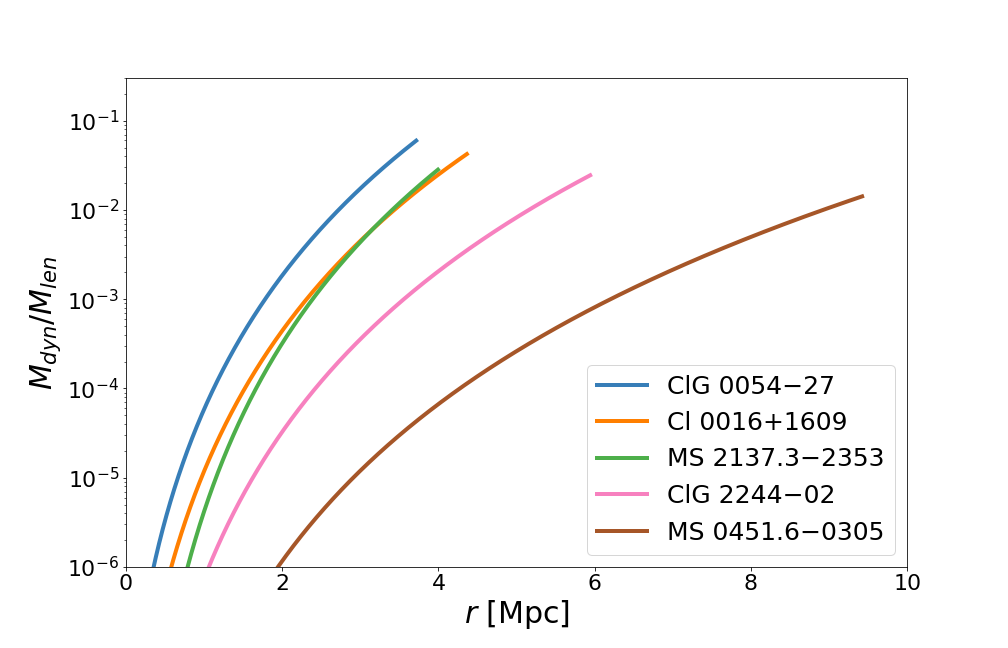
\includegraphics[width=1.0\linewidth]{{spherical_cham/clustersYs_0}.png}
			\caption{$\Phiscr=10^{0}$}
		\end{subfigure}
	\end{adjustwidth}
		\caption{Effective dynamical mass of~the~clusters relative to~the~actual (lensing) mass of~the~cluster. Cluster properties are shown in~\autoref{tab:clusters}.}
		\label{fig:clustersYs}
\end{figure*}

% %%%%%%%%%%%%%%%%%%%%%%%%%%%%
% % Other theories
% %%%%%%%%%%%%%%%%%%%%%%%%%%%%
% \section{Other theories}
In this section we briefly mention some of the other theories od modified gravity. This list is in no way complete and serves only as an example of different approaches to modifications of gravity. See references for further reading.
\subsection{Quintessence}
Quintessence, from the Latin ``fifth element'', is according to ancient and medieval philosophy the fifth element, or ether, supposed to be the constituent matter of the heavenly bodies after air, fire, earth, and water. The name quintessence, or the $Q$ component, was first used by \textcite{1998PhRvL..80.1582C} for the canonical scalar field $\phi$ evolving along a potential $V(\phi)$. Such a dynamical field can reproduce the late-time acceleration with the equation of state $w=w(t)\approx1$. Although quintessence can alleviate the coincidence problem of dark energy via the so-called tracker solution, it still suffers by the fine-tunning problem as the potential needs to be flat enough to lead to the slow-roll inflation today with an energy scale $\rho_{DE}\simeq10^{-120}\Mpl^4$ and a mass scale $m_\phi\lesssim10^{-33}$ eV. However, such fine-tuned potentials can be constructed within the framework of particle physics.

Quintessence is one of the simple models of dark energy as it is a canonical scalar field that interacts with all the other components only through standard gravity. The Lagrangian density for the quintessence field is
\eq{
\label{Qlagr}
\LL_\phi=-\frac12(\partial\phi)^2-V(\phi)
}
We can compute the stress-energy tensor as
\eq{
T^\phi_\uv\equiv\frac{-2}{\dg}\frac{\delta(\dg\LL_\phi)}{\delta g^\uv}=\partial_\mu\phi\partial_\nu\phi-g^\uv\left(\frac12(\partial\phi)^2+V(\phi)\right).
}
Now, the energy density and pressure are given by components of the stress-energy tensor. For FLRW background and $\phi$ only time-dependent we get
\eq{
\rho_\phi=-T^0_0=\frac{1}{2}\dot{\phi}^2+V(\phi)\ \ \ \ p_\phi=\frac{1}{3}T^i_i=\frac{1}{2}\dot{\phi}^2-V(\phi).
}
Equation of state for the quintessence is then
\eq{
\label{eosQ}
w\equiv\frac{p}{\rho}=\frac{\dot{\phi}^2-2V(\phi)}{\dot{\phi}^2+2V(\phi)}\,.
}
We require the condition $w<-1/3$ to realize the late-time cosmic acceleration, which translates into the condition  $\dot{\phi}^2<V(\phi)$, i.e. the potential needs to be shallow enough for the field to evolve slowly along the potential. For a slow-rolling field such as $\dot{\phi}\ll V(\phi)$ equation of state \eqref{eosQ} reduce to $w\approx-1$ as indicated by cosmological measurements.

The variation of \eqref{Qlagr} with respect to $\phi$ gives us the equation of motion for the scalar field $\phi$
\eq{
\ddot{\phi}+3H\dot{\phi}^2+V_{,\phi}=0\,.
}

Depending on which term and when determines the evolution of the field, the quintessence models have been dynamically classified into \textit{freezing} models and \textit{thawing} models \parencite{2005PhRvL..95n1301C}. In the freezing models the field was rolling along the potential in the past, but the movement gradually slows down as the field approaches the minimum of the potential $(\dot{\phi}\rightarrow0)$ and the system enters the phase of the cosmic acceleration $(w\rightarrow-1)$. In the thawing models, the field was initially frozen $(\dot{\phi}\approx0)$ in the early matter era because of the Hubble friction (the term $H\dot{\phi}$) until recently and then it begins to evolve once $H$ drops below $m_\phi$ and $w$ evolves from $-1$.

A potential of the freezing models is for example
\eq{
\label{Qtr}
V(\phi)=M^{4+n}\phi^{-n}\ (n>0),
}
which appears in the fermion condensate model as dynamical supersymmetry breaking \parencite{1999PhRvD..60f3502B}. This potential does not possess a minimum and hence the field rolls down the potential toward infinity. Another example of potential in the freezing models is
\eq{
V(\phi)=M^{4+n}\phi^{-n}\exp{(\alpha\phi^2/\Mpl^2)},
}
which can be constructed in the framework of supergravity \parencite{1999PhLB..468...40B}. This potential has a minimum at which the field is eventually trapped (corresponding to $\dot{\phi}=0$ and hence $w=-1$).

The broader class of potentials belonging to the thawing models are so-called hilltop quintessence models \parencite{2008PhRvD..78l3525D}, in which the scalar field is rolling near a local \textbf{maximum} in the potential but it begins to roll down around the present. A particular example that is well-described by this model is the pseudo-Nambu-Goldstone Boson (PNGB) model of \textcite{1995PhRvL..75.2077F}, for which the potential is given by
\eq{
V(\phi)=M^{4}\left[\cos{(\phi/f)}+1\right].
}
\subsection{K-essence}
Quintessence models are based on a scalar field with a canonical kinetic term and a slowly varying potential. However, in the context of particle physics there appear scalar fields with non-canonical kinetic terms. In \textcite{1999PhLB..458..209A} it is shown that a large class of scalar fields with non-canonical kinetic terms can, without the help of potential terms, drive an inflationary evolution starting from rather generic initial conditions. The Lagrangian density for the k-essence is
\eq{
\label{Klagr}
\LL_K=P(\phi, X),
}
where $X=-\frac12(\partial\phi)^2$ is the canonical kinetic energy and the function $P(\phi, X)$ must vanish for $X\rightarrow0$ (otherwise there would be some potential term). 

The energy-momentum tensor of the k-essence is given by
\eq{
T^K_\uv\equiv\frac{-2}{\dg}\frac{\delta(\dg\LL_K)}{\delta g^\uv}=P_{,X}\partial_\mu\phi\partial_\nu\phi+g^\uv P,
}
which is of the form of a perfect fluid, $T_\uv=(\rho+p)u_\mu u_\nu+g_\uv p$, with a four-velocity $u_\mu=\partial_\mu\phi/\sqrt{2X}$, pressure $p_K=P$ and energy density
\eq{
\rho_K=2XP_{,X}-P.
}
The equation of state of the k-essence is then
\eq{
w_K=\frac{p_K}{\rho_K}=\frac{P}{2XP_{,X}-P},
}
which is $w_K\approx-1$, as long as the condition $XP_{,X}\ll P$ is satisfied.

In the low-energy effective string theory appear higher-order derivative terms coming from $\alpha$ and loop corrections to the tree-level action \parencite{2003PhR...373....1G}. The k-essence action for these theories is for example
\eq{
P=K(\phi)X+L(\phi)X^2.
}
Phantom or ghost scalar fields with a negative kinetic energy $-X$ and $w\lesssim-1$ can also fit the current observations. These ghost fields generally suffer from a quantum instability problem unless higher-order terms in $X$ or $\phi$ are taken into account in the Lagrangian density \parencite{2010deto.book.....A}. The action of the so-called dilatonic ghost condensate model is \parencite{2004JCAP...07..004P}
\eq{
P=-X+e^{\kappa\lambda\phi}X^2/M^4.
}
\subsection{Gauss-Bonnet Dark Energy Models}
In \fR\ gravity one adds the general function of the Ricci scalar. But in principle, one can add general functions of the Ricci and Riemann tensors as well, e.g. $f(R,R_\uv R^\uv,R_{\alpha\beta\gamma\delta}R^{\alpha\beta\gamma\delta},...)$ \parencite{2005PhRvD..71f3513C}. These Lagrangians are generally plagued by the existence of ghosts.  However, there exists a combination of Ricci and Riemann tensors that keeps the equations at second-order in the metric and does not necessarily give rise to instabilities -- so-called Gauss-Bonnet term $\GB$ coupled to a scalar field
\eq{
\GB\equiv R^2-4R_\uv R^\uv+R_{\alpha\beta\gamma\delta}R^{\alpha\beta\gamma\delta}.
}
The Gauss-Bonnet term is the unique invariant for which the highest (second) derivative occurs linearly in the equations of motion and thus ensuring the uniqueness of solutions. The Gauss-Bonnet term naturally arises as a correction to the tree-level action of low-energy effective string theories \parencite{2000PhR...337..343L}. The starting action is given by
\eq{
S=\int\dd^4x\dg\left[\frac{\Mpl^2}{2}R-\frac{\gamma}{2}\left(\nabla\phi\right)^2-V(\phi)+f(\phi)\GB\right],
}
where $\gamma=\pm1$ (+1 for the canonical scalar). For more details see \textcite{2005PhRvD..71l3509N,2006JCAP...06..004N,2013PhRvD..87h4037C}.
\subsection{Braneworld Models}
In the braneworld model of Dvali, Gabadadze, and Porrati \parencite[DGP model][]{2000PhLB..485..208D} the 3-brane is embedded in a Minkowski bulk spacetime with infinitely large extra dimensions. The theory gives rise to the correct 4D potential at short distances whereas at large distances the potential is that of a 5D theory. The action of the theory is
\eq{
S=\frac{M^3_{(5)}}{2}\int\dd^5X\dgt\tR+\frac{\Mpl^2}{2}\int\dd^4x\dg R + \int\dd^4x\dg \LL_m,
}
where $g_{AB}(X)=g_{AB}(x,y)$ denotes a 5D metric for which the 5D Ricci scalar is $\tR$ and $M_{(5)}$ is the 5D Planck mass. Capital letters are used for 5D quantities $(A,B=0,1,2,3,5)$. The brane is located at $y=0$. The induces 4D metric on the brane is denoted by
\eq{
g_\uv(x)\equiv\tilde{g}_\uv(x,y=0).
}
The cross-over scale $r_0$ is defined by
\eq{
r_0\equiv\frac{\Mpl^2}{2M^3_{(5)}}.
}
At short distances $r\ll r_0$ gravity behaves as usual 4D theory, i.e the gravitational potential has correct $1/r$ behavior (except small logarithmic repulsion term). On the other hand at large distances $r\gg r_0$ the potential scales as $1/r^2$ according to the laws of 5D theory.

The presence of the extra dimension has severe consequences on the cosmology as well. It can be shown \parencite{2010deto.book.....A,2009PhLB..674..237M} that the matter-dominated Universe approaches the de Sitter solution $H=r_0\mins$. This cosmological solution drives our Universe into the self-inflationary regime without dark energy. From $H_0\approx r_0\mins$ we get $M_{(5)}\approx10-100$ MeV.
\subsection{Massive Gravity}
The idea to give a mass to the graviton (infrared modification of gravity) is not new and has been investigated since the first years of General Relativity. It is a less minimal theory than \fR\ theories or modified gravities with an extra scalar field because it introduces three new degrees of freedom rather than one. By giving a mass $m$ to the graviton we deform the classical potential to the Yukawa profile $\sim\frac1r e^{-mr}$ which departs from the classical one at distances $r>1/m$. By choosing the graviton mass to be of the order of the Hubble constant $m\sim H$ one can hope to explain the acceleration of the universe without dark energy.

The simplest theory for a non-self-interacting massive graviton is the Fierz-Pauli theory of \textcite{1939RSPSA.173..211F}. The action for a single massive spin 2 particle in flat space, carried by a symmetric tensor field $h_\uv$ is
\eq{
\begin{split}
S=&\int\dd^4x\Big[-\frac12\partial_\lambda h_\uv\partial^\lambda h^\uv+\partial_\mu h_{\nu\lambda}\partial^\nu h^{\mu\lambda}-\partial_\mu h^\uv\partial_\nu h \\
&+\frac12\partial_\lambda h \partial^\lambda h-\frac12 m^2\left(h_\uv h^\uv-h^2\right)\Big]+S_m.
\end{split}
}
Any other combination of $h_\uv h^\uv$ and $h^2$ would lead to instabilities. Varying the action with respect to $h_\uv$ yields the equation of motion
\eq{
R_\uv-\frac12Rg_\uv+\frac12m^2(h_\uv-h\eta_\uv)=\frac{1}{\Mpl^2}T_\uv,
}
where all quantities are linearized around $\eta_\uv$.

Because of the so-called vDVZ discontinuity (``van Dam-Veltman-Zakharov'') in the propagator of a graviton, the Fierz-Pauli theory leads to different physical predictions from those of GR regardless the mass of the graviton (even when $m\to0$). The Vainshtein mechanism \parencite{1972PhLB...39..393V} allows in principle to get rid of the vDVZ discontinuity by introducing non-linear Fierz-Pauli gravity.

The Vainshtein mechanism is another example of the screening mechanism and restores the continuity with GR on scales below the so-called Vainshtein radius $r_V$, defined as
\eq{
r_V\equiv(GM/m^4)^{1/5}.
}
Much below the Vainshtein radius, which grows as the graviton's mass approaches $0$, only linear terms play a crucial role and the GR is restored.

For more about the massive gravity and the Vainshtein mechanism see e.g. \textcite{2013CQGra..30r4001B,2012RvMP...84..671H}.

\subsection{Acceleration without Dark Energy}
So far we studied some kind of dark energy -- either in the form of an exotic matter or by modifying gravity itself. But this need for dark energy as an explanation of the acceleration comes from our observations which are based on the presumption of the homogeneous and isotropic Universe. What we observe are different expansion rates at different distances rather than an increase in the expansion rate at all distances. But this can be caused by strong inhomogeneities in the distribution of matter rather than by an accelerating Universe.
\subsubsection{Void models}
The basic idea behind void models is that we live in the middle of a huge spherical region which is expanding faster because it is emptier than the outside. That means that the Universe as a whole does not accelerate but that we observe an \textit{apparent} cosmic acceleration. The edge of this void should be located around $z\sim0.3-0.5$, the value at which in the standard interpretation we observe the beginning of the acceleration. These models are described by the Lema\^\i tre-Tolman-Bondi (LTB) spherically symmetric metric -- the generalization of a FLRW metric in which the expansion factor along the radial coordinate is different relative to the surface line element $\dd\Omega^2$ \parencite{2013JCAP...02..047D,2006PhRvD..73h3519A}.

The inhomogeneous LTB model matches to the supernovae data and the location of the first acoustic peak of the CMB temperature power spectrum but cannot satisfactorily reproduce the entire CMB angular power spectrum \parencite{2011JCAP...02..013C}. The observed isotropy of the CMB radiation implies that we must live close to the center of the void -- nearer than 15 Mpc \parencite{2006PhRvD..74j3520A}. Moreover, there is no valid mechanism at present to explain the formation of such huge inhomogeneities, let alone one with our Galaxy near the center.
\subsubsection{Backreaction}
Unlike the void models, which regard the acceleration as an apparent one, \textit{backreaction} models try to explain the cosmic acceleration by arranging inhomogeneities so that the deviation from the FLRW metric can produce a real acceleration \parencite{2011CQGra..28w5002S,2004JCAP...02..003R,2005PhRvD..72b3507M}. Because GR equations are non-linear, averaging the inhomogeneities and then solving the GR equations (which is the usual approach) is not the same as first solving the full (inhomogeneous) GR equations and then averaging them -- the expected value of a non-linear function is not the same as the non-linear function of the expected value.

Any large inhomogeneities must be concealed from our sight to fit observations. Strong peculiar velocities instead of strong density fluctuations can do this job, but there are strong constraints on peculiar velocities from e.g., the kinematic Sunyaev--Zel'dovich effect. Moreover, the accompanying anisotropy is another source of observable effects difficult to accommodate with current observations.

\section{Parametrization of models}
We saw in the previous chapter that at the background level the evolution is governed by Friedman equations \eqref{eq:Friedmann} -- \eqref{eq:Friedmann-continuity} and consequently omega parameters \eqref{eq:omega} and Hubble parameter $H$ which can be obtained, e.g., from distance measurements. As we discussed, the cosmological constant is not the only possible explanation of the accelerated expansion and the equation of state \(w\) of dark energy does not have to be exactly \(w=-1\). For the arbitrary equation of state $w_{DE}=p_{DE}/\rho_{DE}$ in the flat Universe with a negligible contribution of radiation we can obtain the following equation
\eq{
    \label{eq:w_de}
    w_{DE}(z)=\frac{(1+z)(E^2(z))'-3E^2(z)}
                   {3\left[E^2(z)-\Omega_{m,0}(1+z^3)\right]}\,,
}
where a prime denotes derivative with respect to \(z\). We see that \(w_{DE}\) cannot be determined solely from \(E(z)\) (obtainable through distance measurements) and we need also present density of matter \(\Omega_{m,0}\). However, if we parametrize \(w_{DE}\) in some way as it is usually done through measurements of \(E(z)\) at several redshifts we can constraint both \(w_{DE}\) and \(\Omega_{m,0}\).

Several parametrization  of \(w_{DE}\) have been proposed so far. We can write such parametrization  in the form
\eq{
    w_{DE}=\sum_{n=0}w_nx_n(z)\,,
}
where he expansions can be given by
\eq{
    & \rm{(i) Redshift:}      & x_n(z) &= z^n\,, \\
    & \rm{(ii) Scale factor:} & x_n(z) &= (1-a)^n=\left(\frac{z}{1+z}\right)\,, \\
    & \rm{(iii) Logarithmic:} & x_n(z) &= \left[\ln\left(1+z\right)\right]^n\,.
}
Parametrization (ii) is usually written for \(n\leq1\) as \(w=w_0+w_a(1-a)\).

For the generic \fR\ gravity, the equation of state is given by \parencite{2013qopu.conf...73B}
\eq{
    w_{DE} = \frac{-(1/2)(F\R R-F)+\ddot F\R+2H\dot F\R-(1-F\R)\left(2\dot H + 3H^2\right) }
                  {(1/2)(F\R - F) - 3H\dot F\R + 3 (1-F\R)H^2}\,,
}
which then can be compared with observations \eqref{eq:w_de}. For different examples of evolution of $w_{DE}$ see, e.g., \textcite{2020arXiv200707717A}.
\chapter{Cosmological Simulations}
\label{chpt:cosmo_sim}

%% full approximation scheme \parencite[FAS, see, e.g.,][]{MG_overview}

In this chapter we will use the following notation: box size $L$ [$\Mpch$], number of particles $\Np$, number of force mesh points $\Nf$, number of power-spectrum mesh points $\Na$, number of runs $N$, number of time-steps $\Nt$ and a derived parameter, the particle mass $m$ $[M_\odot]$. This notation is summarized in \autoref{tab:sim_param}.

\begin{table}
\begin{tabular}{ll}
    \hline \hline
    Symbol & Definition \\
    \hline
    $L$ & box size in units of $\Mpch$ \\
    $\Np$ & number of particles \\
    $\Nf$ & number of force mesh points \\
    $\Na$ & number of power-spectrum mesh points \\
    $N$ & number of runs \\
    $\Nt$ & number of time-steps \\
    $m$ & particle mass in units of $[M_\odot]$ \\
    \hline \hline
\end{tabular}
\caption{Summary of symbols used for simulation parameters.}
\label{tab:sim_param}
\end{table}


\section{\nbody\ problem}
Many problems in physics, including cosmology, involve particle systems with each particle interacting with all other particles present. In astronomy there is a gravitational interaction between starts, galaxies and cluster of galaxies, depending on scale which we are studying. The challenge of efficiently carrying out the related calculations is generally known as the \nbody\ problem.

The main problem is following -- we have $N_p$ particles all interacting gravitationally with each other. To compute a trajectory of even a single particle involves computing trajectories of all other particles as the gravitational force is dependent on time-varying positions of other particles. That means that at each time-step we have to compute force from all other $N_p$ particles and we need to compute these forces for each of $N_p$ particles. This leaves us with complexity of \(\OO(N_p^2)\). This brute force approach can be used only for small systems and is computationally unimaginable for large systems in cosmology which typically involve \(N_p\sim10^{9}\) particles.

This direct approach is generally referred to as the Particle-Particle (PP) method \parencite{Hockney:1988:CSU:62815}. Although computationally expensive the accuracy in the force calculation is of machine precision. To be able to simulate large systems of particles we need to drop the accuracy of continuous positions and use discrete positions for force calculations. In our code we use two main methods for force calculations -- the Particle-Mesh algorithm (PM) and grid-based methods, both of them we describe in more details below.
\subsection{Time integration}
The accurate time integration is a very important part of any \nbodysim. While there are many different methods to integrate particle trajectories \parencite[see e.g.][]{Hockney:1988:CSU:62815} we describe here one of the most used one in collisionless simulations -- the Leapfrog integrator.

The leapfrog integrator is an example of a symplectic integrator. Symplectic integrators exactly solve an approximate Hamiltonian. As a consequence, the numerical time evolution is a canonical map and preserves certain conserved quantities exactly, such as the total angular momentum, the phase-space volume, and the Jacobi constants. The idea is to approximate the Hamiltonian \(H\) governing motion of particles with an approximat one
\eq{
    \tilde H=H+H\err\,,
}
where \(H\err\) is the error Hamiltonian. Provided that \(\tilde H\) and \(H\) are time-invariant, the energy error is bounded at all times. The goal now is to find \(\tilde H\) that can be solved exactly by simple numerical means and minimises \(H\err\). Defining the combined phase-space coordinates \(w\equiv(x,p)\) the Hamilton’s equations are
\eq{
    \dot w=\HH w\,,
}
where \(\HH\equiv\{\cdot,H\}\) is an operator acting on \(w\) through Poisson bracket. Hamilton’s equations have then the formal solution
\eq{
    w(t+\Delta t)=e^{\Delta t\HH}w(t)\,.
}
\begin{sloppypar}
The operator \(e^{\Delta t\HH}\) can be split, in an approximate sense, into a succession of discrete but symplectic steps, each of which can be exactly integrated. The most common choice is to separate out the kinetic and potential energies, \({H=T(p)+V(x)}\), such that we can split
\end{sloppypar}
\eq{
    \label{eq:kdk}
    e^{\Delta t\HH}= e^{\Delta t(\TT+\VV)}\approx e^{\frac12\Delta t\VV}e^{\Delta t\TT}e^{\frac12\Delta t\VV}\,,
}
where operators \(\TT\equiv\{\cdot,T\}\) and \(\VV\equiv\{\cdot,V\}\) are known as drift and kick, as they only change either the positions (drift) or velocities (kick). Because these operators are non-commutative, the central relation in \eqref{eq:kdk} is only approximately true. This operator splitting is extremely useful, because the new equations have simple solution:
\eq{
    e^{\Delta t\TT}
    \begin{pmatrix}
        x \\
        p \\
    \end{pmatrix}=
    \begin{pmatrix}
        x+\Delta t\ p \\
        p \\
    \end{pmatrix}
    \mspace{20mu}\rm{and}\mspace{20mu}
    e^{\Delta t\VV}
    \begin{pmatrix}
        x \\
        p \\
    \end{pmatrix}=
    \begin{pmatrix}
        x \\
        p-\Delta t\ \nabla V \\
    \end{pmatrix}\,.
}
The splitting \eqref{eq:kdk}, also known as kick-drift-kick (KDK), is second order accurate, whereas simpler splitting only into one kick and one drift is first order accurate. The same accurcy and results has also similar splitting into drift-kick-drift which we use in our integrator.
\section{Particle-Mesh algorithm}
\label{sec:PM}
As we mentioned in the introduction in order to effectively compute forces on particles one has to abandon continuous position and solve the forces using discretized positions. The idea of the PM method is that we set up a mesh (grid) over the computational box, and then solve the gravitational potential (i.e. Poisson’s equation \eqref{eq:poisson_lin}) at the meshpoints. Forces at the meshpoints can then be obtained by calculating the gradient of the potential. The four principal steps of the particle-mesh calculation are:
\begin{enumerate}
    \item assign mass to the mesh,
    \label{it:pm_1}
    \item solve the field equation on the mesh,
    \label{it:pm_2}
    \item calculate the mesh-defined force field,
    \label{it:pm_3}
    \item interpolate to find forces on the particles,
    \label{it:pm_4}
\end{enumerate}
where the forces found at the last step are used to integrate the equations of motion.
\subsection{Assignment schemes}
In step \ref{it:pm_1} and \ref{it:pm_4} we make a connection between discrete mesh and continuous positions of the particles. In the first we need to distribute mass of all particles onto the mesh and in the last step, on the contrary, we need to interpolate forces known on the discrete mesh onto particles with continuous positions. There are several ways of assigning the particle masses to the discrete density function $\delta$ and discrete force $-\nabla\Phi$ to the particles:

\subsubsection{Nearest gridpoint (NGP)}
The mass of each particle $m_i$ is assigned as a whole to the gridpoint closest to the particle. Similary, force on particles is given by force on the nearest gridpoint. Although computationally the simplest, NGP as a zero-order interpolation offer lowest accuracy and the interparticle force changes discontinuously as particles cross cell boundaries.

\subsubsection{Cloud-in-Cell (CIC)}
The mass of each particle is weighted over the eight closest cells while the the weighting in each dimension is proportional to the distance between particle and the mesh. CIC scheme is more costly in terms of number of arithmetic operations per particle per timestep than NGP but offers better accuracy as first order (linear) interpolation. The CIC interpolation function in one dimension is
\eq{
    w(x-x_p)=
    \begin{cases}
        1-\frac{|x-x_p|}{H} & |x-x_p|<H\,\\
        0 & \rm{otherwise}
    \end{cases}
}
where $x$ is the position of a mesh point, $x_p$ position of the partice and $H$ the distance between mesh points. The three-dimensional interpolation function is \(W(\mathbf x)=w(x_1)w(x_2)w(x_3)\). The CIC scheme is somewhere in the middle between oversimplistic NGP and higher order interpolations which offer greater accuracy and smoother transitions but at the cost of much greater computational resources -- second order interpolation (triangular shaped cloud, TSC) involves 27 cells, third order 64, and etc. CIC gives a much smoother force than the NGP scheme (piecewise linear) and reduces the amplitude of fluctuations in the interparticle forces as the particles are displaced with respect to the mesh. In our code we use the CIC scheme.
\subsubsection{Mixed schemes}
The NGP and CIC schemes both employ mass assignment functions which are the same as their force interpolation functions. A result of this symmetry is that they conserve momentum, i.e., the forces between a pair of particles are equal and opposite, and the force of a particle upon itself (the self force) is zero. A possible variation is to use a mass assignment function which is different from the force interpolation function. In such cases, symmetry still causes the force between pairs of particles to be equal and opposite, but no longer ensures that the self force is zero. At best, the presence of the self force presents a nonphysical restriction on the timestep and, at worst, it is disastrous.

\subsection{Solution of the field equations}
An efficient method for the solution of the field equations is a necessary requirement for the practical implementation of the particle simulation algorithms that have been described. For linear Poisson’s equation \eqref{eq:poisson_lin} the most used method is the Fast Fourier Transformation whcih can compute convolutions involve in the force computation rapidly with complexity of $\OO(N_m\log N_m)$. The FFT also automatically solves periodic boundary conditions usually incorporated in cosmological simulations to enforce homogeneity and isotropy of the Universe. Therefore, FFT-based methods are predominantly used with cosmological simulations.

The Green's function $G(k)$ of \eqref{eq:poisson_lin} is not the expected one, $-1/k^2$, but we have the freedom to choose such a Green`s function which will minimize errors introduce by all the steps involve in force calculation -- mass assignment, potential solver, finite difference and force interpolation. This topic is in great detail studied in \textcite{Hockney:1988:CSU:62815}.
\subsection{Particle-Particle Particle-Mesh algorithm}
The PM methods are excellent for solving long-range forces between particles as these methods are very fast and accurate. However, this accuracy is limited by the mesh size $H$ and PM algorithms cannot truly describe anything below this scale. The accuracy is given by the Nyquist wavelength $\lambda_N=2H$, which is the shortest spatial wavelength that can be accurately recovered. Similar, power on wavenumbers larger than the Nyquist wavenumber $k_N=2\pi/\lambda_N=N_m\pi/L$ will be aliased into longer waves. To overcome this limitations Particle-Particle Particle Mesh algorithms (P$^3$M) have neen proposed \textcite{hockney_10000_1973}.

The essence of the method is to express the interparticle force as the sum of two component parts; the short-range part, which is nonzero only for particle separations less than some cutoff radius, and the smoothly varying long-range part, which has a transform which is approximately band-limited (that is to say, is approximately nonzero for only a limited range of $k$). The total short-range force on a particle is computed by direct particle-particle (PP) pair force summation and the smoothly varying part is approximated by the particle-mesh (PM) force calculation.

We do not use P$^3$M in our approximate methods because of their much greater numerical requirements compared to simpler PM methods. For more details, see e.g. \textcite{Hockney:1988:CSU:62815}.
\section{Multi-grid techniques}
Practical multi-grid techniques were introduced by \textcite{10.2307/2006422}. These methods also interpolate the density and potential between grid and particles as PM methods based on FFT with $\OO(N_m\log N_m)$ complexity but they use relaxation methods such as Gauss-Seidel iteration \parencite{doi:10.1002/zamm.19720520813} and can solve elliptic partial differential equations using $\OO(N_m)$ operations. The numerical coefficients in these estimates are such that multigrid methods are comparable to the rapid methods in execution speed. Unlike the rapid methods, however, the multigrid methods can solve general elliptic equations with nonconstant coefficients with hardly any loss in efficiency. Even non-linear equations of modified gravitational can be solved with these methods \parencite{10.5555/42249}.

The basic idea exploits the fact that on a coarser grid relaxation occurs faster because information travels faster. The distribution of errors (the difference between the actual density -- source -- and that obtained via the discretisation of potential from the current estimate for the potential) is first smoothed on the finest grid by a few Gauss-Seidel iterations. After transferring the problem to a coarser grid, the process is repeated on coarser and coarser grids until, on the coarsest grid convergence is achieved. Then the problem is transferred back to finer and finer grids, each time iterating until convergence.
\subsection{Simple two-grid V-cycle}
The key idea of the multigrid method can be understood by considering the simplest case of a two-grid method. Suppose we are trying to solve the discretized linear elliptic problem on a uniform grid with mesh size $h$
\eq{
    \LL_h u_h=f_h\,,
}
where $\LL$ is some linear elliptic operator and $f$ is the source. The error or correction of the (exact) solution $u_h$ to some approximate solution $\tilde u_h$ is
\eq{
    v_h\equiv u_h-\tilde u_h.
}
The residual or defect is
\eq{
    \label{eq:defect}
    d_h\equiv\LL \tilde u_h-f_h\,.
}
Since $\LL_h$ is linear, the error satisfies
\eq{
    \label{eq:residual}
    \LL_hv_h=-d_h\,.
}
In order to find $v_h$ we need to make an approximation to $\LL_h$. This can be done using classical iteration methods, such as Jacobi or Gauss-Seidel, which use simpler operator than $\LL_h$, e.g. only the diagonal part (Jacobi iteration) or the lower triangle (Gauss-Seidel iteration).

Instead of using simpler form of $\LL_h$ we can use coarser form, i.e. we will solve the problem using $\LL_H$ on a coarser grid with $H=2h$. The residual equation \eqref{eq:residual} is now approximated by
\eq{
    \label{eq:residual_H}
    \LL_Hv_H=-d_H\,.
}
Since $\LL_H$ has smaller dimension this equation can be solved much faster than the original fine-grid solution. To transform residuals from fine to coarse grid we need a restriction operator $\RRR$, and similarly we need a  prolongation operator $\PP$ to interpolate corrections from coarse to fine grid.
\eq{
    \label{eq:restrict}
    d_H &= \RRR d_h\,,\\
    \label{eq:prolong}
    \tilde v_h &= \PP \tilde v_H\,,
}
where $\tilde v_H$ is some approximate solution of \eqref{eq:residual_H}. The new approximation $\tilde u_h\new$ is then obtained as
\eq{
    \label{eq:new_app}
    \tilde u_h\new = \tilde u_h + \tilde v_h\,.
}

The idea behind multigrid techniques is a combination of smoothing on the fine grid (relaxation) and on coarse grid (coarse-grid correction). Relaxation can rapidly reduce high-frequency errors but low-frequency errors tend to converge slowly. On the other hand, high frequency errors are not even representable on the coarse grid and low-frequency errors converge much quickly. The whole scheme, two-grid V-cycle, is thus:
\begin{itemize}
    \item Apply a relaxation method to $\tilde u_h$ (pre-smoothing),
    \item Compute the defect on the fine grid from \eqref{eq:defect},
    \item Restrict the defect by \eqref{eq:restrict},
    \item Solve \eqref{eq:residual_H} on the coarse grid,
    \item Interpolate the correction to the fine grid by \eqref{eq:prolong},
    \item Compute the next approximation by \eqref{eq:new_app},
    \item Apply a relaxation method to $\tilde u_h\new$ (post-smoothing).
\end{itemize}
To achieve the full multigrid method is now straightforward. Instead of solving the coarse-grid defect exactly we can get an approximate solution of it by introducing an even coarser grid and so on.

We considered $\LL$ to be a linear operator but the above method works also with non-linear operators. The speed of convergence is obviously worse and depend on the exact form of the operator. For our problem and finding solutions to the chameleon equation of motion \eqref{eq:cham_husa} this method proves to be sufficient.

\subsubsection{Gauss-Seidel relaxation}
The most popular smoothing method is Gauss-Seidel relaxation. The Gauss-Seidel scheme for $N_m$ mesh points is
\eq{
    \label{eq:GS}
    u_i\new = u_i -\left(\sum^{N_m}_{j\neq i}L_{ij}u_j-f_i\right)\frac{1}{L_{ii}}\,,
}
where new values of $u$ are used on the right-hand side as they become available. It is usually best to use tile scheme,  making one pass through the mesh updating the even points and another pass updating the odd points.

For non-linear problems as ours one needs to modify the scheme \eqref{eq:GS} by Newton iteration
\eq{
    u_i\new=u_i-\frac{L_i(u_i)-f_i}{\partial L_i(u_i)/\partial u_i}\,.
}
\section{Initial conditions}
So far we have described how the particles evolve under their mutual gravity. However, in a cosmological simulation we must first place these particles into the simulation box -- we must specify the initial conditions (IC). The particles cannot be placed arbitrarily but they must represent the real Universe. Among the properties we want is the particles to simulate our homogeneous, isotropic and infinite Universe. As we described in \autoref{chpt:cosmo_evol} the particles evolve and the resulting density field $\delta$ is not perfectly homogeneous. Statistical properties of the gassian density field, which is predicted by simple inflation models and supported by observation, can be entirely described by the matter power spectrum $P(k)$. Any procedure for generating the IC must be able to place the particles in the simulation box such as the resulting density field retains all of these properties.

Our code for generating the IC is based on a convolution method described by \textcite{1997ApJ...490L.127P}. We first create a random uncorrelated gaussian density field $n(x)$ of unit variance. This white noise has a constant power spectrum $\left\langle|\hat n(k)|^2\right\rangle=1$. We then convolve this field with a correlation kernel $W(k)=\sqrt{P(k)}$ to obtain the initial  density field
\eq{
    \delta(k)=n(k)W(k)\,.
}
It can be easily seen that this density field has the correct power spectrum $\left\langle|\hat\delta(k)|^2\right\rangle=P(k)$. This density field is then used to compute the gravitation potential and forces in the simulation box. The actual positions and velocities of the particles are found using the linear perturbation theory, the Zel`dovich approximation \parencite{1970A&A.....5...84Z},
\eq{
    \mb x = \mb q + D(t)\mb S(\mb q)\,,
}
\begin{sloppypar}
where $D$ is the growth function at the start of the simulation (typically ${z\sim20-200}$). The displacement field $S$ is computed from the linear theory and satisfies
\end{sloppypar}
\eq{
    \nabla\cdot \mb S = -\delta\,.
}
The initial positions $\mb q$ of particles are chose to be grid points of the simulation box to satisfy homogeneity and isotropy. We use these grid-based IC but the so-called glass IC can also be employed. In the glass IC the particles are placed at random positions across the box and then evolved with repulsive gravity until they reach an equilibrium state. These IC look more naturally but contain lots of white noise power.

In order to have reliable results one has to run cosmological simulation many times with different IC to lower the sampling variance. In order to accelerate the convergence we use each IC twice, second time with opposite phases \parencite{PhysRevD.93.103519}. Opposite phases of the density field in the Fourier space correspond to switched minima and maxima of the gravitation potential in the real space, $n_2(\mb x)=-n_1(\mb x)$

\section{Core Cosmology Library}
%The author`s work inside the Dark Energy Science Collaboration (DESC) focused mainly on improving the Core Cosmology Library \parencite[\code{CCL},][]{2019ascl.soft01003C,2019ApJS..242....2C}. Initially author helped to create a documentation of the library, wrote many examples of usage of the \code{CCL} and presented with other authors the \code{CCL} and its capabilities at several sessions to new users. Author also helped to improve several automatization processes regarding releasing of the library and helped to improve its compatibility across different operating systems and environments.

The Core Cosmology Library (\code{CCL}, \textcite{2019ApJS..242....2C}) is an open source software package written in \code{C}, with a \code{python} interface. The \code{CCL} provides routines to compute basic cosmological observables such as various distances, power spectra, correlation functions and many others. The accuracy of all quantities has been extensively tested and compared with many other independent software packages. This allows to establish a well-defined numerical accuracy for each predicted quantity. The \code{CCL} was developed for the needs of the DESC of the LSST which needs very precise predictions for the next generation of cosmological analysis. The author contributed to the development of this library, mainly by writing documentation, examples of usage and helping with automatization process and improving its compatibility.

We use \code{CCL} for quantities such as linear and non-linear power spectra or growth functions. Internally, \code{CCL} calculates the matter power spectrum  $P(k)$ using various methods including common approximations, by calling external software such as Cosmic Linear Anisotropy Solving System (\code{CLASS}, \textcite{class}), or emulators, such as the CosmicEmu emulator \parencite{Heitmann:2015xma}.

\section{Other methods}
\subsection{TreePM}
The tree code was pioneered by \textcite{1986Natur.324..446B} and uses a hierarchical spatial tree to define localized groups of particles. This has advantage over an equidistant mesh when dealing with highly inhomogeneous systems like stellar dynamics when few cells would contain most of the particles. With the usual oct-tree each cubic cell containing more than some maximum number of particles is split into eight child cells of half their parent's size. This results in a tree-like hierarchy of cubic nodes with the root box, containing all particles, at its bottom. The particles within each of the tree nodes constitute a well-defined and localized group. The potential of a cell is obtained by multipole expansion around some centre of the group of particles (usually center of mass). The gravity at any point is then approximated by summation of potentials from all other cells while considering only cells with sufficiently small opening angle (size of the cell over the distance). If the opening angle is big the same algorithm is applied to the daughter cells.
\subsection{Fast multipole methods}
The fast multipole method of \textcite{1987JCoPh..73..325G} also works with localized particle groups and was originally proposed using a fixed grid but \textcite{2000ApJ...536L..39D} implemented the method using a tree structure with better results. The method works similarly as the tree code but in addition to expanding the potential at the source positions it also expands it at the sink positions. This dual expansion at both ends of all interactions considerably speeds up the simultaneous computation of gravity for all particles, but brings no advantage over the tree code when computing the force at a single position.

The second part is the interaction phase, when the coefficients of the Taylor series are evaluated for each cell. If the opening angle for a mutual cell-cell interaction is small enough the coefficients for the interactions in each direction are computed.  Otherwise, the interaction is split into up to 8 new interactions by opening the bigger of the two cells. The total computational
costs of this algorithm are dominated by the interaction phase, which only requires $\OO(N_p)$ interactions for the computation of all $N_p$ particle forces. This represents a substantial reduction from the $\OO(N_p^2)$ for direct summation and can greatly improves simulations of astrophysical problems with inhomogeneous particle distributions.
% \subsection{Alternatives to \nbody\ simulations}    
% Boltzmann equation, orbit averaging, Monte-Carlo
% Validation
\chapter{Approximation Schemes}
\label{chpt:app_schemes}
Parts of this chapter has been published in \textcite{2020MNRAS.493.2085V}.

\section{Motivation}
Various approximations in different scientific fields have always been studied in detail. Many non--linear equations cannot be solved analytically and one can hope to achieve at least some results using linearization or other perturbation theories of higher--order. Cosmological simulations are no exception. From the beginning of first attempts to simulate clustering of matter on large scales in late 60`s the approximate methods were developed to help understand dynamics of the Universe. The greatest pioneering efforts to improve and validate these approximate methods have been undertook in the 90`s.

These analytic or semi-analytic methods can be used to understand otherwise very complicated problem of structure formation. Instead of running a simulation ``blindly'' and trying to analyze them phenomenologically one can compare these simulations with much better understood approximate methods.

Besides usefulness of approximations in getting an insight into gravitational evolution they are very helpful in getting large number of simulations quickly. In order to study BAO one needs high number of simulations with very large volume and high number of particles which requires demanding resources. The BAO scale is of particular interest to us as it lies between the linear regime which can be studied analytically and highly non--linear regime of halo formation which requires precise \nbodysim s. The semi-analytical methods are expected to work very well in this regime.

In this chapter we describe several of approximations which have been studied in the past -- Zel`dovich approximation and its \textit{truncated} extension, frozen-flow approximation and frozen-potential approximation. The Zel'dovich approximation has been studied extensively in the past and here we use it mainly as a reference for comparison in the context of the other approximations.

\section{Recapitulation of linear theory}
Here we remind some results of the linear theory previously presented in \autoref{chpt:cosmo_evol}. We rewrite the equations using variables more suited for cosmological simulations. We will be working in comoving coordinates -- the comoving position $\mb x$ is defined in terms of the proper position coordinate $\mb r = a\mb x$. The comoving velocity $\mb v$ is then defined as a derivative with respect to cosmic time $t$, $\mb v = \dot{\mb x}$, where the overdot denotes a time derivative. Particles move in the Newtonian gravitational potential, $\Phi$. The equations for linear perturbations then read
\eq{
	\label{eq:lin_per_a}
	\dot\delta + \nabla\cdot\mb v &= 0, \\
	\label{eq:lin_per_b}
    \dot{\mb v} + 2\frac{\dot a}{a} \mb v &= -\frac{1}{a^2}\nabla\Phi, \\
\begin{split}
	\label{eq:lin_per_c}
	\Delta\Phi &= 4\pi G\bar\rho a^2 \delta \\
    			&= \frac32 H_0^2\Omega_{m, 0}\frac\delta a \equiv \mu^{-1}\frac\delta a\,,
\end{split}
}
where we defined the constant $\mu\equiv\left(\frac32 H_0^2\Omega_{m, 0}\right)^{-1}$. In this linear regime, the time and space dependence of the overdensity evolution are separable and we can write $\delta(a, \mb x)=D(a)\delta_0(\mb x)$ where the growth factor $D$ represents the growing solution (we neglect the decaying mode) and is normalized to unity at the present time.

It is often useful to rewrite these equations with a different time variable, namely the scale factor $a$. This is convenient both from the numerical and theoretical points of view because the quantities are ``more constant''. With the new time-variable $a$ and comoving velocity $\mb u = \dd \mb x/\dd a$, equation \eqref{eq:lin_per_a} becomes
\eq{
\label{eq:continuity_a}
	\dddd D a \delta_0 + \nabla\cdot\mb u = 0\,,
}
where $\dd D/\dd a = 1$ in the Einstein--de Sitter universe (hereafter EdS) and so the divergence of the velocity field remains constant in both time and space. Equation \eqref{eq:lin_per_b} then becomes
\seq{
	\label{eq:motion_EdS}
	\dddd{\mb u}{a} &= -\frac{3}{2a}\left[\mb u + \mu\nabla\Phi \right] \\
\intertext{in EdS and, more generally,}
	\label{eq:motion_LCDM}
	\dddd{\mb u}{a} &= -\frac{3}{2a}\left[\mb u\left(1+\Omega_\Lambda\right) + \mu\nabla\Phi\left(1-\Omega_\Lambda\right)\right]
}
in the \LCDM\ universe. The omega factor of the cosmological constant
\eq{
	\Omega_\Lambda(a) = \frac{\Omega_{\Lambda,0}a^3}{\Omega_{m,0} + \Omega_{\Lambda,0}a^3}
}
rises from $0$ to $\Omega_{\Lambda,0}$ and becomes statistically significant $(>5\%)$ around redshift $z\approx2.5$. The transformation \eqref{eins_trans} from the Jordan frame to the Einstein frame introduces non-standard coupling of the chameleon field to standard matter resulting in the fifth force \eqref{cham_force}. Using our new variables, this equation reads
\eq{
	\label{eq:cham_force}
	\dddd{\mb u_{\chi}}{a} = -\frac{3\mu}{2a}\frac{\beta}{\Mpl}\mb{\nabla}\chi \,.
}
Equation \eqref{eq:lin_per_c} expressed with the growth factor reads
\eq{
\label{eq:poisson_a}
	\Delta\Phi(\mb x, a) = \mu^{-1}\frac D a \delta_0(\mb x)\,.
}
%%%%%%%%%%%%%%%%%%%%%%%%%%%%%%%%%%%%%%%%
% Zel`dovich Approximation
%%%%%%%%%%%%%%%%%%%%%%%%%%%%%%%%%%%%%%%%
\section{Zel`dovich approximation}
The Zel'dovich approximation \parencite[hereafter ZA;][]{1970A&A.....5...84Z} bears its name after a pioneer in the study of large--scale structure, a Soviet physicist Yakov Zel`dovich. The ZA provides an intuitive way to understand the emergence of filamentary structures (cosmic web) and can realize model of non--linear structure formation even though it is based only on linear approximations \parencite{2014MNRAS.439.3630W}. The Zel’dovich approximation predicts the rich structure of voids, clusters, sheets and filaments observed in the Universe.

The ZA is based on an ansatz that particles move in straight lines in the Lagrangian frame
\eq{
\label{eq:ZA}
	\mb x(\mb q, a) = \mb q + D(a)\mb S(\mb q)\,,
}
where $\mb q$ are the initial positions (Eulerian coordinates) of a particle and $\mb S$ is some displacement field. Inserting equation \eqref{eq:ZA} into the continuity equation \eqref{eq:continuity_a} yields
\eq{
	-\nabla\cdot S = \delta_0\,.
}
Combining with the Poisson equation \eqref{eq:poisson_a}, we can see that \eqref{eq:ZA} represents a potential flow, $\mb S = -\nabla\phi_V$, where the velocity potential $\phi_V$ obeys the Poisson equation
\eq{
	\label{eq:poisson_vel}
	\Delta\phi_V = \delta_0
}
and has a simple relation to the gravitational potential
\eq{
	\label{eq:vel_new}
	\phi_V=\mu\frac a D \Phi\,.
}
This results into ZA being
\eq{
	\mb x(\mb q, a) = \mb q - D(a)\mb\nabla \phi_V(\mb q)\,.
}
Note that the velocity potential is not exactly a potential of our velocity field $\mb u$ but
\eq{
	\label{eq:ZA_u}
	\mb u\ZA(\mb x) = -\dddd D a \nabla\phi_V(\mb q)\,.
}
The ZA differs from other approximations (among other things) in how this (constant) velocity potential, $\phi_V$, enters the equations of motion. In order to avoid having different definitions of the \textit{real} velocity potential for the velocity fields in each approximation, we take the equation \eqref{eq:poisson_vel} as defining the velocity potential $\phi_V$.

The deformation tensor is defined as
\eq{
	d_{ij}=\partpart{x_i}{q_j}=\delta_{ij}+D\partpart{\nabla_i\phi_V}{q_j}\,.
}
The eigenvectors of the deformation tensor determine the principle directions of the collapse and the corresponding eigenvalues determine the time when the compression will be infinite. The density is given through eigenvalues $\lambda_i$ as
\eq{
	\rho=\frac{\bar\rho}{(1-D\lambda_1)(1-D\lambda_2)(1-D\lambda_3)}\,.
}
The time when the density in ZA becomes infinite corresponds to particles crossing the paths of other particles. Once this shell-crossing has occurred, the approximation has formally broken down, since there are no forces present to slow down the particles and capture them within halos.

In \autoref{fig:slice_dens_ZA} we show comparison of a simulations with ZA at four different redshifts through projected density field. At redshift $z=\ztwo$ the cosmic web still looks nice but after that, at redshifts $z=\zthree, \zfour$, we can see that shell-crossing occurred and the overall picture gets blurry. The large--scale structures remain visible but the small-scale structures get diluted at later times.
\begin{figure*}[!htbp]
	\begin{adjustwidth}{-1cm}{-1cm}
	\centering
		\begin{subfigure}{0.5\linewidth}
			\includegraphics[width=1.0\linewidth]{{simulations_approx/dens/za_dens_512m_1p_1024M_200b_z\zone}.png}
			\caption{$z=\zone$}
		\end{subfigure}%
		\begin{subfigure}{0.5\linewidth}
			\includegraphics[width=1.0\linewidth]{{simulations_approx/dens/za_dens_512m_1p_1024M_200b_z\ztwo}.png}
			\caption{$z=\ztwo$}
		\end{subfigure}
		\begin{subfigure}{0.5\linewidth}
			\includegraphics[width=1.0\linewidth]{{simulations_approx/dens/za_dens_512m_1p_1024M_200b_z\zthree}.png}
			\caption{$z=\zthree$}
		\end{subfigure}%
		\begin{subfigure}{0.5\linewidth}
			\includegraphics[width=1.0\linewidth]{{simulations_approx/dens/za_dens_512m_1p_1024M_200b_z\zfour}.png}
			\caption{$z=\zfour$}
		\end{subfigure}
	\end{adjustwidth}
		\caption{Projected density field at different redshifts for the Zel`dovich approximation. Each slice has a box-length of $200~\Mpch$ and is $1~\Mpch$ thick.}
		\label{fig:slice_dens_ZA}
\end{figure*}
%%%%%%%%%%%%%%%%%%%%%%%%%%%%%%%%%%%%%%%%
% Truncated Zel`dovich Approximation
%%%%%%%%%%%%%%%%%%%%%%%%%%%%%%%%%%%%%%%%
\section{Truncated Zel`dovich approximation}
The shell-crossing and diffusion of particles on small scales in ZA happens the sooner the more power there is on small scales. \textcite{doi:10.1093/mnras/260.4.765} suggested an improvement of the ZA by removing power on these small non--linear scales, i.e. to set the initial power spectrum to zero for wave-numbers $k$ greater than a non--linear scale $k_{nl}$ defined as
\eq{
\label{eq:k_nl}
    \frac{a^2(t)}{2\pi^2}\int_0^{k_{nl}}P(k)\dd k=1\,,
}
where the power spectrum $P(k)$ was defined in \eqref{eq:pk} as
\eq{
  \label{eq:pk_cp}
  P(k)(2\pi)^3\delta_{\rm D}(k-k')\equiv \left\langle \hat\delta(k)\hat\delta^*(k')\right\rangle\,.
}

\textcite{doi:10.1093/mnras/269.3.626} further improved this truncation by applying a Gaussian window instead of an abrupt cutoff
\eq{
W(k)=e^{-k^2/2k^2_{G}}\,,
}
where the smoothing scale $k_{G}$ is 1 to 1.5 times $k_{nl}$. This filtering leads to the so--called truncated Zel`dovich approximation (TZA). This removes most of the strongly non--linear behavior and allows the Zel’dovich pancakes to be seen.

In \autoref{fig:slice_dens_TZA} we show comparison of a simulations with TZA at four different redshifts through projected density field. We see clear differences in comparison with ZA. Large--scale structures evolve similarly to ZA but we see clear artifacts on small scales given by artificial cutoff at these scales. These small-scale structures in filaments are not so diluted as in case of ZA, however, lot of particles remain in voids where they are freezed due to the lack of the initial kick.

\begin{figure*}[!htbp]
	\begin{adjustwidth}{-1cm}{-1cm}
	\centering
		\begin{subfigure}{0.5\linewidth}
			\includegraphics[width=1.0\linewidth]{{simulations_approx/dens/tza_dens_512m_1p_1024M_200b_z\zone}.png}
			\caption{$z=\zone$}
		\end{subfigure}%
		\begin{subfigure}{0.5\linewidth}
			\includegraphics[width=1.0\linewidth]{{simulations_approx/dens/tza_dens_512m_1p_1024M_200b_z\ztwo}.png}
			\caption{$z=\ztwo$}
		\end{subfigure}
		\begin{subfigure}{0.5\linewidth}
			\includegraphics[width=1.0\linewidth]{{simulations_approx/dens/tza_dens_512m_1p_1024M_200b_z\zthree}.png}
			\caption{$z=\zthree$}
		\end{subfigure}%
		\begin{subfigure}{0.5\linewidth}
			\includegraphics[width=1.0\linewidth]{{simulations_approx/dens/tza_dens_512m_1p_1024M_200b_z\zfour}.png}
			\caption{$z=\zfour$}
		\end{subfigure}
	\end{adjustwidth}
		\caption{Projected density field at different redshifts for the truncated Zel`dovich approximation. Each slice has a box-length of $200~\Mpch$ and is $1~\Mpch$ thick.}
		\label{fig:slice_dens_TZA}
\end{figure*}
%%%%%%%%%%%%%%%%%%%%%%%%%%%%%%%%%%%%%%%%
% Frozen-flow Approximation
%%%%%%%%%%%%%%%%%%%%%%%%%%%%%%%%%%%%%%%%
\section{Frozen flow approximation}
The frozen-flow, or frozen-field, approximation (FFA) was originally proposed by \textcite{Matarrese:1992be} as the exact solution of equation \eqref{eq:motion_EdS} in EdS
\eq{
  \label{eq:FFA_orig}
  \tilde{\mb u}\FFA(\mb x) = \mb u_0(\mb x) = -\mu\nabla\Phi(\mb x) = -\nabla\phi_V(\mb x)\,.
}
The velocity field $\tilde{\mb u}$ is frozen at each point to its initial value, i.e.
\eq{
	\partpart{\tilde{\mb u}}{a} = 0\,.
}
These equations are very similar to ZA but now the particles update their velocities to the local value of the velocity field (not the initial value), without any memory of their previous motion. This can be viewed as a movement of particles under some force in a medium with a very large viscosity. In our case of cosmological simulations, gravity represents the attractive force while Hubble friction represents the informal equivalent of a ``damping'' or ``viscous'' force.

Originally, \textcite{Matarrese:1992be} stated three main reasons of why should the FFA work:
\begin{itemize}
\item FFA is, by construction, consistent with linear theory and follows correctly the evolution at early times. Keeping the linear approximation for the velocity potential is justified by the fact that this quantity is more sensitive to large wavelength modes than the density, and is therefore less affected by strongly non--linear evolution.
\item Stream-lines are frozen to their initial shape, so multistream regions cannot form and FFA avoids formation of caustics at finite time and can therefore work well after shell-crossing would occur in ZA. A particle moving according to FFA has zero velocity at minima (or maxima) of the gravitational potential. It will slow down its motion when approaching such a position -- particles in FFA would need infinite time to reach such places. Particles move along curved paths and once they come close to pancake configurations they curve their trajectories, moving almost parallel to them, trying to reach the positions of filaments.
\item This type of dynamics implies an artificial thickening of particles around pancakes, filaments and knots, which mimics the real gravitational clustering around these types of structures.
\end{itemize}

The definition \eqref{eq:FFA_orig} is, however, no longer valid in the general \LCDM\ cosmology where even in the linear regime both gravitational potential and velocity field undergo evolution. We generalize FFA for the \LCDM\ cosmology by adding an extra time dependence in equation \eqref{eq:FFA_orig}
\eq{
	\label{eq:FFA}
	\mb u\FFA(\mb x, a) = -\dddd D a(a)\nabla\phi_V(\mb x)\,.
}
This velocity field solves \eqref{eq:motion_LCDM} exactly, due to the definition of the growth factor and its relation to the velocity field in the linear regime (see equation \eqref{eq:continuity_a}).

Although equation \eqref{eq:FFA} now does not represent a \textit{frozen} flow, particles still move along the same characteristic curves as in EdS, just with different velocities. The particle trajectories are described by the integral equation
\eq{
	\label{eq:FFA_int}
	\mb x(a) = \mb q + \int_0^a\dd \tilde a\mb u\FFA(\mb x(\tilde a), \tilde a)\,.
}

In \autoref{fig:slice_dens_FFA} we show comparison of a simulations with FFA at four different redshifts through projected density field. Unlike in case of ZA or TZA there is no shell-crossing and structures remain clear even at later times. As the particles approach minima of the gravitational potential the slow down and we can see that resulting structures are elongated along stream-lines.
\begin{figure*}[!htbp]
	\begin{adjustwidth}{-1cm}{-1cm}
	\centering
		\begin{subfigure}{0.5\linewidth}
			\includegraphics[width=1.0\linewidth]{{simulations_approx/dens/ff_dens_512m_1p_1024M_200b_z\zone}.png}
			\caption{$z=\zone$}
		\end{subfigure}%
		\begin{subfigure}{0.5\linewidth}
			\includegraphics[width=1.0\linewidth]{{simulations_approx/dens/ff_dens_512m_1p_1024M_200b_z\ztwo}.png}
			\caption{$z=\ztwo$}
		\end{subfigure}
		\begin{subfigure}{0.5\linewidth}
			\includegraphics[width=1.0\linewidth]{{simulations_approx/dens/ff_dens_512m_1p_1024M_200b_z\zthree}.png}
			\caption{$z=\zthree$}
		\end{subfigure}%
		\begin{subfigure}{0.5\linewidth}
			\includegraphics[width=1.0\linewidth]{{simulations_approx/dens/ff_dens_512m_1p_1024M_200b_z\zfour}.png}
			\caption{$z=\zfour$}
		\end{subfigure}
	\end{adjustwidth}
		\caption{Projected density field at different redshifts for the frozen flow approximation. Each slice has a box-length of $200~\Mpch$ and is $1~\Mpch$ thick.}
		\label{fig:slice_dens_FFA}
\end{figure*}
%%%%%%%%%%%%%%%%%%%%%%%%%%%%%%%%%%%%%%%%
% Frozen-potential Approximation
%%%%%%%%%%%%%%%%%%%%%%%%%%%%%%%%%%%%%%%%
\section{Frozen potential approximation}
The frozen-potential approximation (FPA) was introduced by \textcite{1994MNRAS.266..227B}. They exploit the fact that the gravitational potential changes much more slowly than the density contrast, and hence may be viewed as essentially frozen. Moreover, same as the velocity potential in FFA is more sensitive to large wavelength modes, this is doubly true for gravitational potential. They solved equation \eqref{eq:motion_EdS} at each time-step with the initial (constant) gravitational potential. In \LCDM
\eq{
	\label{eq:FPA}
	\dddd{\mb u\FPA}{a} &= -\frac{3}{2a}\left[\mb u\FPA(\mb x,a)\left(1+\Omega_\Lambda(a)\right) + \frac D a \nabla\phi_V(\mb x)\left(1-\Omega_\Lambda(a)\right)\right]
}
and the particle trajectories are given as in the case of FFA\,
\eq{
	\mb x(a) = \mb q + \int_0^a\dd \tilde a\mb u\FPA(\mb x(\tilde a), \tilde a)~.
}
Particles now follow the linear \textit{gravitational} potential (which evolves slightly in \LCDM) instead of the initial \textit{velocity} potential as in the case of FFA. Equation \eqref{eq:FPA} drives the particle velocities (approximately) to the velocities of FFA but unlike in the FFA, particles now keep their inertia. Same as in the case of FFA, the particles tend to move along the pancakes towards regions of lower potential to end up in a few clumps. The acceleration used in FPA is largest in regions where the instantaneous velocity vector points along the gradient of the potential, as happens for particles after they cross the pancake. In FFA the inertia of particles is ignored, whereas in the Zeldovich approximation inertia is assumed to dominate over change in the force field. FPA takes into consideration both factors but assumes a constant potential.

In \autoref{fig:slice_dens_FPA} we show comparison of a simulations with FPA at four different redshifts through projected density field. On the first sight, it looks similarly as in the case of FFA, especially at early times. For $z=\zthree, \zfour$ we can see the differences due to the fact that particles have an inertia and resulting structures are not so elongated as in the case of FFA.
\begin{figure*}[!htbp]
	\begin{adjustwidth}{-1cm}{-1cm}
	\centering
		\begin{subfigure}{0.5\linewidth}
			\includegraphics[width=1.0\linewidth]{{simulations_approx/dens/fp_dens_512m_1p_1024M_200b_z\zone}.png}
			\caption{$z=\zone$}
		\end{subfigure}%
		\begin{subfigure}{0.5\linewidth}
			\includegraphics[width=1.0\linewidth]{{simulations_approx/dens/fp_dens_512m_1p_1024M_200b_z\ztwo}.png}
			\caption{$z=\ztwo$}
		\end{subfigure}
		\begin{subfigure}{0.5\linewidth}
			\includegraphics[width=1.0\linewidth]{{simulations_approx/dens/fp_dens_512m_1p_1024M_200b_z\zthree}.png}
			\caption{$z=\zthree$}
		\end{subfigure}%
		\begin{subfigure}{0.5\linewidth}
			\includegraphics[width=1.0\linewidth]{{simulations_approx/dens/fp_dens_512m_1p_1024M_200b_z\zfour}.png}
			\caption{$z=\zfour$}
		\end{subfigure}
	\end{adjustwidth}
		\caption{Projected density field at different redshifts for the frozen potential approximation. Each slice has a box-length of $200~\Mpch$ and is $1~\Mpch$ thick.}
		\label{fig:slice_dens_FPA}
\end{figure*}

%%%%%%%%%%%%%%%%%%%%%%%%%%%%%%%%%%%%%%%%
% Particle-mesh simulation
%%%%%%%%%%%%%%%%%%%%%%%%%%%%%%%%%%%%%%%%
\section{Particle-mesh simulation}
For comparison with other approximations we also implemented the particle-mesh code, i.e. a simulation where the gravitation potential evolves according to the current position of particles but the particles feel only this long--range force without any short-range forces (for details see \autoref{sec:PM}). The particles move according to equation of motion \eqref{eq:motion_LCDM} and the gravitational potential evolve according to Poisson equation \eqref{eq:lin_per_c}.

In \autoref{fig:slice_dens_all} we show comparison of all approximation methods with PM at $z=0$ through projected density field. Here we can see side-by-side the main differences between individual approximation methods: ZA with diluted small-scale structures, TZA with (almost) frozen small-scale structures, FFA and FPA with elongated structures. We see that PM simulation has more concentrated filaments but also more particles in voids than ZA, FFA and FPA.
% \afterpage{%
\begin{figure*}[!htbp]
	\thisfloatpagestyle{empty}
	\begin{adjustwidth}{-2cm}{-2cm}
	\centering
		\begin{subfigure}{0.4\linewidth}
			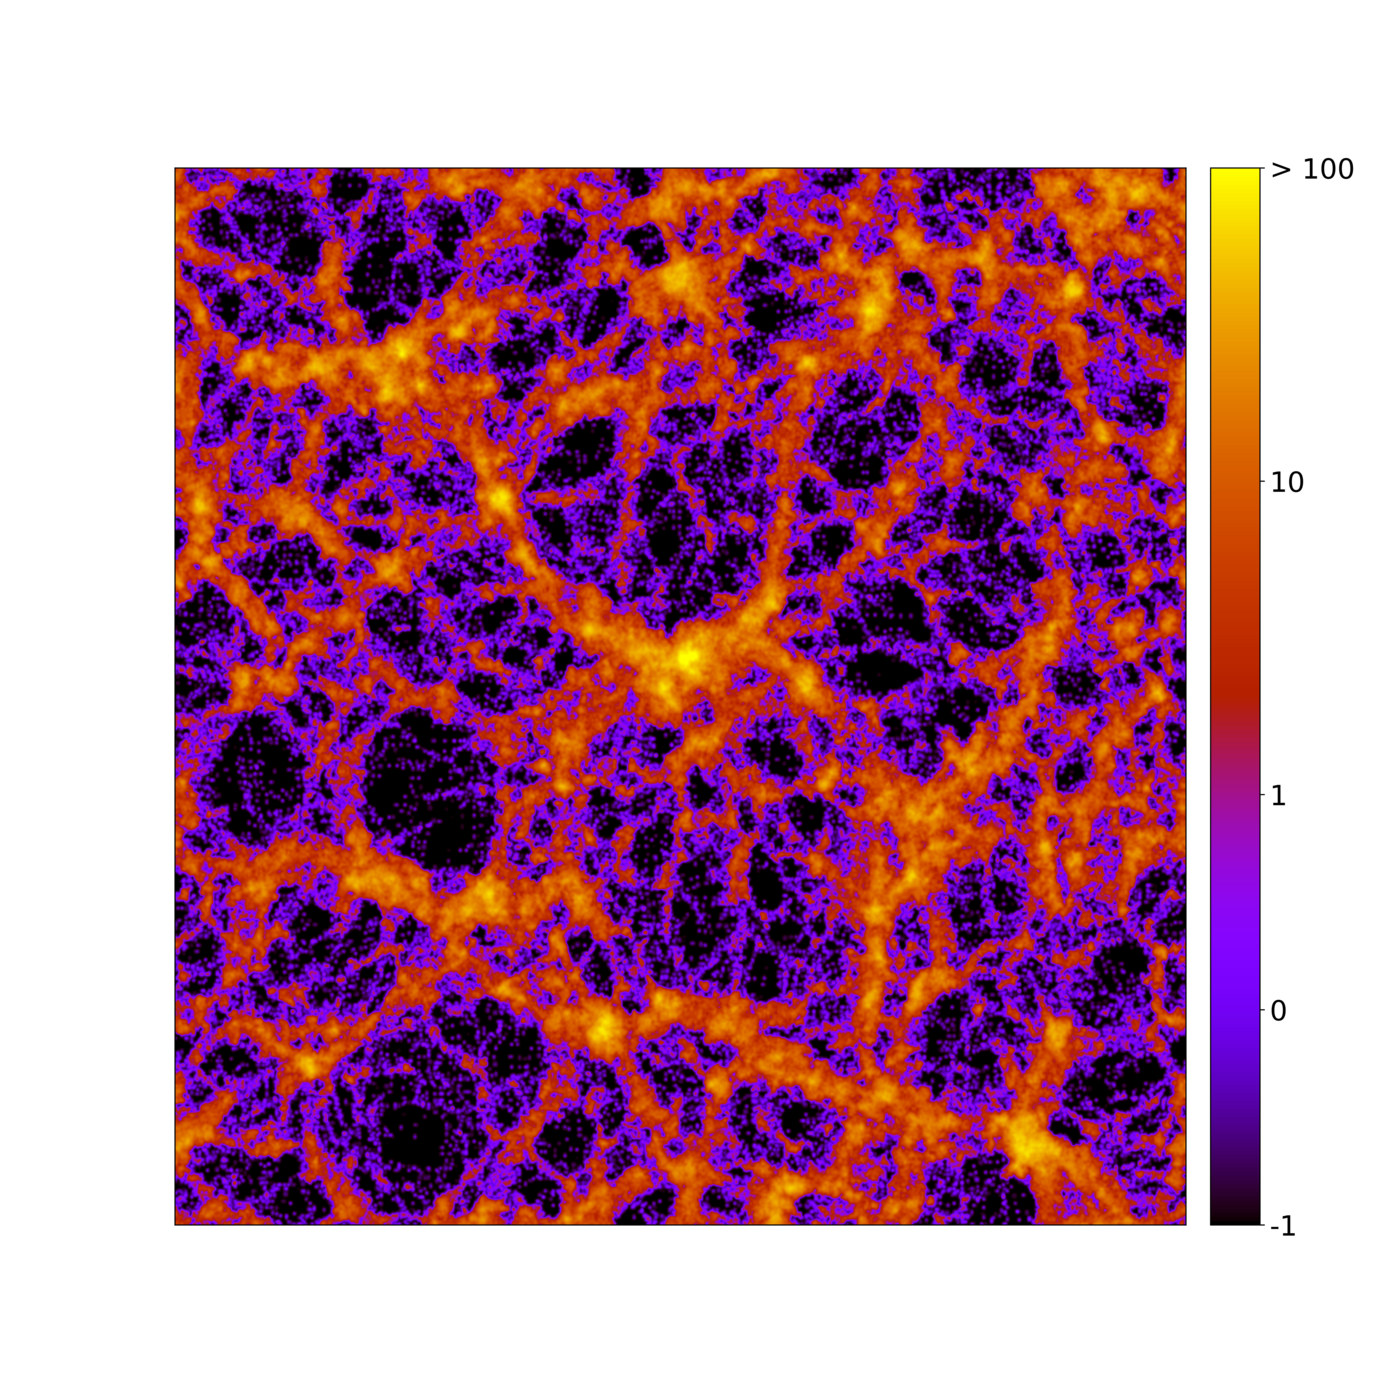
\includegraphics[width=1.0\linewidth]{{simulations_approx/dens/za_dens_512m_1p_1024M_200b_z0.00}.png}
			\caption{Zel`dovich approximation}
		\end{subfigure}%
		\begin{subfigure}{0.4\linewidth}
			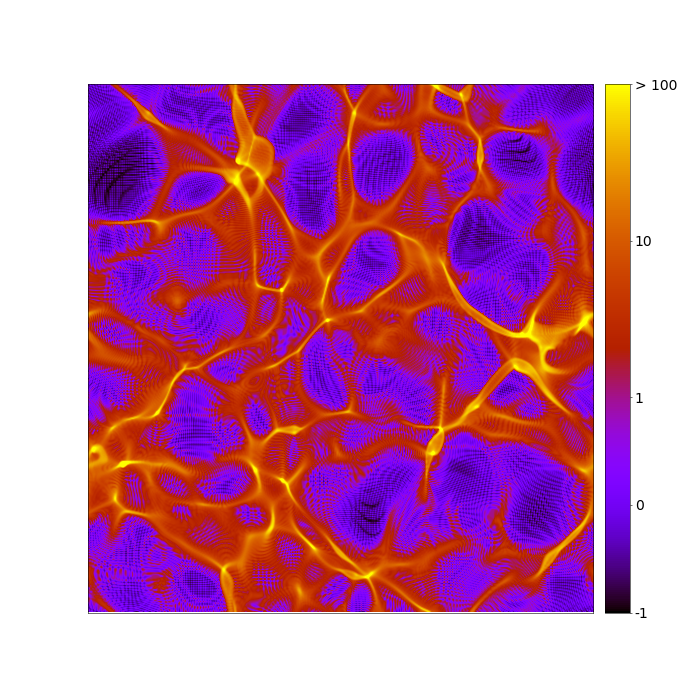
\includegraphics[width=1.0\linewidth]{{simulations_approx/dens/tza_dens_512m_1p_1024M_200b_z0.00}.png}
			\caption{Truncated Zel`dovich approximation}
		\end{subfigure}
		\begin{subfigure}{0.4\linewidth}
			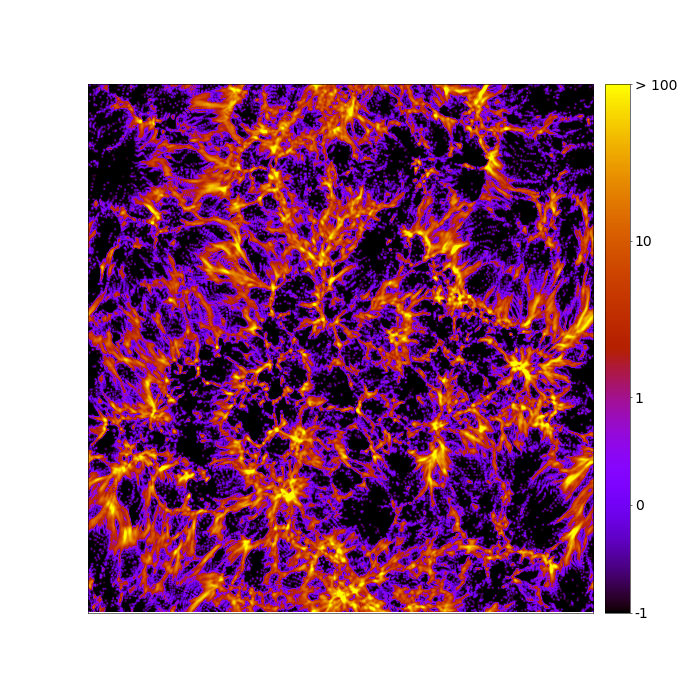
\includegraphics[width=1.0\linewidth]{{simulations_approx/dens/ff_dens_512m_1p_1024M_200b_z0.00}.png}
			\caption{Frozen-flow approximation}
		\end{subfigure}%
		\begin{subfigure}{0.4\linewidth}
			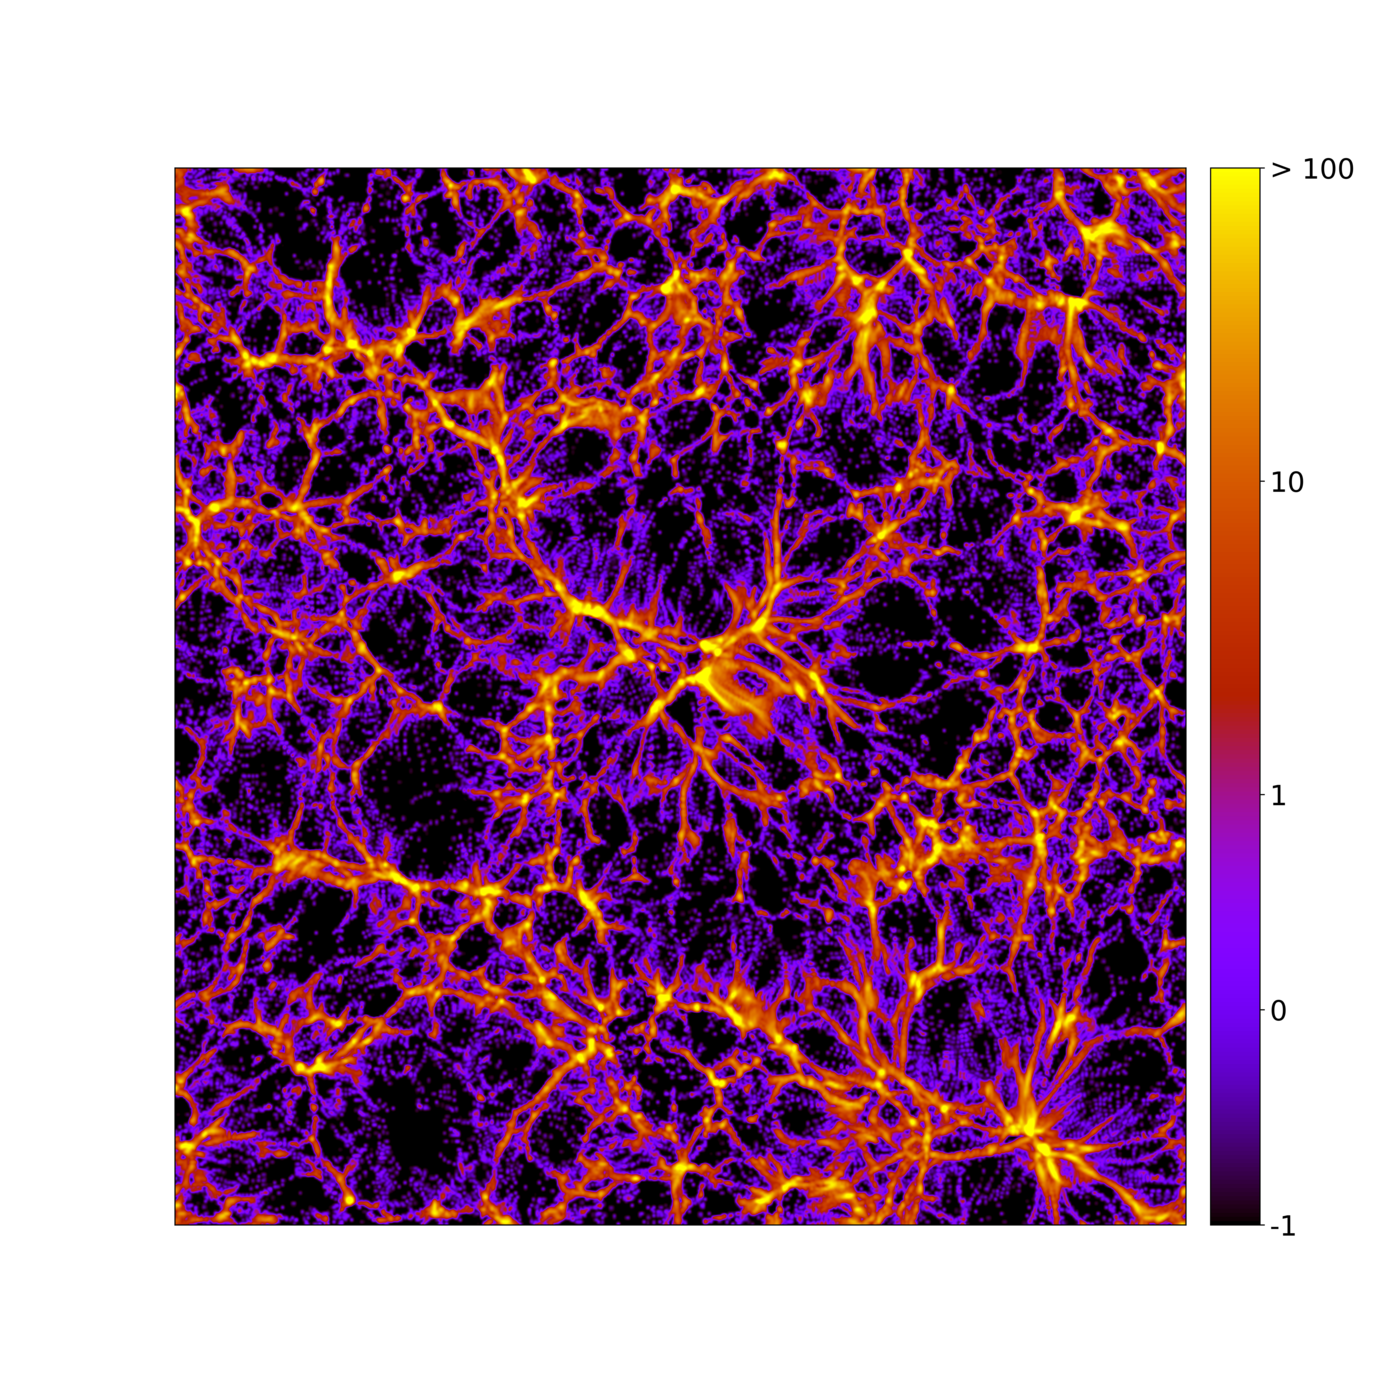
\includegraphics[width=1.0\linewidth]{{simulations_approx/dens/fp_dens_512m_1p_1024M_200b_z0.00}.png}
			\caption{Frozen-potential approximation}
		\end{subfigure}
		\begin{subfigure}{0.4\linewidth}
			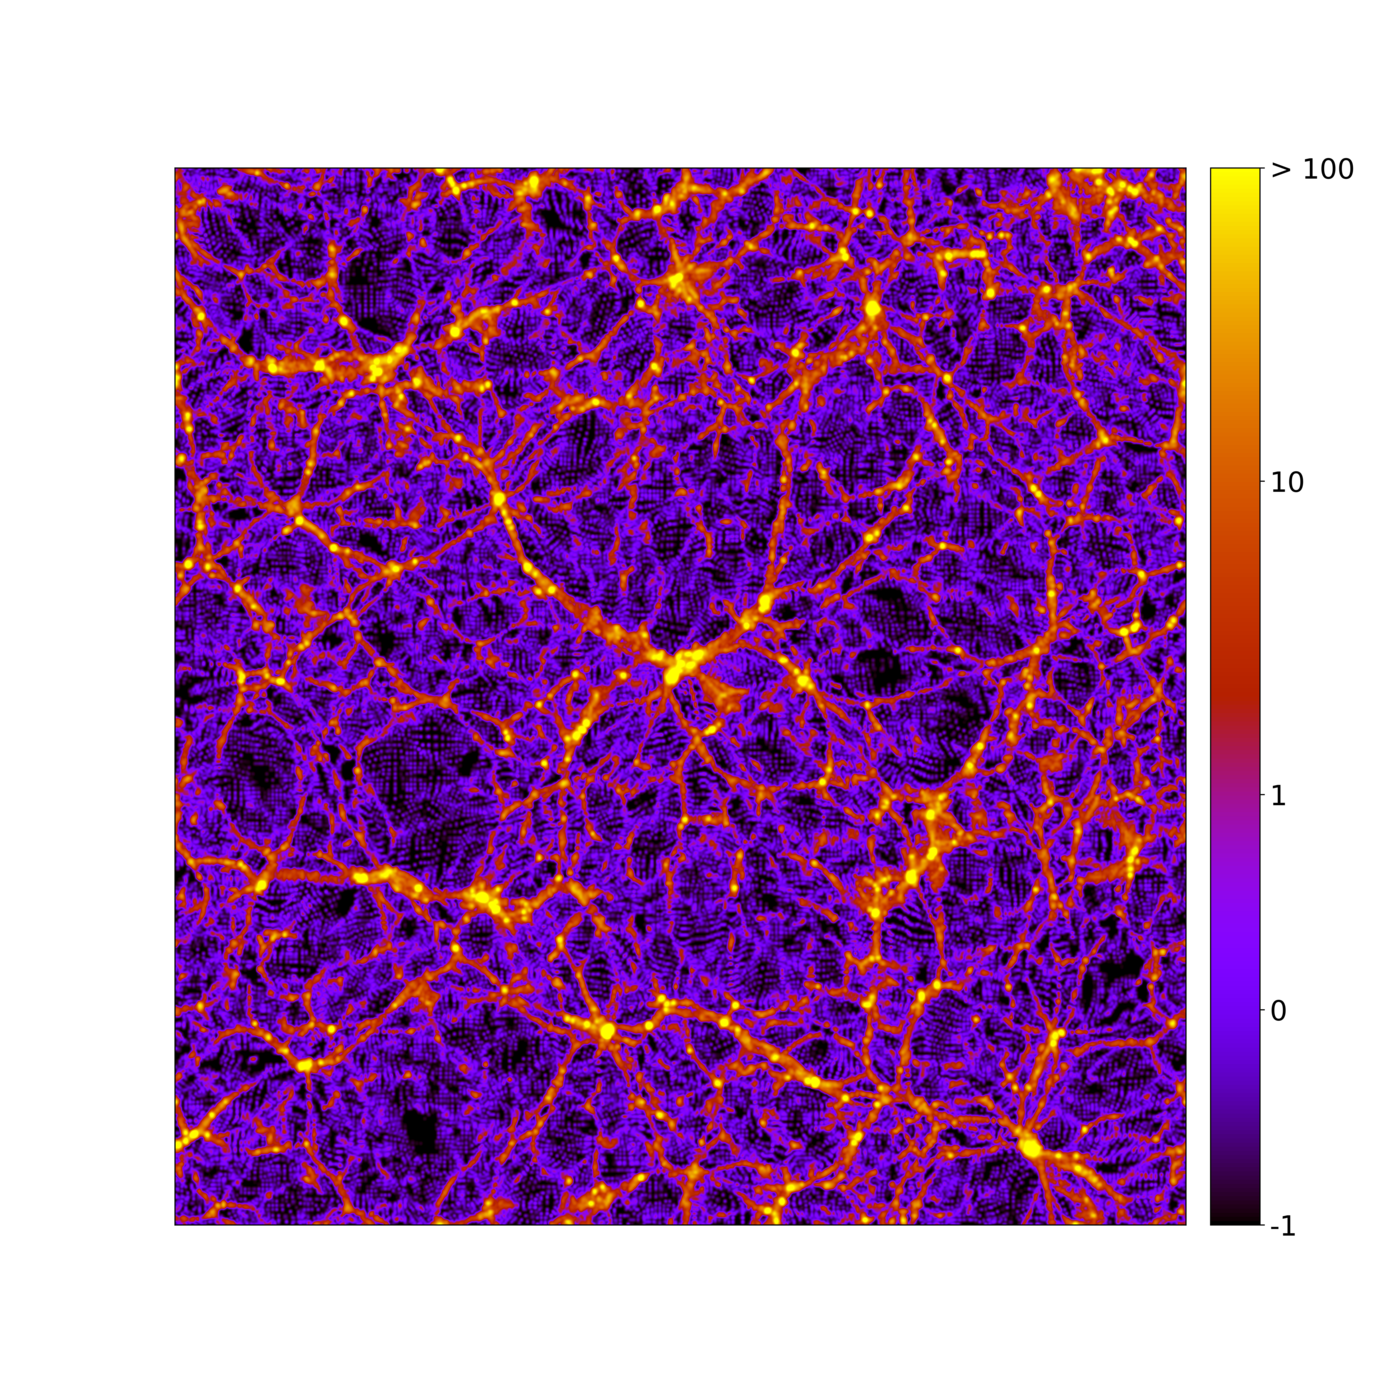
\includegraphics[width=1.0\linewidth]{{simulations_approx/dens/pm_dens_512m_1p_1024M_200b_z0.00}.png}
			\caption{PM simulation}
		\end{subfigure}
	\end{adjustwidth}
		\caption{Projected density field at redshift $z=0$ for the different approximations, all run with the same initial conditions. Each slice has a box-length of $200~\Mpch$ and is $1~\Mpch$ thick.}
		\label{fig:slice_dens_all}
\end{figure*}
\floatpagestyle{plain}
% } %% end afterpage


%%%%%%%%%%%%%%%%%%%%%%%%%%%%%%%%%%%%%%%%
% Approximation methods in modified gravity
%%%%%%%%%%%%%%%%%%%%%%%%%%%%%%%%%%%%%%%%
\section{Approximation methods in modified gravity}
Here we remind the basic chameleon equations we want to solve numerically. The non--linear Poisson equation
\eq{
\label{eq:cham_u_cp}
	\Delta\left(\chi/\chi_a\right)= C_\chi(a)\left[1+\delta-\left(\frac{\chi_a}{\chi}\right)^{1-n}\right]\,,
}
where
\eq{
	C_\chi(a)\equiv\frac{3H_0^2\Omega_m}{2\Phiscrz}a^{-3\frac{2-n}{1-n}}=\left(a\mu\Phiscra\right)^{-1}\,,
}
the linear solution
\eq{
\label{eq:chi_lin_x_cp}
	\chi(\mb x, a) = \chi_a(a)\left(1 + \frac{\Phi_G(\mb x, a)}{\Phiscra(a)} \right)\,.
}
the linear solution in $k-$space
\eq
{
\label{eq:chi_lin_k_cp}
	\hat{\chi}(k)=-\frac{\chi_a}{1-n}\frac{m^2}{m^2+k^2}\hat{\delta}(k) = -\frac{\beta\bar\rho_m}{\Mpl}\frac{\hat{\delta}(k)}{k^2+m^2}\,.
}
where the mass of the chameleon field is
\eq{
    \label{eq:chi_m_cp}
	m^2(a)\equiv\frac{1-n}{a\mu\Phiscra}\,,
}
and the screened solution inside massive objects
\eq{
	\chi=\frac{\chi_a}{\left(1+\delta\right)^{1/(1-n)}}\,.
	\label{eq:chi_bulk_cp}
}

When applying the approximation methods to the chameleon equations, we have three choices on how to arrive at an approximate solution:
\begin{enumerate}
\item \label{itm:lin_q} Purely linear prediction in $(\mb q, a)$-space, solution \eqref{eq:chi_lin_x_cp}

\item \label{itm:lin_k} Purely linear prediction in $(\mb k, a)$-space, solution \eqref{eq:chi_lin_k_cp}

\item \label{itm:nl_x} Non--linear prediction in $(\mb x, a)$-space, solution \eqref{eq:cham_u_cp}
\end{enumerate}

Choice \ref{itm:lin_q} means that there is no computational overhead and we can simply take the chameleon force to be $2\beta^2a^{-2}$ of the gravitational one. This method clearly overestimates the chameleon force at early times when the chameleon's Compton wavelength is short. This is because the solution \eqref{eq:chi_lin_x_cp} does not take into account the non-zero mass of the field.

A better choice is to use \ref{itm:lin_k} where the non-zero mass is incorporated. This solution adds relatively little computational overhead over normal gravity -- needing (at least) one Fourier transform and also extra storage. The overdensity $\delta(\mb k, a)$ is either the linearly evolved one, i.e. $\delta(\mb k, a) = D(a)\delta_0(\mb k)$, or we can compute $\delta$ at each time-step from the current positions of particles. This adds extra computation when assigning the mass of particles on the grid and one extra Fourier transform to get $\delta(\mb k, a)$. 
However, we cannot use \eqref{eq:chi_lin_k_cp} blindly to get a solution in real space as this linear approximation breaks down inside massive objects where we would get a negative solution. This effect is similar to a usage of linear evolution for $\delta$ where we can end up with regions where $\delta<-1$. We need to check if the resulting chameleon field is positive and fix it where it is not. We use the screening regime value \eqref{eq:chi_bulk_cp} to get a positive solution. We will refer to this prediction as pseudo-linear since it can address some effects of the screening mechanism.

The most expensive choice is \ref{itm:nl_x} where we must iteratively solve nonlinear equations. Unlike other methods this one can address the screening regime inside and near massive objects but at the cost of the most computational overhead.

%%%%%%%%%%%%%%%%%%%%%%%%%%%%%%%%%%%%%%%%
% Other approximations
%%%%%%%%%%%%%%%%%%%%%%%%%%%%%%%%%%%%%%%%
\section{Other approximations}
Approximations described previously are studied numerically in detail in the next chapter. Here we present few of the other approximations studied in the past or used today.

\subsection{Adhesion approximation}
The adhesion approximation was introduced in \textcite{1989MNRAS.236..385G}. To study the evolution of density inhomogeneities they used model of non--linear diffusion (Burger`s equation), that gives an approximate description of the growth of structures at the advanced non--linear stage of gravitational instability.

To overcome problems of ZA with shell-crossing they propose a solution of ``sticking articles.'' Particles move according to ZA until they ran into one another. Then they move together, with the velocity conserving momentum. This model can be described mathematically by inserting the viscous term into equations of motion, simulating attractive forces of gravity
\eq{
	\dddd{\mb u\AAP}{a}=\nu\partpart{^2\mb u}{\mb x^2}\,.
}
The Burger`s equation has an analytical solution which can be used to study formation of structures. For more information regarding the adhesion approximation see  also \textcite{1990MNRAS.247..260W,1994ApJ...428...28M}.

\subsection{Stable clustering}
It was proposed by \textcite{1974ApJ...189L..51P} that clustering in the very non--linear regime might be understood by assuming that regions of high--density contrast undergo virialization and subsequently maintain a fixed proper density, hence stable clustering. The correlation function for a population of such systems would then simply evolve according to
\eq{
	\xi(r,a)\propto1/\bar\rho\propto a^3\,.
}
\textcite{1991ApJ...374L...1H} developed a method for interpolating between linear theory on large scales and the non--linear predictions of the stable clustering hypothesis on small scales. They showed that the non--linear volume-averaged two-point correlation function could be parameterized by a simple function of the linear correlation function
\eq{
	\bar\xi_{NL}=f(\bar\xi_{L})\,,
}
where the functional form of $f$ can be derived from the spherical top-hat model without any shell-crossing. For the linear regime $\bar\xi_{L}\ll1$, $f(y)=y$, and for non--linear $\bar\xi_{L}\gg1$, $f(y)=y^{3/2}$. For more information regarding the stable clustering see  also \textcite{1996MNRAS.280L..19P,2003MNRAS.341.1311S}.
\subsection{Lagrangian perturbation theories of higher--orders}
Success of ZA, the first--order Lagrangian perturbation theory (LPT), has motivated studies of higher--order corrections \parencite[see e.g.][]{10.1093/mnras/264.2.375,2002PhR...367....1B,2010MNRAS.403.1859J,2014ApJ...788...63S}. In the Lagrangian description, the spatial coordinates are transformed through the displacement vector $\Psi$ as
\eq{
	\mb x = \mb q + \Psi(a, \mb x)\,.
}
In LPT, this displacement vector field is expanded in a perturbation series in the linear growth function $D$ in Fourier space. Density perturbations $\delta$ are described as a function of the displacement vector through conservation of mass. This Lagrangian picture is intrinsically non--linear in the density field, and a small perturbation in Lagrangian fluid element paths carries a considerable amount of non--linear information about the corresponding Eulerian density and velocity fields. Different variants of LPT -- third order LPT (\cite{10.1093/mnras/264.2.375}), Truncated LPT (\cite{10.1093/mnras/260.4.765}), Augmented LPT (\cite{10.1093/mnrasl/slt101}), MUSCLE (\cite{10.1093/mnrasl/slv141}) -- have been tested against particle-mesh code COLA (\cite{2013JCAP...06..036T}) in \cite{2017JCAP...07..050M}, see \autoref{fig:app_compare}.

\begin{figure}[!htb]
    \centering
    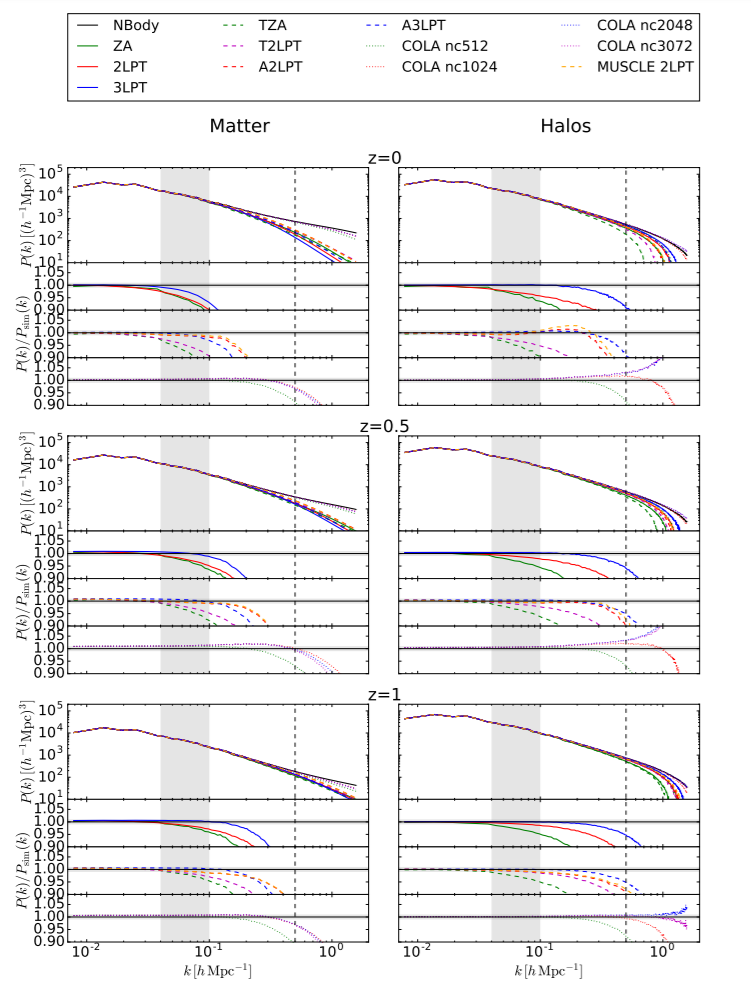
\includegraphics[width=0.9\textwidth]{cosmo_evol/app_compare.png}
    \caption{Power spectrum at $z = 0,\ 0.5$ and $1$ (top, middle and bottom panels, respectively) in real space and ratio with the \nbody’s one for the matter field (left panels) and for the halo catalogues (right panels). The vertical dashed line locates the $k = 0.5\hMpc$ where the one-halo term becomes significant. The vertical shaded area locates the region of the BAO peak, while the horizontal one locates the 1\% accuracy region.  \textit{Note:} Reprinted from \textcite{2017JCAP...07..050M}.}
    \label{fig:app_compare}
\end{figure}
\chapter{Simulations with Approximation Methods}

\section{Motivation}

\section{Results}

\subsection{Power spectrum}

\subsection{Effective redshift}

\subsection{Correlation function}

\section{Chameleon results}
% % \chapter{Simulations with GADGET}

\section{GADGET}

\section{Results}

\subsection{Code Comparison}

\subsection{Power spectrum}

\subsection{Effective redshift}

\subsection{Correlation function}

\subsection{Halo mass function}

\section{Chameleon results}

% \chapter{Cosmological Surveys}
\label{chpt:cosmo_surveys}
There are many projects and missions which study properties of the dark energy, either as a main scientific goal, or as a complementary program. Among the big surveys are e.g. Sloan Digital Sky Surveys (SDSS, \cite{SDSS}) which aims to create the most detailed three-dimensional maps of the Universe. From the beginning of regular surveys in 2000 till 2014 there were seven finished surveys in total (SDSS-I/II results \cite{SDSS_I_II}, SDSS-III results \cite{BOSS_results}), while there are three ongoing surveys from 2014 (SDSS-IV, \cite{2017AJ....154...28B}) and a planned panoptic spectroscopic survey (SDSS-V, \cite{2017arXiv171103234K}) which will start collecting data in summer 2020. Other surveys are e.g. Wilkinson Microwave Anisotropy Probe (WMAP, \cite{WMAP}, results \cite{WMAP_results}); Planck (\cite{planck}, results \cite{planck_cosm}). There are also several planned surveys almost ready to start collecting data -- Euclid \parencite{euclid}, LSST \parencite{lsst} or W-FIRST \parencite{WFIRST_report}.

Some parts of this chapter are based on the author`s work \textcite{mastersthesis_vrastil}.
\section{BOSS}
The Sloan Digital Sky Survey`s (SDSS-III) Baryon Oscillation Spectroscopic Survey (BOSS) is a six-year program (Fall 2009 -- Spring 2014)  that uses the wide-field 2.5-m telescope at Apache Point Observatory, see \autoref{fig:sdss_tele}. The BOSS is designed to measure the scale of baryonic acoustic oscillations (BAO, see \autoref{sec:bao}) in the clustering of matter over a larger volume than the combined efforts of all previous spectroscopic surveys of large-scale structures. BOSS uses 1.5 million luminous galaxies to measure BAO to redshifts $z<0.7$. Observations of neutral hydrogen in the Ly$\alpha$ forest in more than 150,000 quasar spectra constrain BAO over the redshift range $2.15 < z < 3.5$ \cite{BOSS}.
\begin{figure}[ht]
    \centering
    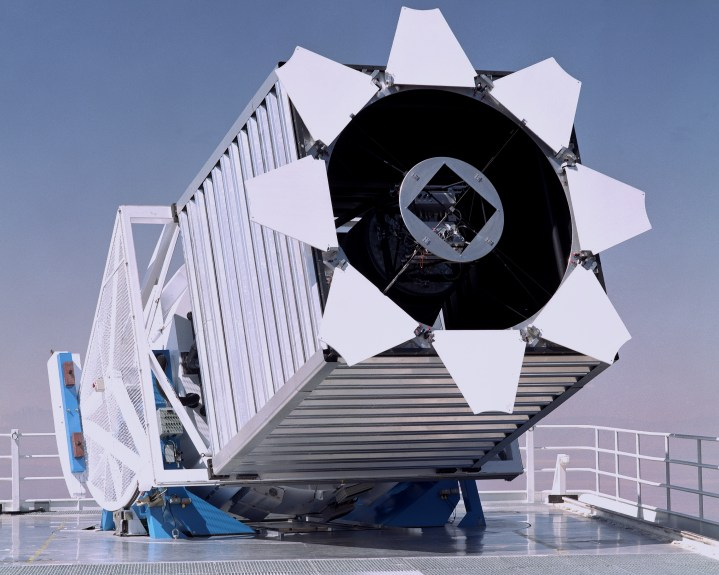
\includegraphics[width=0.9\textwidth]{cosmo_surveys/SDSS_telescope_new.jpg}
    \caption{Sloan Foundation 2.5m Telescope.}
    \label{fig:sdss_tele}
\end{figure}

There are two double spectrographs, each covering the wavelength range 361 nm -- 1014 nm with resolution $R=\lambda/\Delta\lambda$ ranging from 1300 at the blue end to 2600 at the red end.  Both spectrographs have a red channel with a 4k $\times$ 4k, 15\um  pixel CCD from Lawrence Berkeley National Laboratory (LBNL). Both spectrographs have a blue channel with a 4k $\times$ 4k, 15\um  pixel CCD from  e2v. The instrument is fed by 1000 optical fibers (500 per spectrograph), each subtending 2\arcsec\ on the sky.

Using the acoustic scale as a physically calibrated ruler, BOSS determines the angular diameter distance with a precision of 1\% at redshifts $z = 0.3$ and $z = 0.57$ using the distribution of galaxies and measurements of $H(z)$ to 1.8\% and 1.7\%  at the same redshifts. At redshifts $z\sim2.5$ the  angular diameter distance and $H\mins(z)$ is measured to an accuracy of 1.9\% using Ly$\alpha$ forest.

BAO measurements with the CMB-calibrated physical scale of the sound horizon and SN data yields of $H_0=(67.3\pm1.1)$ \unith\ with 1.7\% precision \cite{BOSS_results}, see \autoref{fig:boss_Hz}. This measurement assumes standard pre-recombination physics but is insensitive to assumptions about dark energy or space curvature. When we allow more general forms of evolving dark energy, the BAO+SN+CMB parameter constraints are always consistent with flat \LCDM\ values at $1\sigma$. While the overall $\chi^2$ of model fits is satisfactory, the Ly$\alpha$ forest BAO measurements are in moderate $(2-2.5\sigma)$ tension with model predictions. Models with early dark energy that tracks the dominant energy component at high redshift remain consistent with expansion history constraints, and they yield a higher $H_0$ and lower matter clustering amplitude, improving agreement with some low-redshift observations.
\begin{figure}[ht]
    \centering
    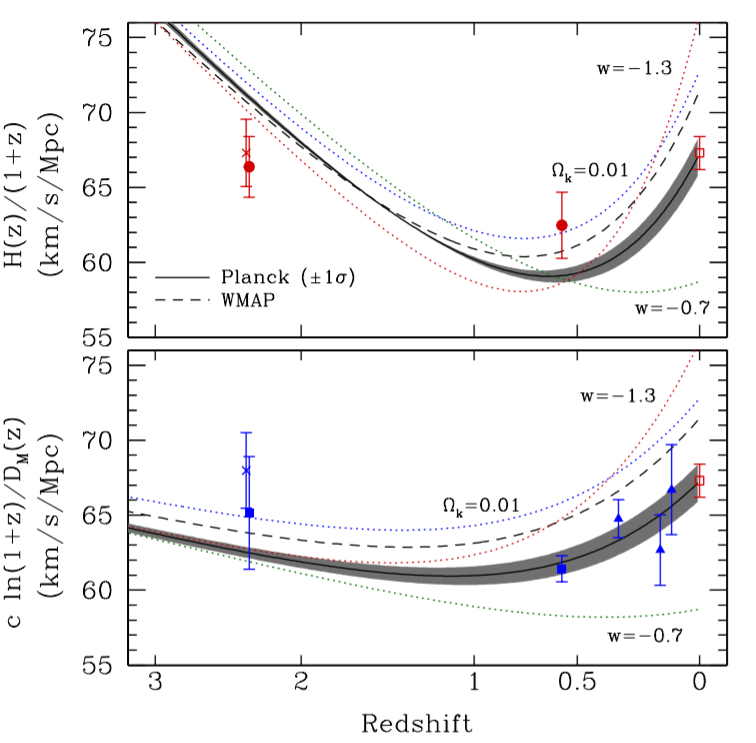
\includegraphics[width=0.9\textwidth]{cosmo_surveys/boss_Hz.png}
    \caption{BAO measurements and model predictions of \(H(z)\) and \(D_M(z)\) as a function of redshift, with physically informative scalings. The top panel shows \(H(z)/(1+z)\), the proper velocity between two objects 1 comoving Mpc apart. The bottom panel shows \(c\ln{(1+z)}/D_M(z)\), a scaling that matches a constant line \(H(z)=(1+z)H_0\) in the top panel to the same constant line in the bottom panel for a flat universe. Filled circles and squares show the BOSS CMASS and Ly$\alpha$ forest measurements of \(H(z)\) and \(D_M(z)\), respectively; we show the Ly$\alpha$ forest quasar cross-correlation as crosses to distinguish from the Ly$\alpha$ forest auto-correlation measurments. Filled triangles in the bottom panel show the BOSS LOWZ and MGS measurements of \(D_V (z)\) converted to \(D_M(z)\). Open squares show the value of \(H_0 = 67.3\pm1.1\) \unith determined from the combination of BAO and SN Ia data. The grey swath in both panels is the prediction from the Planck \LCDM\ cosmology including \(1\sigma\) parameter errors; in the top panel, one can easily see the model transition from deceleration to acceleration at \(z\approx0.6\). The dashed line shows the \LCDM\ prediction using the best-fit WMAP parameters, which has lower \(\Omega_mh^2\). Dotted curves show models that match the best-fit Planck values of \(\omega_{cb}\), \(\omega_{b}\), and \(D_M(1090)/r_d\) but have \(\Omega_k = 0.01\) (blue), \(w = -0.7\) (green), or \(w = -1.3\) (red). The \textit{x}-axis is set to \(\sqrt{1+z}\) both for display purposes and so that a pure matter universe \((\Omega_m = 1)\) appears as a decreasing straight line on the top panel. \textit{Note:} Reprinted from \textcite{BOSS_results}.}
    \label{fig:boss_Hz}
\end{figure}
\section{eBOSS}
The Extended Baryon Oscillation Spectroscopic Survey (eBOSS, \cite{2016AJ....151...44D}) is the new cosmological survey within a SDSS-IV six-year program started in 2014 July. eBOSS will conduct novel cosmological observations of galaxies, and in particular quasars, using the same 1000-fiber optical spectrographs as those in BOSS at Apache Point Observatory. These observations will be conducted simultaneously with the Time Domain Spectroscopic Survey (TDSS, \cite{2015ApJ...806..244M}) designed for variability studies and the Spectroscopic Identification of eROSITA Sources (SPIDERS, \cite{2010SPIE.7741E..1NF}) program designed for studies of X-ray sources.

eBOSS will map the large-scale-structures over the relatively unconstrained redshift range $0.6<z< 2.2$, see \autoref{fig:eboss} for comparison with BOSS range. eBOSS will expand the selection of luminous red galaxies (LRG) beyond that probed by BOSS and obtain better than a $1.0\%$ precision distance estimate when combined with the $z > 0.6$ tail of the BOSS galaxy population. With observations of a new sample of emission line galaxies (ELG) eBOSS will produce a $2.0\%$ precision distance estimate at higher redshifts. eBOSS will obtain a $1.8\%$ precision distance estimate in the redshift range $0.9 < z < 2.2$ using quasars that have luminosities and areal densities well-suited to sensitivity of the BOSS spectrographs. Finally, eBOSS will sharpen the BOSS Ly$\alpha$ forest measurements by a factor of $1.44$ with a new selection of $z > 2.1$ quasars, providing stronger leverage on the history of dark energy.
\begin{figure}[ht]
    \centering
    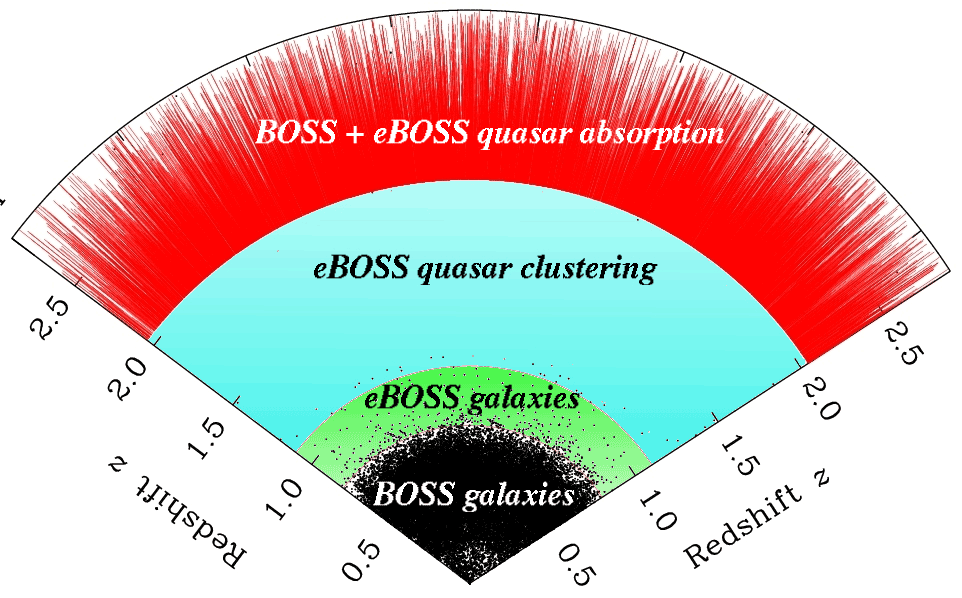
\includegraphics[width=0.9\textwidth]{cosmo_surveys/pie_boss_eboss_marked.png}
    \caption{Planned eBOSS coverage of the Universe.}
    \label{fig:eboss}
\end{figure}

With four classes of spectroscopic targets (LRG, ELG, quasar, Ly$\alpha$ forest quasar), eBOSS will enable the first high precision distance measurements in the epochs when dark energy emerged as the dominant dynamical component of the Universe. In addition to BAO distance measurements, eBOSS will provide new tests of GR on cosmological scales through redshift-space distortions (RSD), new tests for non-Gaussianity in the primordial density field, and new constraints on the summed mass of all neutrino species.
\section{DES}
\label{DES}
The Dark Energy Survey (DES) is designed to probe the origin of the accelerating universe and to help uncover the nature of dark energy by measuring the \mbox{14-billion-year} history of cosmic expansion with high precision. DES is an optical near infrared survey of 5000 deg\sq\ of the South Galactic Cap up to absolute magnitude $r\sim24$ in $grizy$ spectrum. DES`s instrument consists primarily of a new camera, Dark Energy Camera (DECam), specifically designed to be sensitive to the highly redshifted light from distant galaxies. DECam is mounted on a classic telescope, the Blanco 4-m telescope at the Cerro Tololo Inter-American Observatory (CTIO) in La Serena, Chile. The imaging system is supported by a combination of microwave and optical data links that will provide the recorded data to the survey members. Starting in August of 2013 and continuing for five years, DES has begun to survey a large swath of the southern sky out to vast distances in order to provide new clues to this most fundamental questions \cite{DES}.

\begin{figure}[ht]
    \centering
    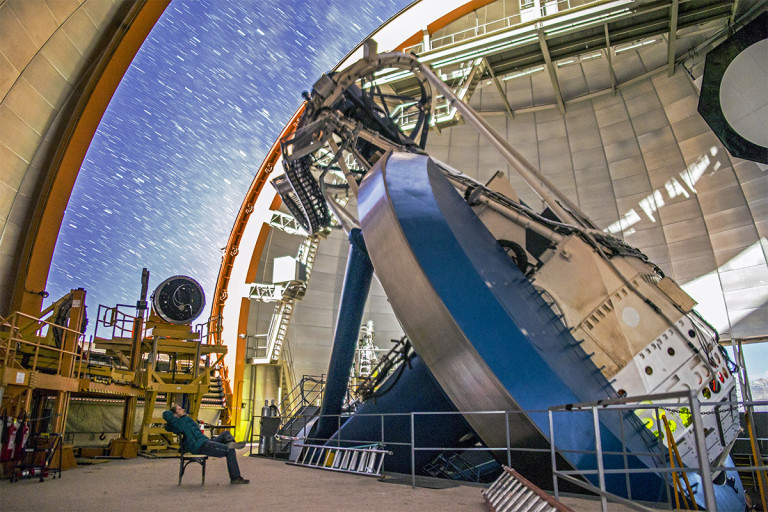
\includegraphics[width=0.9\textwidth]{cosmo_surveys/des.jpg}
    \caption{DESCam operating at night, while an observer watches.}
    \label{fig:des}
\end{figure}
The survey data allow to measure the dark energy and dark matter densities and the dark energy equation of state through four independent methods: galaxy clusters (counts and spatial distributions at $0.1<z<1.3$), weak gravitational lensing tomography (on several redshift shells to $z\sim1$), galaxy angular clustering, and supernova distances (at $0.3<z<0.8$).

The main tool is the DECam, 74 2k $\times$ 4k 570 Mpx digital camera built at Fermilab in Batavia. It provides a 2.2\textdegree\ field of view image at 0.27\arcsec/pixel. It covers wavelength range 400--1100 nm with five filters $(grizy)$. The electronics will allow an entire digital image to be read out and recorded in 17 seconds, time that it takes the telescope to move to its next viewing position.

From the first two years of observation a mass map from weak gravitational lensing shear measurements over 139 deg\sq\ has been reconstructed \cite{DES_mass}. There is a good agreement between the mass map and the distribution of massive galaxy clusters identified using a red-sequence cluster finder. These measurements are consistent with simulated galaxy catalogs based on \LCDM\ \nbody\ simulations, suggesting low systematics uncertainties in the map.

In \textcite{2019PhRvL.122q1301A} the DES collaboration presented their cosmological constraints for \wCDM: $\Omega_m=0.300^{+0.023}_{-0.021}$, $\Omega_b=0.064^{+0.013}_{-0.009}$, $\Omega_\Lambda=0.700^{+0.021}_{-0.023}$, $w=-0.80^{+0.09}_{-0.11}$ and $\sigma_8=0.786^{+0.029}_{-0.019}$. Constraints on the dark energy equation of state $w$ and $\Omega_m$ for \wCDM\ are also shown in \autoref{fig:des_res}.

\begin{figure}[ht]
    \centering
    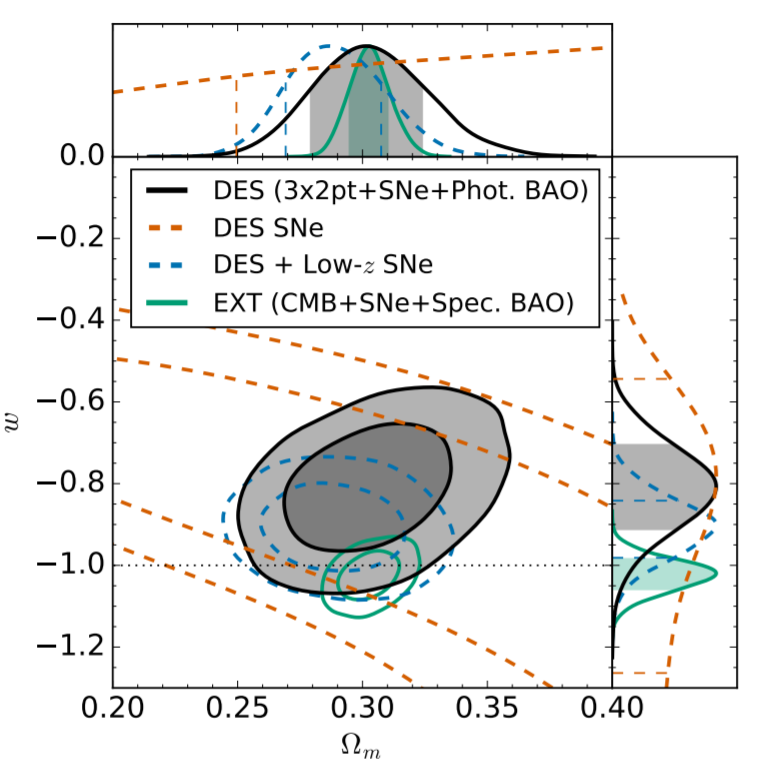
\includegraphics[width=0.7\textwidth]{cosmo_surveys/DES_constraints.png}
    \caption{Constraints on the dark energy equation of state $w$ and $\Omega_m$ in a \wCDM\ model with fixed curvature $(\Omega_k=0)$ and marginalized neutrino mass density. They compared constraints from the DES data alone (black contours) to the best available external data (green contours), but also showed the impact of including a lowredshift SNe Ia data set (Low-$z$) to anchor the DES SNe Ia (blue contours). Each component of the DES analysis was fully blinded. Reprinted from \textcite{2019PhRvL.122q1301A}.}
    \label{fig:des_res}
\end{figure}
\section{Euclid}
Euclid is an ESA (European Space Agency) high-precision space mission in ESA`s Cosmic Vision 2015--2025 scientific programme designed to map the geometry and evolution of the universe and to study properties of dark matter and dark energy. Its primary goal is to place high accuracy constraints on dark energy, dark matter, gravity and cosmic initial conditions using two independent cosmological probes -- weak gravitational lensing and baryonic acoustic oscillation -- out to redshift $z\sim2$. Galaxy clusters and the Integrated SachsWolfe effect will be used as secondary cosmological probes. Along with these tasks will Euclid`s visible and near infrared imaging and spectroscopy of the entire extragalactic sky produce legacy science for various fields of astronomy, e.g. galaxy evolution, large-scale structures or the search for high-redshift objects. The Euclid mission has been adopted with the mission`s time--frame for liftoff starting in mid-2022 from the Guiana Space Centre, Europe`s Spaceport in French Guiana. Overview of the Euclid system design and scientific requirements can be found in \cite{2011arXiv1110.3193L}.
\begin{figure}[ht]
    \centering
    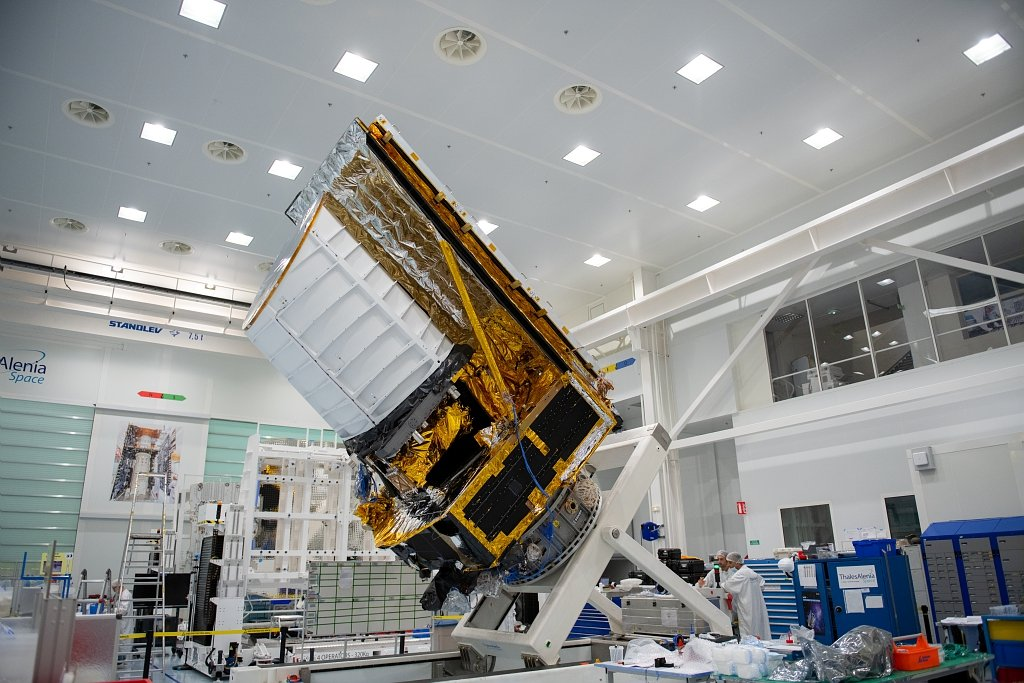
\includegraphics[width=0.9\textwidth]{cosmo_surveys/euclid.jpg}
    \caption{Structural and thermal model of the Euclid satellite.}
    \label{fig:euclid}
\end{figure}
% \subsection{The Euclid Consortium}
% The Euclid Consortium (EC) is an organisation that brings together teams of researchers in theoretical physics, particle physics, astrophysics and space astronomy, and also engineers, technicians, and management and administrative staffs working in public research laboratories and contributing to the Euclid mission. Together with the European Space Agency (ESA) and aerospace industry they are part of the Euclid Collaboration. The EC has been selected by ESA in June 2012 as the single official scientific consortium having the responsibility of the scientific instruments, the production of the data and of leading the scientific exploitation of the mission until completion. It is funded by national space agencies and national research organizations and led by the Euclid Consortium Lead (ECL) and a Euclid Consortium Board (ECB). The ECL and ECB are the primary contact points with ESA and with the Euclid Consortium members.

\section{Vera C. Rubin Observatory}
The Vera C. Rubin Observatory project, previously known as the Large Synoptic Survey Telescope, will conduct the 10-year Legacy Survey of Space and Time (LSST, \cite{lsst}). LSST is a ground-based telescope being built in northern Chile on the Cerro Pach\'{o}n mountain in the northern Chilean Andes. The system will produce a 6-band (300 -- 1100 nm) wide-field deep astronomical survey over 20,000 deg\sq\ of the southern sky. Combining the wide field of view with short exposures, the LSST will take more than 800 images each night and cover the whole observable sky twice each week. Each patch of the sky will be visited about 1000 times during ten years. The LSST will provide an unprecedented depth (single-visit 24.5 mag, co-added 27.5 mag) and unique details of the Universe while producing 30 terabytes of data nightly. This data will be used for locating dark matter and to characterize the properties of the dark energy. Other major tasks for the LSST will be detecting and tracking potentially hazardous asteroids or studying the structure of the Milky Way. The project is in the construction phase and will begin its full science operations in 2022. The exterior of the summit facility building is nearly complete, see \autoref{fig:lsst_site}. Inside, major components of the telescope have begun to arrive from their places of manufacture around the globe, including the mirror washing and coating equipment, and the Secondary Mirror (M2) and its support system.

On January 6, 2020, it was announced that the LSST will be named the NSF (National Science Foundation) Vera C. Rubin Observatory (Rubin Observatory) after an astronomer who provided important evidence of the existence of dark matter. NSF also announced on January 6, 2020, that the telescope at the Rubin Observatory will be named the Simonyi Survey Telescope in recognition of the significant private donation made through the Corporation early in the construction phase in support of the design, development, and fabrication of the telescope`s primary mirror.
\begin{figure}[ht]
    \centering
    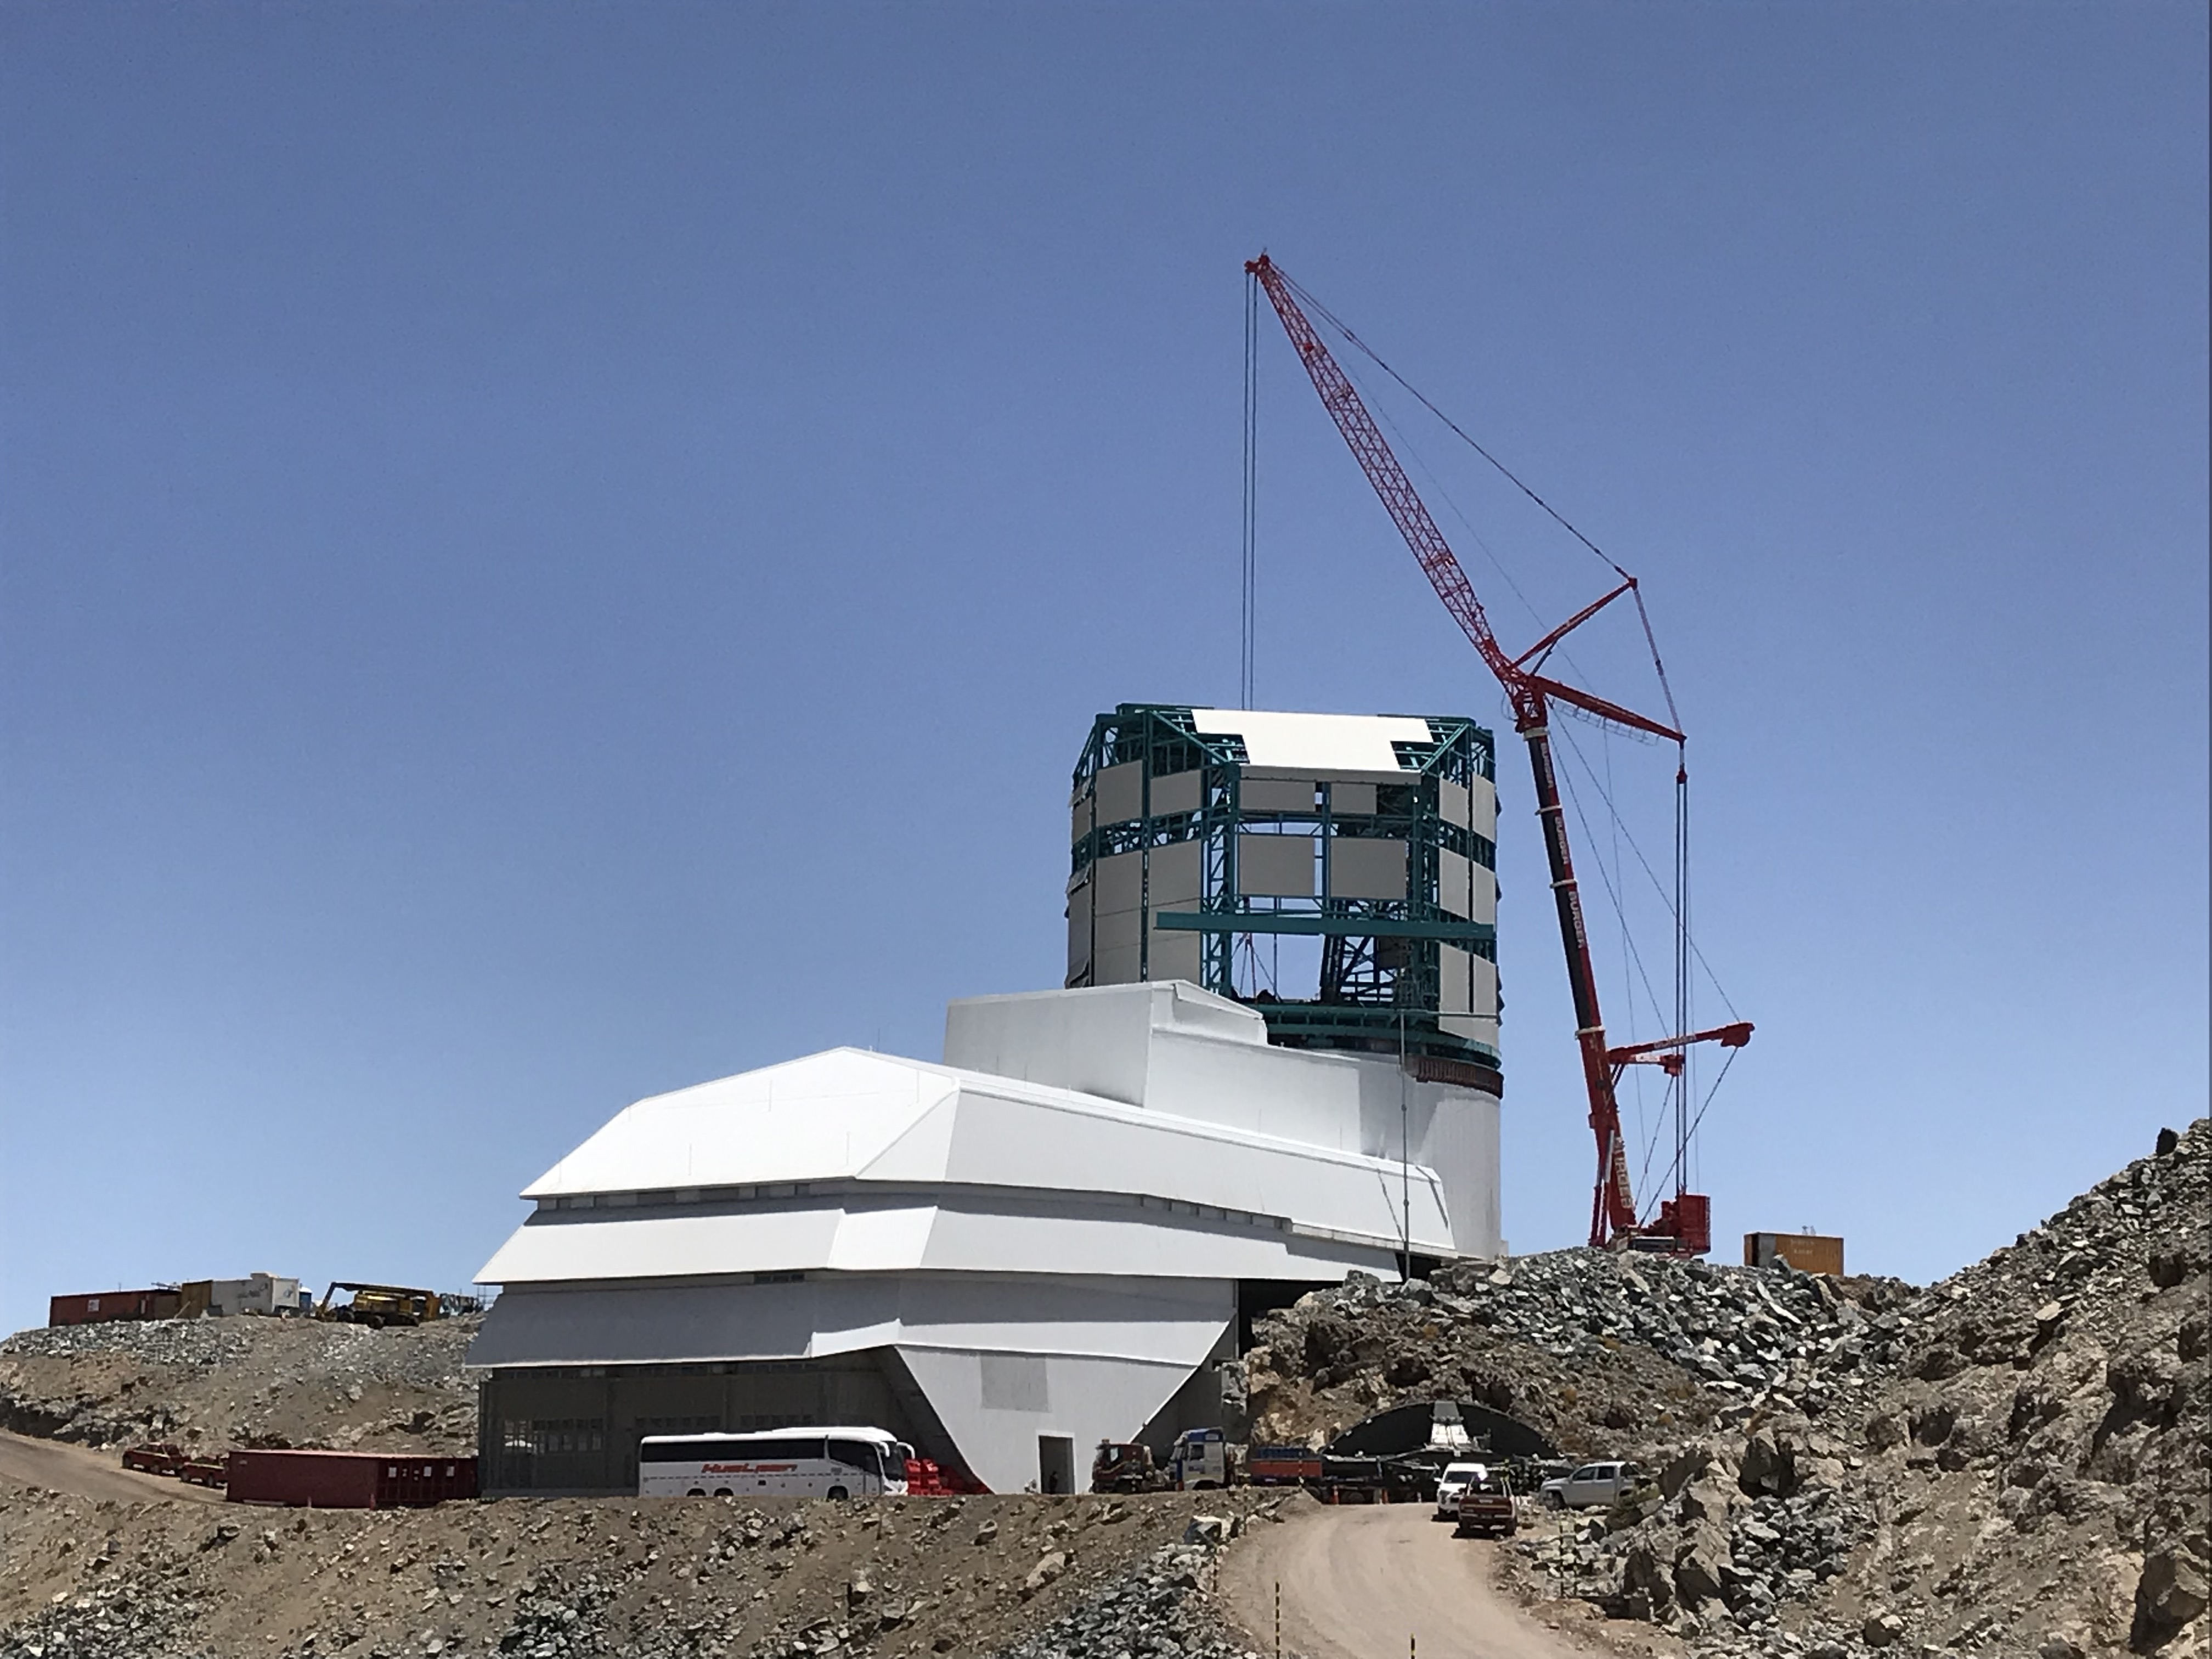
\includegraphics[width=0.9\textwidth]{cosmo_surveys/lsst_site.jpg}
    \caption{Construction on the Vera C. Rubin Observatory. Most of the large pieces of equipment have arrived on the summit, and installation of the Telescope Mount Assembly (TMA) began in early 2020. Credit: LSST Project/NSF/AURA}
    \label{fig:lsst_site}
\end{figure}

The LSST Data Management (DM) is responsible for creating the software, services and systems which will be used to produce LSST's data products. DM is required to generate and process a set of data products and to make them available to scientists and the public \parencite{LSST_DM}.

\subsection{Telescope and camera}
The LSST telescope consists of three aspheric mirrors -- an 8.4-m primary M1, a 3.4-m convex secondary M2 (the largest convex mirror ever made), and a 5.0-m tertiary M3. The primary mirror is highly annular having an outer clear aperture of 8.36 m and an inner diameter of 5.12 m, giving an effective collecting area of a 6.67-m filled aperture. The camera body and its associated readout electronics are located in the 1.8-m diameter hole in the secondary mirror.  The hole in the tertiary mirror is used to mount equipment for the maintenance of the LSST optical alignment. The primary and tertiary mirrors form a continuous surface without any vertical discontinuities. The M1-M3 monolith (see \autoref{fig:lsst_m1m3}) was completely formed and polished in February 2015 and in early 2019 it was shipped to the summit facility on Cerro Pach\'{o}n.
\begin{figure}[ht]
    \centering
    \includegraphics[width=0.9\textwidth]{cosmo_surveys/lsst_m1m3.jpg}
    \caption{The LSST Primary/Tertiary Mirror (M1M3) in the Richard F Caris Mirror Lab at the University of Arizona for optical testing. In May, 2019, the mirror reached its new home in the Andes Mountains of Northern Chile. Credit: LSST Project/NSF/AURA}
    \label{fig:lsst_m1m3}
\end{figure}

The LSST camera with size of 1.6 meters by 3 meters and weight of 2800 kilograms will be the largest digital camera ever constructed. It will produce data of extremely high quality with minimal downtime and maintenance. It is a large-aperture, wide-field optical (0.3--1 \um) imager designed to provide a 3.5\textdegree\ field of view with sampling better than 0.2\arcsec. The image surface is flat with a diameter of approximately 64 cm. Used detectors are 16 Mpixel silicon detectors providing a total of approximately 3.2 Gpixels with read out in 2 sec (15 sec integration). The camera has 6 filters ($ugrizy$) and is located in the middle of the telescope.

The focal plane consists of 189 arrays ($\sim$16 cm\sq\ each, 3200 cm\sq\ focal plane) of 4k$\times$4k CCDs which should ensure wide field of view while filling the focal plane without any large gaps (less than few hundred \um) -- the fill factor is 93\%. High resistivity silicon substrate and high applied voltages with small pixel size will produce low point spread function (PSF $\ll0.7$\arcsec). Other focal plane requirements include high quantum efficiency (QE) from 320 to 1080 nm, fast f/1.23 focal ratio, high throughput fast readout (2 sec) or low read noise \parencite{2017JInst..12C3017A}.


\subsection{Dark Energy Science Collaboration}
The LSST Project Team has been assembled to design and build the telescope, camera, and data management systems but it is not a scientific collaboration in the usual sense. While scientists working on the LSST Project are interested in the scientific questions that LSST data can address, they are not officially involved in the scientific analyses of those data and have no privileged access to LSST data or software.. Therefore, a number of quasi-independent scientific collaborations, which provided advices on technical issues and helped articulate the scientific case for the LSST, have created the LSST Dark Energy Science Collaboration (DESC) in 2012 during a meeting at the University of Pennsylvania.

DESC prepares variety of cosmological analyses for the LSST survey. In advance of LSST's first observations, the DESC helps prepare for the LSST science analysis, make synergistic connections with ongoing cosmological surveys and provide the dark energy community with state of the art analysis tools. Primary goal of the DESC is the study of dark energy and related topics in fundamental physics with data from the LSST. For more information see the DESC`s white paper \cite{desc_white}.

\section{Planck}
The Planck mission (\cite{planck}) was a European Space Agency mission with significant participation from NASA. It was launched into space on May 14, 2009, and was orbiting the second Lagrange point of our Earth-sun system, about 1.5 million km (930,000 miles) away. Planck was measuring the Cosmic Microwave Background (CMB) over a broad range of far-infrared wavelengths, and to an unprecedented accuracy. Its ultimate goal was to determine the geometry and contents of the Universe, and which theories describing the birth and evolution of the Universe are correct. Planck operated beyond its nominal operational lifetime. It was turned off on 23 October 2013, after nearly 4.5 years soaking up the relic radiation from the Big Bang and studying the evolution of stars and galaxies throughout the Universe's history.

\begin{figure}[ht]
    \centering
    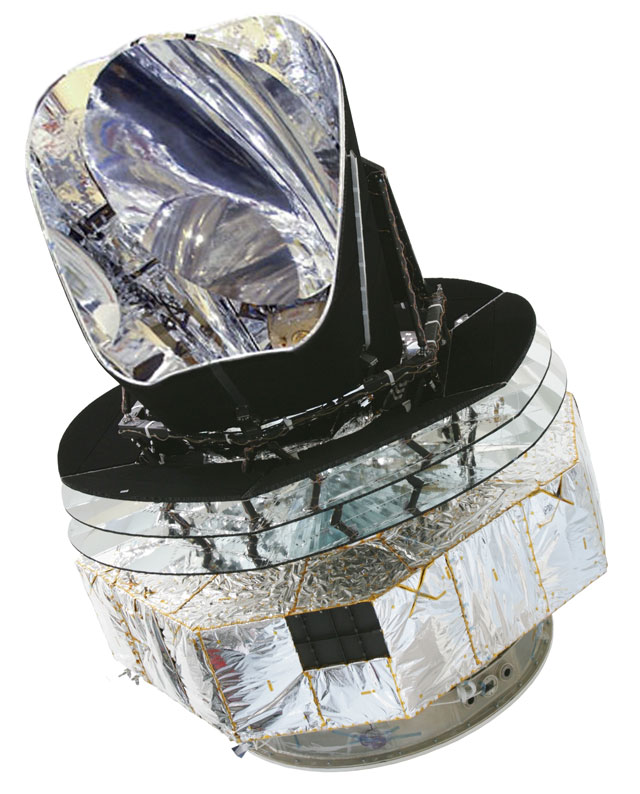
\includegraphics[width=0.5\textwidth]{cosmo_surveys/planck_s.jpg}
    \caption{The Planck satellite.}
    \label{fig:planck}
\end{figure}
The Planck spacecraft was 4.2 metres high and had a maximum diameter of 4.2 metres, with a launch mass of around 1.9 tonnes. The spacecraft comprised a service module, which housed systems for power generation and conditioning, attitude control, data handling and communications, together with the warm parts of the scientific instruments, and a payload module. The payload module consisted of the telescope, the optical bench, with the parts of the instruments that needed to be cooled - the sensitive detector units - and the cooling systems.

Since the end of mission in October 2013, the Planck Collaboration has subsequently released all their data which now constitute the Planck Legacy Archive (PLA) containing all public products originating from the Planck mission. On 17 July 2018 ESA and the Planck Collaboration have released to the public a new and improved version of the data acquired by the Planck satellite, which constitutes the final official release from Planck.

The data from Planck have allowed cosmologists to set very tight constraints on many parameters of the standard model, including the Hubble constant, the densities of baryonic matter, dark matter and dark energy, and the spectral index (for Planck results, see \cite{planck_cosm}).
\section{W-FIRST}
The Wide-Field Infrared Survey Telescope (WFIRST) is a NASA large space mission designed to settle essential questions in dark energy, exoplanets, and infrared astrophysics. It is designed to perform wide-field imaging and slitless spectroscopic surveys of the near infrared sky. The current Astrophysics Focused Telescope Assets (AFTA) design of the mission makes use of an existing 2.4-m telescope to enhance sensitivity and imaging performance. It is the top--ranked large space mission in the New Worlds, New Horizon (NWNH) Decadal Survey of Astronomy and Astrophysics. The main instrument is a wide-field multi-filter NIR imager and spectrometer. With the 2.4-m telescope, a coronagraph instrument has been added to the payload for direct imaging of exoplanets and debris disks. WFIRST was approved for development and launch in 2016 and the mission should start in the mid 2020s \cite{WFIRST_report}.

\begin{figure}[ht]
    \centering
    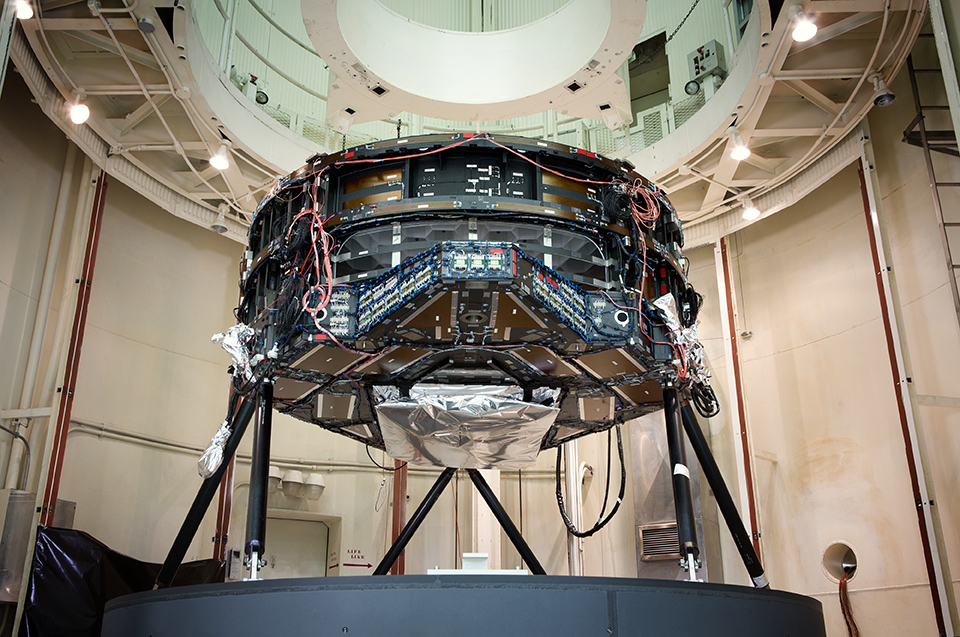
\includegraphics[width=0.9\textwidth]{cosmo_surveys/WFIRST.jpg}
    \caption{Primary Mirror Assembly.}
    \label{fig:wfirst}
\end{figure}
The mission will feature strategic key science programs plus a large program of guest observations. The main focus is on the dark energy and fundamental cosmology (determine the expansion history of the Universe and the growth history of its largest structures). The next scientific goal is discovering of exoplanets -- by microlensing photometric survey of the Galactic bulge and by a direct high-contrast imaging and spectroscopic survey of the nearest stars. Data for general astrophysics science will be gathered by surveys at high Galactic latitudes and Galactic bulge. Relatively huge priority is assigned to the guest observer science program.

The payload features a 2.4-m telescope, which feeds the wide-field instrument (wide-field channel and an integral field unit spectrograph channel) and the coronagraph instrument. The wide-field channel covers a wavelength range 0.76--2.0 \um and a spectroscopy mode covering 1.35--1.89 \um. The wide-field focal plane uses 18 4k $\times$ 4k HgCdTe detector arrays. The integral field unit channel uses an image slicer and spectrograph to provide individual spectra of each slice covering the 0.6--2.0 \um spectral range. The coronagraph instrument provides high-contrast imaging and spectroscopy. Direct imaging is provided over a band--pass of 430--970 nm, while spectroscopy is provided by the spectrograph over the spectral range of 0.6--0.97 \um with a spectral resolution of $R\sim70$ \cite{WFIRST_report}.

As WFIRST will be a NIR mission it will require visible band photometry for photo-z determination. LSST will be the premier ground-based facility to provide those data. As for Euclid, the baryon acoustic oscillation spectroscopic survey will be helpful for calibrating photo-z determinations for LSST. The comparison of shear determinations between WFIRST and LSST measurements will be useful for understanding shape measurement systematics with both facilities.
\chapter{Outlook}
\label{chpt:outlook}
In the thesis we explored ways to study modified gravities. The work was focused on quasi-linear regimes as the full non-linear behavior of modified gravities is hard to study due to its numerical difficulties. In \autoref{chpt:de_mg} we studied the properties of the chameleon gravity in spherical systems -- stars and in NFW halos both on scales of galaxies and clusters of galaxies. Although the results showed that the Hu-Sawicki \fR\ theory is screened in this system, other modifications of gravity do not have to be. Our code and implemented techniques can be used with slight modifications for studies of broader class of theories.

Implementing other models of \fR\ gravity or chameleon gravity should be fairly straightforward and therefore we would like to explore this type of modification in a similar way as we did for the Hu-Sawicki model. We would like to study the the generic \fR\ models with negative and positive powers of curvature of \textcite{2003PhRvD..68l3512N} which can in principle unified the inflation and cosmic acceleration. The models is given by
\eq{
    f(R)=R-\frac{a}{(R-\Lambda_1)^n}+b(R-\Lambda_2)^m\,.
}
Another class of models we would like to explore was proposed in \textcite{2007JETPL..86..157S}. This class of modifications is given by
\eq{
    f(R)=R+\lambda R_0\left[\left(1+\frac{R^2}{R_0^2}\right)^{-n}-1\right]\,.
}
All of these models can be studied in dense objects surrounded by vacuum (or decreasing density) as we did in this work. Another approach we can be tested in laboratory conditions on Earth is opposite -- behavior of the chameleon in vacuum chamber surrounded by dense environment. This could be implemented easily in our code and is therefore worth to study. However, we showed that the effective screening potential is very low on scales of galaxies and therefore we do not expect this will lead to measurable results.

The main field for studying modified gravities remain on cosmological scales where it mimics the cosmological constant. In the work we dealt we approximations which can greatly help to study quasi-linear regimes. Although the non-linear results for used approximation schemes do not look very promising compared to simple particle-mesh codes such as \code{COLA} they proved that linear approximation can be used successfully and we can still obtain results in mildly non-linear regimes. This can be used for studies of modified gravity where solving the full non-linear equations is computationally very demanding and probing the huge space of different modifications almost impossible. We showed that linear approximation of chameleon equations can still lead to observable non-linear results.

This approach we want to pursue further, i.e. to use particle-mesh codes such as \code{COLA}. \code{HACC} or \code{GADGET} without demanding short-range interactions and implement modified equations for theories such as chameleon. To speed up the execution time we would use the linear predictions for these theories which we saw can still lead to non-linear results.

The next step we can make in studying the non-linear regime with modified gravities is to use \nbody\ code with short-range forces, use the linear predictions for chameleon gravity to avoid the lengthy computation of the chameleon field and therefore obtain a good approximation of the background value of the field. To solve the equations on small scales quickly we would use the introduced technique for spherical systems. As the halo finders are a standard part of the simulations, obtaining some approximate density profile of forming halos would not be too expensive. Consequent solving of the one-dimensional chameleon non-linear equations does not pose any substantial demands on computing time.
\chapter*{Conclusion}
\addcontentsline{toc}{chapter}{Conclusion}
% Do autoref \url{http://home.ef.jcu.cz/~houda/publications/2009-dissertation-abstract.pdf}
The thesis was dealing with the topic of modified gravity and how we can discover its resulting deviations from general relativity. In \autoref{chpt:cosmo_evol} we summarized linear equations for the evolution of the Universe. We described how we can use the evolution process to studies of cosmological parameters of the Universe. We described basic cosmological observables and their usefulness when distinguishing between different cosmologies.

\hyperref[chpt:de_mg]{Chapter 2} was focused on modifications of the general relativity. We described successes and failures of the standard cosmological model and presented main issues with the cosmological constant. We described how we can modify the theory of gravity and focused on one of the most studied extensions -- the \fR\ gravity. We studied the Hu-Sawicki \fR\ theory from a different angle of view than most authors -- as the chameleon gravity in the Einstein frame. We studied the chameleon behavior numerically and we checked the linear predictions with our numerical solutions. We studied the chameleon behavior in spherical systems (stars, galaxies, clusters) and concluded that the chameleon mechanism hides the fifth force on scales smaller than superclusters for the Hu-Sawicki model and that the chameleon needs to be studied on large cosmological scales through \nbodysim s. Our original method of solving modified gravity in spherical systems represents an important contribution because it can be applied to other models than Hu-Sawicki \fR. With these methods we can check the behavior of other theories in spherical systems and also check their behavior in laboratory conditions on the Earth.

In \autoref{chpt:cosmo_sim} we described general techniques when dealing with cosmological \nbodysim s and how we implemented them in our own code for \nbodysim s -- with both standard and modified gravity. We described our own contribution to the \code{CCL} code and how the \code{CCL} can help scientists worldwide to speed up their work on cosmology.

In \autoref{chpt:app_schemes} we introduced different approximations that can be used to study the Universe quickly and intuitively. Most of the previous studies focused on the Einstein--de Sitter Universe whereas in this work we generalized the equations to the \LCDM\ cosmology. We described how we implemented these approximations in studies of modified gravity which has not been done before and is one of the original result of this work.

Key results of the thesis are presented in \autoref{chpt:app_sims}. We described original results of our cosmological \nbodysim s using approximate schemes. We focused on aspects that have drawn less attention in the past -- slower growth of structure formation (modified growth function), study of the correlation function, predictions of the shape of the peak of baryonic acoustic oscillations in real space and the ability to predict certain non-linear features of full \nbodysim s. We showed that these approximations can be used to study scales around the baryon acoustic oscillation scale, $k\sim 0.1~h\text{Mpc}^{-1}$ but not much further. We also tested these methods on the chameleon gravity and showed what probes are suited the best for distinguishing between different parameters of the chameleon gravity. Unlike matter power spectra and baryonic acoustic oscillation, the halo mass function does not seem to be a good way to study the chameleon gravity. In \autoref{chpt:outlook} we then discussed other possible applications of approximate methods described in this work and we outlined further course of our studies.

In \autoref{chpt:cosmo_surveys} we reviewed the present-day and future experiments designed to study our Universe. We showed what constraints on our Universe have already been observed and what accuracy of future experiments we can expect.

\subsubsection{Author's publications}
\begin{refsection}[bibliography/my_work.bib]
In the \hyperref[chpt:list_publish]{List of publications} all author's publications are listed (in alphabetical order by the authors' last names). The list includes the author's previous work in the Cherenkov Telescope Array collaboration \parencite{2016arXiv161005151C,2017arXiv170903483A,2017ApJ...840...74A,2019scta.book.....C}. While working on the CTA, the author's main interest were the atmospheric simulations of cosmic showers \parencite{2017EPJWC.14401014V,}. The purpose of these simulations is to improve the calibration of the atmospheric properties as well as a calibration of the detector response. One of the main contributions to the systematic uncertainties of the CTA measurements stems from the uncertainty on the atmospheric density profile, of molecules and aerosols, which these simulations help to reduce.

The author's work inside the Dark Energy Science Collaboration (DESC) focused mainly on improving the Core Cosmology Library \parencite[\code{CCL},][]{2019ascl.soft01003C,2019ApJS..242....2C}. Initially, the author helped to create a documentation of the library, wrote many examples of usage of the \code{CCL}, and presented with other authors the \code{CCL} and its capabilities at several sessions to new users. The author also helped to improve several automatization processes regarding the releasing of the library and helped to improve its compatibility across different operating systems and environments.

The author's main work, \textit{Fast approximate methods for modified gravity cosmological simulations} \parencite[published in Monthly Notices of the Royal Astronomical Society,][]{2020MNRAS.493.2085V}, summarizes results regarding the cosmological \nbodysim s described in this work (\autoref{chpt:cosmo_sim} -- \autoref{chpt:app_sims}). It is the result of several-year research regarding the cosmological simulations. During this time, the author wrote his own code for cosmological simulations, implemented methods for solving highly non-linear equations, and developed complex pipelines for processing and analyzing data of these simulations.
\end{refsection}



%%% Bibliography
\cleardoublepage
\phantomsection
\renewcommand{\bibname}{Bibliography}
\addcontentsline{toc}{chapter}{\bibname}
\begingroup
\sloppy
\printbibliography[title={\bibname}]
\endgroup

%%% Figures used in~the~thesis (consider if this is needed)
%\listoffigures

%%% Tables used in~the~thesis (consider if this is needed)
%%% In~mathematical theses, it could be better to~move the~list of~tables to~the~beginning of~the~thesis.
%\listoftables

%%% Doctoral theses must contain a~list of~author's publications
\cleardoublepage
\phantomsection
\renewcommand{\bibname}{List of~publications}
\addcontentsline{toc}{chapter}{\bibname}
\label{chpt:list_publish}
\begin{refsection}[bibliography/my_work.bib]
\nocite{*}
\begingroup
\sloppy
\printbibliography[title={\bibname}]
\endgroup
\end{refsection}

%%% Attachments to~the~doctoral thesis, if any. Each attachment must be
%%% referred to~at~least once from the~text of~the~thesis. Attachments
%%% are numbered.
%%%
%%% The~printed version should preferably contain attachments, which can be
%%% read (additional tables and~charts, supplementary text, examples of
%%% program output, etc.). The~electronic version is more suited for~attachments
%%% which will likely be used in~an~electronic form rather than read (program
%%% source code, data files, interactive charts, etc.). Electronic attachments
%%% should be uploaded to~SIS and~optionally also included in~the~thesis on~a~CD/DVD.
%%% Allowed file formats are specified in~provision of~the~rector no. 72/2017.
%\appendix
%\chapter{Attachments}

%\section{First Attachment}

\openright
\end{document}
